%   D O C U M E N T   P R E A M B L E
% Specify the document class, default style attributes, and page dimensions, etc.
% For hyperlinked PDF, suitable for viewing on a computer, use this:
\documentclass[letterpaper,12pt,titlepage,oneside,final,usenames,dvipsnames]{book}

% \usepackage{XCharter}
% \renewcommand{\rmdefault}{XCharter}
% \usepackage{textcomp} % Add the textcomp package

 
% For PDF, suitable for double-sided printing, change the PrintVersion variable below to "true" and use this \documentclass line instead of the one above:
%\documentclass[letterpaper,12pt,titlepage,openright,twoside,final]{book}

% Some LaTeX commands I define for the document nomenclature.
\newcommand{\die}[2]{\frac{\partial #1}{\partial #2}}
\newcommand{\package}[1]{\textbf{#1}} % package names in bold text
\newcommand{\cmmd}[1]{\textbackslash\texttt{#1}} % command name in tt font 
\newcommand{\href}[1]{#1} % does nothing, but defines the command so the print-optimized version will ignore \href tags (redefined by hyperref pkg).
%\newcommand{\texorpdfstring}[2]{#1} % does nothing, but defines the command
% Anything defined here may be redefined by packages added below...
% This package allows if-then-else control structures.
\usepackage{ifthen}
\newboolean{PrintVersion}
\setboolean{PrintVersion}{false}
% CHANGE THIS VALUE TO "true" as necessary, to improve printed results for hard copies by overriding some options of the hyperref package, called below.

%\usepackage{nomencl} % For a nomenclature (optional; available from ctan.org)
\usepackage{amsmath,amssymb,amstext} % Lots of math symbols and environments
\usepackage[pdftex]{graphicx} % For including graphics N.B. pdftex graphics driver 

%----------------------------------------------------------------------
%   A D D  H E R E
% Packages added for Kirsten's dissertation
% \usepackage{geometry}
\usepackage{changepage}
\usepackage{epigraph}
\setlength\epigraphwidth{.8\textwidth}
\usepackage[absolute]{textpos}
% \usepackage{setspace}
% \usepackage{xcolor, tikz}
% \usetikzlibrary{chains,fit}
% \usepackage{tikz}
% \usetikzlibrary{shadings, shadows, shapes, arrows, calc, positioning, shapes.geometric, arrows.meta, patterns, patterns.meta}
\usepackage{xcolor, tikz}
\usetikzlibrary{chains,fit, shadings, shadows, shapes, shapes.geometric, arrows, calc, positioning, shapes.geometric, arrows.meta, patterns, patterns.meta}

\tikzstyle{startstop} = [rectangle, rounded corners, minimum width=3cm, minimum height=1cm,text centered, draw=black, fill=red!30]
\tikzstyle{process} = [rectangle, minimum width=3cm, minimum height=1cm, text centered, draw=black, fill=orange!30]
\tikzstyle{decision} = [rectangle, minimum width=3cm, minimum height=1cm, text centered, draw=black, fill=green!30]
\tikzstyle{arrow} = [thick,->,>=stealth]

\usepackage{listings}

\definecolor{codegreen}{rgb}{0,0.6,0}
\definecolor{codegray}{rgb}{0.5,0.5,0.5}
\definecolor{codepurple}{rgb}{0.58,0,0.82}
\definecolor{backcolour}{rgb}{0.95,0.95,0.92}

% Code style examples 
% https://github.com/srinadhu/RL_Pacman/blob/master/report.pdf
% https://www.overleaf.com/learn/latex/Code_listing

\lstdefinestyle{mystyle}{
    language=Python,
    backgroundcolor=\color{backcolour},   
    commentstyle=\color{codegreen},
    keywordstyle=\color{magenta},
    numberstyle=\tiny\color{codegray},
    stringstyle=\color{codepurple},
    basicstyle=\ttfamily\footnotesize,
    breakatwhitespace=false,         
    breaklines=true,                 
    captionpos=b,                    
    keepspaces=true,                 
    numbers=left,                    
    numbersep=5pt,                  
    showspaces=false,                
    showstringspaces=false,
    showtabs=false,                  
    tabsize=2
}

\lstset{style=mystyle}

% \definecolor{dkgreen}{rgb}{0,0.6,0}
% \definecolor{gray}{rgb}{0.5,0.5,0.5}
% \definecolor{mauve}{rgb}{0.58,0,0.82}
% \lstset{frame=tb,
%   language=Java,
%   aboveskip=3mm,
%   belowskip=3mm,
%   showstringspaces=false,
%   columns=flexible,
%   basicstyle={\small\ttfamily},
%   numbers=none,
%   numberstyle=\tiny\color{gray},
%   keywordstyle=\color{blue},
%   commentstyle=\color{dkgreen},
%   stringstyle=\color{mauve},
%   breaklines=true,
%   breakatwhitespace=true,
%   tabsize=3
% }

% \newcommand\pythonstyle{\lstset{
% language=Python,
% basicstyle=\ttm,
% morekeywords={self},              % Add keywords here
% keywordstyle=\ttb\color{deepblue},
% emph={MyClass,__init__},          % Custom highlighting
% emphstyle=\ttb\color{deepred},    % Custom highlighting style
% stringstyle=\color{deepgreen},
% frame=tb,                         % Any extra options here
% showstringspaces=false
% }}

% \usepackage{epstopdf}
\usepackage{catchfilebetweentags}
\usepackage{rotating} %DRR Sidewayas
\DeclareGraphicsRule{.tif}{png}{.png}{`convert #1 `dirname #1`/`basename #1 .tif`.png}
\usepackage{pgfplots}
% Add this line to set the compatibility mode
\pgfplotsset{compat=1.17}
%\usepackage[dvipsnames]{xcolor}
%\setpalette("R4")
%----------------------------------------------------------------------

% Hyperlinks make it very easy to navigate an electronic document.
% In addition, this is where you should specify the thesis title and author as they appear in the properties of the PDF document.
% Use the "hyperref" package 
% N.B. HYPERREF MUST BE THE LAST PACKAGE LOADED; ADD ADDITIONAL PKGS ABOVE
\usepackage[pdftex,pagebackref=false]{hyperref} % with basic options
%\usepackage[pdftex,pagebackref=true]{hyperref}
		% N.B. pagebackref=true provides links back from the References to the body text. This can cause trouble for printing.
\hypersetup{
    plainpages=false,       % needed if Roman numbers in frontpages
    unicode=false,          % non-Latin characters in Acrobat’s bookmarks
    pdftoolbar=true,        % show Acrobat’s toolbar?
    pdfmenubar=true,        % show Acrobat’s menu?
    pdffitwindow=false,     % window fit to page when opened
    pdfstartview={FitH},    % fits the width of the page to the window
%    pdftitle={uWaterloo\ LaTeX\ Thesis\ Template},    % title: CHANGE THIS TEXT!
%    pdfauthor={Author},    % author: CHANGE THIS TEXT! and uncomment this line
%    pdfsubject={Subject},  % subject: CHANGE THIS TEXT! and uncomment this line
%    pdfkeywords={keyword1} {key2} {key3}, % list of keywords, and uncomment this line if desired
    pdfnewwindow=true,      % links in new window
    colorlinks=true,        % false: boxed links; true: colored links
    linkcolor=blue,         % color of internal links
    citecolor=green,        % color of links to bibliography
    filecolor=magenta,      % color of file links
    urlcolor=cyan           % color of external links
}
\ifthenelse{\boolean{PrintVersion}}{   % for improved print quality, change some hyperref options
\hypersetup{	% override some previously defined hyperref options
%    colorlinks,%
    citecolor=black,%
    filecolor=black,%
    linkcolor=black,%
    urlcolor=black}
}{} % end of ifthenelse (no else)

\usepackage[automake,toc,abbreviations]{glossaries-extra} % Exception to the rule of hyperref being the last add-on package
% If glossaries-extra is not in your LaTeX distribution, get it from CTAN (http://ctan.org/pkg/glossaries-extra), 
% although it's supposed to be in both the TeX Live and MikTeX distributions. There are also documentation and 
% installation instructions there.

% Setting up the page margins...
% uWaterloo thesis requirements specify a minimum of 1 inch (72pt) margin at the
% top, bottom, and outside page edges and a 1.125 in. (81pt) gutter margin (on binding side). 
% While this is not an issue for electronic viewing, a PDF may be printed, and so we have the same page layout for both printed and electronic versions, we leave the gutter margin in.
% Set margins to minimum permitted by uWaterloo thesis regulations:
\setlength{\marginparwidth}{0pt} % width of margin notes
% N.B. If margin notes are used, you must adjust \textwidth, \marginparwidth
% and \marginparsep so that the space left between the margin notes and page
% edge is less than 15 mm (0.6 in.)
\setlength{\marginparsep}{0pt} % width of space between body text and margin notes
\setlength{\evensidemargin}{0.125in} % Adds 1/8 in. to binding side of all 
% even-numbered pages when the "twoside" printing option is selected
\setlength{\oddsidemargin}{0.125in} % Adds 1/8 in. to the left of all pages when "oneside" printing is selected, and to the left of all odd-numbered pages when "twoside" printing is selected
\setlength{\textwidth}{6.375in} % assuming US letter paper (8.5 in. x 11 in.) and side margins as above
\raggedbottom

% The following statement specifies the amount of space between paragraphs. Other reasonable specifications are \bigskipamount and \smallskipamount.
\setlength{\parskip}{\medskipamount}

% The following statement controls the line spacing.  
% The default spacing corresponds to good typographic conventions and only slight changes (e.g., perhaps "1.2"), if any, should be made.
\renewcommand{\baselinestretch}{1} % this is the default line space setting

% By default, each chapter will start on a recto (right-hand side) page.
% We also force each section of the front pages to start on a recto page by inserting \cleardoublepage commands.
% In many cases, this will require that the verso (left-hand) page be blank, and while it should be counted, a page number should not be printed.
% The following statements ensure a page number is not printed on an otherwise blank verso page.
\let\origdoublepage\cleardoublepage
\newcommand{\clearemptydoublepage}{%
  \clearpage{\pagestyle{empty}\origdoublepage}}
\let\cleardoublepage\clearemptydoublepage

% Define Glossary terms (This is properly done here, in the preamble and could also be \input{} from a separate file...)
% Main glossary entries -- definitions of relevant terminology

% \newglossaryentry{}
% {
% name=,
% description={}
% }

% \newglossaryentry{}
% {
% name=,
% description={}
% }

\newglossaryentry{agglomeration economies}
{
name=agglomeration economies,
description={economic efficiencies resulting from \gls{agglomeration effects}.}
}

\newglossaryentry{agglomeration}
{
name=agglomeration,
description={A collection of similar items in one location. A city is an agglomeration of people and generally of firms. Agglomeration may have properties that individuals do not have, giving rise to \gls{agglomeration effects} or gls{agglomeration economies} }
}

\newglossaryentry{migration equilbrium}
{
name= migration equilbrium,
description={A situation in which not resident will hke herself better off by migrating to or between cities or countries. Similar to a migration equilibrium.}
}


\newglossaryentry{locational equilibrium}
{
name=locational equilibrium,
description={A situation in which no resident will hke herself better off by moving to another location. A Nash equilibium with housing efficiently allocated  given market prices. See \gls{migration equilbrium}.}
}


\newglossaryentry{agglomeration effects}
{
name=agglomeration effects,
description={An effect of increasing number of firms  or workers in one place. A larger, deeper, more specialized labor pool enables workers to better match their skills to the needs of firms or creates knowledge spillovers in which firms and workers learn from each other.}
}

\newglossaryentry{monopolistic competition}
{
name=monopolistic competition,
description={A type of imperfect competiton. Perfect competition is a description of a market with many seller, all of whom are price takers. Monopoly is a market with a single seller, who therefore has the power to set the selling price. Monopolistic competition describes cases in between, with sellers that have some power to set prices within a segment of the market. It occurs when many companies offer competing products or services that are similar, but are not perfect, substitutes.}
}

\newglossaryentry{labour adjustment cost}
{
name=labour adjustment cost,
description={Costs associates with hiring , firing or training that prevent or slow the rate as which a firm will increase of decrease the number of workers it employs.}
}

\newglossaryentry{frictional unemployment}
{
name=frictional unemployment,
description={the part of total unemployment  due to people being in the process of voluntairily moving from one job to another.}
}

\newglossaryentry{marginal product}
{
name=marginal product,
description={See \gls{marginal product of labour}.}
}

\newglossaryentry{monopoly}
{
name=monopoly,
description={ Market power means you can price above marginal costs. Need free entry to get rid of it. -- it doesn't drive out profit - profits can be sustained over longer. Monopolist can charge a higher price but pays competitive price for all inputs including labour. If a firm also had a monopoly on offering jobs, they could drive down wages.}
}

\newglossaryentry{duopoly}
{
name=duopoly,
description={A market with two sellers. Under one set of assumptions the result will  be the monopoly price, under others,  the situation will generate lower  than monopoly prices, ore even competitive pricing and may result in market instability}
}

\newglossaryentry{monopsony}
{
name=monopsony,
description={A market with one buyer that therefore has market power.}
}

\newglossaryentry{imperfect information}
{
name=imperfect information,
description={ the buyers and/or sellers do not have all the information necessary to make an informed decision. }
}

\newglossaryentry{externalities}
{
name=externalities,
description={any indirect costs or benefit to uninvolved third parties that are an effect of a decision-makers activity but are not included in the decision-maker's cost-benefit calculations. Lawn mowers may wake the neighour, emissions form vehicles cause emphysema, burning fossil fuels may contribute to climate change, or painting your house may raise the value of the neighbour's house. In our model, when employer increase their workforce there is a positive effect on the productivity of all other workers in the city. This is an external effect}
}

\newglossaryentry{constant returns to scale}
{
name=constant returns to scale \gls{CRS}. ..,
description={when doubling all inputs results in exactly double the output. }
}

\newglossaryentry{competitive market}
{
name=competitive market,
description={**FIX Everybody is a price taker. Price takers don't assume anything they do affects other producers or suppliers, so they act in terms of their internal prices and costs.
This means their decision making process doesn't take into account any one else's behaviour.
? The easy way to see that is assume prices are fixed - all that's required to get the behaviour. ..  have a few other things like free exit and entry, perfect information etc -- to get the efficiency result. - (or to ensure price taking)}
}

\newglossaryentry{effective labour}
{
name=effective labour,
description={FIX - Effective labour is the productive output from labour. As soon as you introduce agglomeration economies, labour becomes a more complex phenomena. There is the benefit of the single worker which should be perfectly declining on that nice concave production function and there is the diagonal movement as a result of increasing productivity because you keep adding people to the market. That means that your productivity of the worker isn't' just attached to the worker and your plant. It has this other component.. 'effective labour' -- the output including the A term.}
}

\newglossaryentry{spillover effects}
{
name=spillover effects,
description={ \Gls{externalities} are the most commonly discussed form of spillover effects but any economic event in one context that occurs because of something else in a seemingly unrelated context can be considered a spillover. It is a looser term than externality because an externality is a consequence, at least in economic theory, of rational optimizing behaviour.}
}

\newglossaryentry{substitutable}
{
name=substitutable,
description={One good may be substituted for another without loss of benefit. Two brands of motor or are good substitutes for each other. Oranges are somewhat subsitutable for apples , but not for screwdrivers.}
}

\newglossaryentry{neoclassical distribution theory}
{
name=neoclassical distribution theory,
description={A theory that states that in perfect competition the owner of every unit of every  factor of production will be paid precisely the  value of the \gls{marginal product} of that factor for each unit unit they contribute to production. }
}

\newglossaryentry{Solow-Swan model}
{
name=Solo-Swan model,
description={}
}

\newglossaryentry{marginal product of labour}
{
name=marginal product of labour,
description={Firms calculate what the next worker is worth to them. That's what they're willing to pay for labour. 
This is the labour demand function based on the \gls{marginal product} which is declining. When a firm has only a few workers, it is high on that demand function, and has to move down. It cuts workers. If it's too low, it expands and hires. %This says something about the geometry of what employers could pay. 
% Firms can't pay workers more than they can earn in the long term, unless that money comes from somewhere, but they could push down wages and extract more profit, invest more in other factors of production, etc.
}
}

\newglossaryentry{migration equilibrium}
{
name=migration equilibrium,
description={The theoretical situation in which no resident can  make themselves better off by moving to another location. It is a logical consequence of utility maximization and free mobility that results in a Pareto optimal allocation of housing. Technically it is a Nash equilibrium, While extremely useful in analysing urban systems, the concept does not closely describe real cities.  }
}

\newglossaryentry{commuter shed}
{
name=commuter shed,
description={for a city, the area over which people will travel to work in a city. In the Alonzo-Jacobs model, it is sharply defined by the maximum distance commuters can travel before transportation costs exceed the wage premium. In  practice, the duration of commutes is highly variable. It is greater in the case of men, singles, educated and foreign workers, persons living in rented housing, using public transport, living or working in large cities, or working in large firms,  and when the  unemployment rate is high.\cite{axisaFactorsInfluencingCommute2012} }
}

\newglossaryentry{circular city}
{
name=circular city,
description={In urban theory, an idealized city form predicted by models with uniform travel costs in all directions and a fixed household commuting budget. If a city is laid out on a rectangular grid, the same travel-cost logic yields a rectangular city. Recently the term is applied to cities committed to achieving a circular economy. }
}

\newglossaryentry{radial city}
{
name=radial city,
description={A radial concentric city plan is formed by streets that extend outward from a defined center and reach the outer edge of the city, together with concentrically arranged roads that connect the radial streets to the lots. it is an idealized pattern that traces back to ancient times and appears  today in planned cities and districts. See \gls{circular city}.}
}

\newglossaryentry{surplus}
{
name=surlpus,
description={Or economic surplus. Any social product in excess of the minimum required to reproduce society. In value terms the surplus appears as profit or rent and accrues to the owner of a  scarce input that varys in quality, such as land. In the mid-19th century, French engineer Jules Dupuit first extended the concept of economic surplus to what came to be called producer- and consumer-surplus.}
}

\newglossaryentry{Alonzo-Jacobs model}
{
name=Alonzo-Jacobs model,
description={A model combining the Alonzo model  associated with  William Alonso \cite{alonsoModelUrbanLand1960} with the \gls{agglomeration} theory of Jane Jacobs \cite{jacobsEconomyCities1969a}. }
}

\newglossaryentry{monopsonist}
{
name=monopsonist,
description={..}
}

\newglossaryentry{financial return}
{
name=financial return,
description={MAYBE ADD what is best definition? - there may be other returns. Assessed by comparing the net rent $\mathcal{R}_N$ to the costs of acquiring a property, in particular to the cost of borrowing money. CLARIFY}
}

\newglossaryentry{home services}
{
name=home services,
description={A property offers two kinds of services: home services and \gls{locational services}. Home services describes the value offered by living in a house: a place to sleep, to prepare food, the amenity of being in the home, etc. Since people require housing inside and outside the city, home services are modeled as paid for as a share of the subsistence wage ($a \psi$).}
}

\newglossaryentry{locational services}
{
name=locational services,
description={A property offers two kinds of services: \gls{home services} and locational services. Locational services are services accessed by right of location. They include access to the central city job, access to locational amenity, and the benefit of services and connections associated with a location. In the core model, Locational services are, on an annual basis, the rent premium $w$, minus the transportation costs $c$ for a property a given distance, $d$, from the center, $\omega- {dc}$.}
}

\newglossaryentry{rent share}
{
name=rent share,
description={..}
}

\newglossaryentry{Pareto efficiency}
{
name=Pareto efficiency,
description={An economic state where resources cannot be reallocated to make one individual better off without making at least one individual worse off.}
}

\newglossaryentry{efficiency conditions}
{
name=efficiency conditions,
description={Conditions derived in neoclassical economic theory that must be satisfied if a system or activity is to achieve Pareto efficiency. Under somewhat reasonable conditions the efficiency conditions are achieved by agents acting in a decentralized manner to maximize their own profit or utility.}
}

\newglossaryentry{neoclassical economics}
{
name=neoclassical economics,
description={An approach to the study of the economy and economic behaviour that attempts to explain the production, pricing, consumption of goods and services,  through supply and demand, and to explain agent behaviour using a theory of rational agents who satisfy \gls{marginal} efficiency conditions. It integrates, within a mathematical framework, the cost-of-production theory  developed from \gls{classical economics} with a consumer demand theory based on utility maximization.}
}

\newglossaryentry{classical economics}
{
name=classical economics,
description={Or classical political economy. A school of thought in political economy that flourished, primarily in Britain, in the late 18th and early-to-mid 19th century. Its main thinkers include Adam Smith, Jean-Baptiste Say, David Ricardo, Thomas Robert Malthus, and John Stuart Mill. After 1870s the key features of the classical approach weer carried forward by  Karl Marx and his followers and  Henry George.}
}

\newglossaryentry{socioeconomic status}
{
name=socioeconomic status,
description={Socioeconomic status is typically broken into three levels, high, middle, and low,  commonly referred to as ``upper class'', ``middle class'', and ``working or lower class'', it differs from `\gls{class}' in the more traditional sense, which is a functional classification. See \gls{Ricardian class}, being based on occupation, income, family wealth.}
}

\newglossaryentry{Ricardian class}
{
name=Ricardian class,
description={The conception of class in \gls{classical economics} including Marx, where class is based on the types and amounts of productive capital the individual owns. See \gls{class}.}
}

\newglossaryentry{rent profile}
{
name=rent profile,
description={see \gls{bid-rent function} or \gls{bid-rent curve}}
}

\newglossaryentry{class}
{
name=class,
description={This term has a wide range of sometimes conflicting meanings. In our usage, which is consistent with classical economics including Marx class is based on the types and amounts of productive capital the individual owns. This is a functional definition quite distinct from socioeconomic status which is more common in the current discussion. Our treatment of the evolution of class structure with financialization draws on We allow  people in different functional classes to own financial capital, producing intermediate classes \`a la Roemer\cite{roemerGeneralTheoryExploitation1982}.}
}
\newglossaryentry{capitalize}
{
name=capitalize,
description={To capitalize a stream of expected income is to compute it's capitalized value. Capitalized value is the current worth of an asset, usually real estate, based on a calculation of present value of expected income over the course of its economic lifespan.}
}

\newglossaryentry{agglomeration effect}
{
name=agglomeration effect,
description={The external economies associated with size and concentration. The benefits of size and concentration vary for different cross-sections of the urban population. Three such groupings may be identified: 1. Consumer agglomeration economies; Business agglomeration economies; Social agglomeration economies \cite{carlinoAgglomerationEconomiesSurvey1978}.}
}

\newglossaryentry{price bubble}
{
name=price bubble,
description={The sustained rise in the price of an asset above its ``normal'' market value'' caused by agents (mainly speculators) forecasting further price increases base on previous increases, rather than on estimates on intrinsic value.  Price bubbles are sustained by expectations of future increases in the price of an asset. They may end sharply, or crash, when expectations shift.}
}

\newglossaryentry{marginal value-product}
{
name=marginal value-product,
description={Also known as the marginal revenue product. The marginal revenue created due to an addition of one unit of productive resource, such as one more worker. Calculated by multiplying the marginal physical product by the price, or the marginal revenue in the case of a non-competitive market.}
}

\newglossaryentry{neoclassical growth theory}
{
name=neoclassical growth theory,
description={An economic theory that outlines how a steady economic growth rate results from a combination of three driving forces—labor, capital, and technology. Robert Solow and Trevor Swan developed and introduced the model of long-run economic growth in 1956. It is the  foundation of most empirical and theorical attempts to explain macroeconomic growth.}
}

\newglossaryentry{financial capital}
{
name=financial capital,
description={The word "capital" has many different meanings in economics and finance. Financial capital is simply lendable purchasing power. Owners of financial capital provide their liquidity to borrowers in exchange for a future return. Interest rates are the prices charged for the use of financial capital. It is generally based on (secured by) ownership of tradable assets.  Anything can be a form of financial capital as long as it has a monetary value and can be  used in the pursuit of future revenue. Marx distinguished  financial capital (then called circulating capital or money capital) from fixed or real capital.}
}

\newglossaryentry{agent-based model}
{
name=agent-based model,
description={Agent-based models are computer simulations used to study the interactions between people, things, places, and time. They are usually stochastic models built from the `bottom up,' meaning by modelling individual agents (people, institutions, etc). Agents essentially sub-programs that respond to other agents and the environment in certain ways. These interactions produce emergent effects that may differ from the results of traditional, regression-based methods in that, like systems dynamics modeling, it allows for the exploration of complex systems that display non-independence of individuals and feedback loops in causal mechanisms.}
}

\newglossaryentry{urban scaling}
{
name=urban scaling,
description={Urban scaling laws reliably relate socio-economic, behavioural and physical variables to the population size of cities. They allow for approaches  to city planning and for an understanding of urban resilience and economics. In this thesis we use the well-established relationship between population and urban productivity. \cite{doi:10.1098/rsif.2020.0705}}. %\gls{}.}
}


\newglossaryentry{classical rent theory}
{
name=classical rent theory,
description={explained how land generated surplus value for its owner and how this surplus explained the wealth and income of the land-owning class. David Ricardo produced the classic description in 1815 based on extensive prior analysis by others in the preceding century. The key notion is the ``marginal'' unit of land. It is just barely worth putting this land into production because it just barely produces enough to justify the cost of production, and transportation. More productive land or better located land produces a surplus that the landowner  collects in the form of land rent collected from tenant farmers. No tenant would pay to cultivate the  marginal unit of land. The theory employed the basic logic of later the later ``marginalist''  school of economic analysis. = See \gls{class}, \gls{rent}.}
}

\newglossaryentry{rent}
{
name=rent,
description={The economic  surplus generated in production as a result of differences in the quality of some factor of production. Often described as the difference between the opportunity cost of a factor of production and the income it earns. In this theses we focus on rents generated by \glspl{agglomeration effect}. According to \gls{classical rent theory}, rent is the price paid for the use of land. More generally it is the  surplus generated by any natural resource, up to and including the athletic talents of basketball stars.\cite{lackmanClassicalBaseModern1976} Land, talent and mineral resources are seen as ``the free gift of nature'', forms of capital which the owners do not create but do appropriate. Like the productivity of agricultural land in classical theory,  urban \gls{agglomeration effect}s produce land rents that are not created but are appropriated by the landowners. See \gls{class}.}
}

\newglossaryentry{maximum bid function}
{
name=maximum bid function,
description={A function that generates the maximum that an investor would bid for a property.  See \gls{bid-rent curve}, \gls{bid-rent function}.}
}

\newglossaryentry{bid-rent function}
{
name=bid-rent function ,
description={See \gls{bid-rent curve}.}
}

\newglossaryentry{reservation price}
{
name=reservation price,
description={Seller's minimum price of to accept a bid. If no offer is at least as large as the reservation price, the seller is effectively the buyer. It is lowest price that a prospective seller will accept, and is computed as seller's maximum bid price, which incorporates the net rent achievable.}
}

\newglossaryentry{bid-rent curve}
{
name=bid-rent curve,
description={The height of a graph showing distance from employment horizontally and the amount that residents will pay to rent land at that distance. It is also also called a \gls{rent profile}. With varying agents and property attributes can be seen a set of functions of location, each of which  generates a bid price for one category of agent.   See \gls{rent premium}, .}
}

\newglossaryentry{borrowing ratio}
{
name=borrowing ratio,
description={$m$. The maximum fraction of the price of a property that may be mortgaged. Determined by the bank (the lender) based on individual wealth and income. }
}

\newglossaryentry{rent premium}
{
name=rent premium,
description={or \gls{warranted economic rent} is the excess rent  that might be charge for the use of urban land relative the non-urban land. In our model the rent premium for an urban property is equal to the urban wage premium minus the transportation costs. }
}

\newglossaryentry{warranted rent}
{
name= warranted rent,
description={$\mathcal{R}_N$ at an  urban location  $d$ units from the centre, is the the value of the flow of services provided by the property, including the locational value, or \gls{warranted economic rent}. It is level of land rent that would be expected in equilibrium based on location and transportation costs.  (It may not be the rent actually charged to a tenant.) }
}

\newglossaryentry{warranted price}
{
name= warranted price,
description={$\mathcal{R}_N$ at an  urban location  $d$ units from the centre, capitalized value of the flow of services provided by the property, the \gls{warranted rent}. 
which  includes locational value, or \gls{warranted economic rent}, (It may differ from the market price) }}

\newglossaryentry{warranted economic rent}
{
name=warranted economic rent,
description={The locational value of an urban property. A surplus generated by \glspl{agglomeration effect}, equal to the urban (wage premium) minus transportation costs, $\omega-{c} d$). This is the the amount that an equilibrium market rent for a property would be expected to exceed the market rent for a similar non-urban property.}
}

\newglossaryentry{net rent}
{
name=net rent,
description={Or net market rent. The warranted rents minus taxes and maintenance costs.}
}

% \newglossaryentry{rent share}
% {
% name=rent share,
% description={..}
% }

% rent paid
% economic rent
% locational rent

\newglossaryentry{marginal}
{
name=marginal,
description={relating to or situated at the edge or margin of something. In the marginalist approach to economics, it  refers to technique of focusing on the cost or benefit of the next unit or individual.}
}

\newglossaryentry{inframarginal}
{
name=inframarginal,
description={Coming before the margin is reached. For example, if the wage is $x$, all workers willing to work for less than $x$ are inframarginal. They are selling their time for more that it is worth to them. They come out ahead on the bargain. Workers who will work for $x$ but not a penny less are marginal. Similarly, with land, the most remote or the least productive land in use is ``marginal'' while  inframarginal land is more productive and generates a \gls{surplus}.}
}

\newglossaryentry{subsistence wage}
{
name=subsistence wage,
description={In our model, the wage which covers the cost of buildings, food and other living costs and a base cost of land. In most urban models this base cost is  the opportunity cost of agricultural land. We have extended the technique to include the opportunity cost of urban labour. }
}

\newglossaryentry{overlapping generations model}
{
name=overlapping generations model,
description={In the \gls{OLG} model individuals live a finite length of time, long enough to overlap with at least one period of another agent's life. The OLG model is the natural framework for the study of life-cycle behavior (investment in human capital, work and saving for retirement).}
}

\newglossaryentry{stylized facts}
{
name=stylized facts,
description={Economists use this term for observations that are widely understood to be empirical truths, to which theories must fit.  Also described as, ``broad tendencies that aim to summarize the data, offering essential truths while ignoring individual details''. The term "stylized facts" was introduced by the economist Nicholas Kaldor in the context of a debate on economic growth theory in 1961 \cite{kaldorCapitalAccumulationEconomic1961}.}
}

\newglossaryentry{perfect foresight}
{
name=perfect foresight,
description={The correct prediction of future events. If agents have  all relevant information and  a correct model to use for prediction. When there is uncertainty it is not possible to have perfect foresight. In solving a complex intertemporal model, economists may assume agents have perfect foresight. This is called the rational expectations approach.}
}

\newglossaryentry{equilibrium reasoning}
{
name=equilibrium reasoning,
description={Gls{equilibrium} analysis identifies variable values of particular interest because they are likely to exhibit stability or capture the implications of the goals of agents. Using these equilibrium values and how they are likely to change in the regions of an equilibrium draw conclusions to is `equilibrium reasoning' because it bases the conclusions on assumptions about the behaviour of the variables near an equilibrium. Equilibrium reasoning implicitly  assumes that the variables will tend to stay near and smoothly approach the equilibrium.}
}

\newglossaryentry{equilibrium}
{
name=equilibrium,
description={In economics and other sciences, an equilibrium is a situation in which forces such as supply and demand are balanced, and in the absence of external influences the (equilibrium) values of variables will not change. In economics an equilibrium is usually understood behaviourally as a situation in which no agent has an incentive to change behaviour given what others are doing. Such a situation is called a Nash Equilibrium or a Cournot-Nash equilibrium.}
}

\newglossaryentry{expectations}
{
name=expectations,
description={Predictions of future events or values, formed by agents for use in decision-making. Agents may form their expectations by looking backward at data on previous values, or by projecting forward using a mental model of how the system works. If agents are fully informed about the state of the system and how it works, their expectations are essentially the same as the predictions of the relevant economic theory and they are termed `rational expectations'.\cite{muthRationalExpectationsTheory1961}. In probability theory, the expected value of a variable is the mean of its true distribution (the rational expectation), which is usually estimated using the observed realizations (a backward-looking estimate).}
}

\newglossaryentry{urban wage premium}
{
name=urban wage premium,
description={An urban wage premium exists when workers in larger cities earn higher average wages than workers in smaller cities. In both the U.S.  and Sweden a wage premium has been shown to follow a power-law relationship that scales superlinearly with city size. In other words, workers in larger cities not only earn higher average wages, they do so systematically as a power law function of city size. Bettencourt [7]  \cite{bettencourt-WHICH-REF-DO-WE-WANT} demonstrated theoretically not only that a wage premium should manifest as a power law function, but predicted the value of its exponent.}
}

\newglossaryentry{Alonzo model}
{
name=Alonzo model,
description={The model credited to William Alonzo, also called the Alonso-Muth model. A full development of the theory is presented in Alonzo's doctoral dissertation \cite{alonzoTheoryUrbanLand1960}.} %, A MODEL OF THE URBAN LAND MARKET: LOCATIONS AND DENSITIES OF DWELLINGS AND BUSINESSES, University of Pennsylvania, 1960.}
}

\newglossaryentry{asking price}
{
name=asking price,
description={The price a seller initially posts on deciding to sell a property. It will be higher than the seller's maximum bid price.}
}

\newglossaryentry{bid price}
{
name=bid price,
description={In the computational model, any price that an agent bids for a property in the transaction process. It will be less than or equal to the agent's maximum bid price and less than or equal to the asking price.}
}

\newglossaryentry{maximum bid price}
{
name=maximum bid price,
description={The maximum price that investors will bid for a property. A bid that makes the expected return exactly the required or  target return.}
}

\newglossaryentry{bargaining}
{
name=bargaining,
description= {in the computational model during price setting for a particular property, there is a bargaining process that takes as arguments the highest bid price, reservation price, and asking price, returning a sale price for the property, as well as property transfer instructions.}
}
%The reservationn prices  is  the seller  own bid. If the max bid of the highest bid received is lower than the own bid the seller is the buyer- remains the owner. 
%Otherwisesimplest rule is  (reservation bid+maxbid)/2


\newglossaryentry{model}
{
name=model,
description={A system, A, which is useful for understanding another system, B. as the model we present is useful for understanding the effect of growing finacialization working through the system of urban land ownership.}
}

\newglossaryentry{specification}
{
name=specification,
description={With respect to a model or a theory, associating the theoretical constructs or relationships in a theory with a specific model, or associating specific model elements with observables.}
}

\newglossaryentry{computational model}
{
name=computational model,
description={A program that receives input, performs operations, and provides output.}
}

\newglossaryentry{distribution}
{
name=distribution,
description={The way total output, income, wealth or assets are distributed among individuals, the factors of production (such as labour, land, financial capital,  and human capital), or the classes of society. The term may refer to a theoretical approach  or to an empirical distribution of any of these. Theories of distribution are systematic attempts to account for the sharing of the national income.  Distributions across classes is known as a functional distribution distribution and  corresponds to the the approach of the \gls{classical economics}. Neoclassical economics examined distribution through the payment to factors of their \gls{marginal value-product}.}
}

\newglossaryentry{production-function}
{
name=production function,
description={A representation of the technology of production, often a functional relationship between the inputs that enable production and the quantity of output.}
}

\newglossaryentry{Cobb-Douglas}
{
name=Cobb-Douglas,
description={A specific production function. commonly used for illustrative or estimation in economics. Essentially a form of geometric mean.}
}

\newglossaryentry{productivity}
{
name=productivity,
description={The ratio of output to inputs. Which outputs and inputs are considered varies. Total Factor Productivity refers to aggregate outputs and inputs in value terms. Marginal productivity refers to the addition to total output produced by one additional unit of input.} 
}

\newglossaryentry{growth}
{
name=growth,
description={The rate of increase in aggregate output for a given production unit, such as a nation  or a city.}
}

\newglossaryentry{regime}
{
name=regime,
description={A distinct state of a system, a region of the system's phase space. In dynamical system theory, a phase space is a space in which all possible states of a system are represented, with qualitatively distinct  states corresponding to one region in the phase space.}
}

\newglossaryentry{resilience}
{
name=resilience,
description={The ability of a system to return to its original state when shocked by a change in its determining variables. May refer to smoothly or successfully adapting to a change in  determining variables.}
}

\newglossaryentry{hysteresis}
{
name=hysteresis,
description={An event in the economy that persists even after the factors that led to that event have been removed or otherwise run their course.}
}

\newglossaryentry{present value}
{
name=present value,
description={The value in cash today of a future sum of money or stream of cash flows, given a specified rate of return.}
}

\newglossaryentry{capital gain}
{
name=capital gain,
description={The difference between the future sale price and the current purchase price.}
}

\newglossaryentry{discount factor}
{
name=discount factor,
description={The present value of a dollar at a specified time in the future. It is a compounded value calculated using the individual discount rate.}
}

\newglossaryentry{mortgage term}
{
name=mortgage term,
description={The length time after a house purchase until a sum for a house purchase, the mortgage, must be returned to the lender with interest.}
}

\newglossaryentry{use value}
{
name=use value,
description={The monetary value of being allowed to live at a certain location ignoring potential speculative gains or losses.}
}

\newglossaryentry{wealth trajectories}
{
name=wealth trajectories,
description={**FIX add a term, part of linking resilience, class, and hysteresis.}
}

% % Nomenclature glossary entries -- New definitions, or unusual terminology
% \newglossary*{nomenclature}{Nomenclature}
% \newglossaryentry{dingledorf}
% {
% type=nomenclature,
% name=dingledorf,
% description={A person of supposed average intelligence who makes incredibly brainless misjudgments}
% }

% List of Abbreviations (abbreviations type is built in to the glossaries-extra package)

% \newabbreviation{}{}{}
% \newabbreviation{}{}{}
% \newabbreviation{}{}{}
% \newabbreviation{}{}{}
% \newabbreviation{}{}{}
% \newabbreviation{}{}{}

\newabbreviation{ABM}{ABM}{agent-based model}

\newabbreviation{CRS}{CRS}{constant returns to scale}

\newabbreviation{OLG}{OLG}{overlapping generations}

% List of Symbols
\newglossary*{symbols}{List of Symbols}
\newglossaryentry{rvec}
{
name={$\mathbf{v}$},
sort={label},
type=symbols,
description={Random vector: a location in n-dimensional Cartesian space, where each dimensional component is determined by a random process}
}
\makeglossaries

\begin{document}

\chapter{Abstract}

A great deal of wealth is produced through the economic activity of cities. There is a gap, however, in the formal apparatus in standard economic theory for analyzing the distribution of this enormous value created in cities. 

In the context of a widely-felt housing crisis, we explore how the capture of urban value by financial actors through the financialization of the housing market affects ownership patterns in urban areas, and the ultimate implications of these processes for urban productivity.  We hypothesize that financialization induces a shift towards tenancy among the urban workforce that is likely to result in decreased urban productivity through a range of channels. To examine this hypothesis, we construct an agent-based model with a land market and production sector in which productivity scales superlinearly with city population. This work brings together urban agglomeration effects, Ricardian rent theory and a spatially explicit land market model in a novel way. 

In our model, transportation costs determine the size of the city, and the available locational rents. Rising productivity increases wages and urban land values, so increased productivity is transferred to land owners. Investors attempt to capture these productive gains by purchasing land. These financial actors can bid against residents to purchase urban land. The interaction of agents determines the distribution of property ownership,  city size, and wages. City size and wages provide a measure of urban productivity. The evolving pattern of property ownership tells us how residents are distributed between the tenant class and the owner class. 

We then explore a range of channels through which financialization might result in decreased urban productivity. When we add this link in the model, we see that financialization not only transforms the class structure of the city and the distribution of urban wealth, it disrupts the relationship between population growth and productivity, reducing the wealth and resilience of the urban system. To illustrate the uses of this kind of computational model for economic policy analysis, we run six policy experiments with and without the productivity link.  

\textbf{Contributions of this work include:} \textit{integrating classical rent theory into an agent-based urban model; linking urban rent dynamics with urban productivity, and population growth; incorporating urban scaling literature into the model framework; examining the impacts of financialization on wealth distribution and urban productivity, creating a framework for a broader understanding of public policies in an urban system, and examining the qualitative effects of various public policies on wealth distribution, productivity, and class.}

\chapter{Introduction}

Since the industrial revolution, widely distributed property ownership, particularly in North America, has contributed to the wide and relatively equal distribution of {wealth} \cite{pikettyCapitalTwentyfirstCentury2014, harrisGrowthHomeOwnership1977, chevanGrowthHomeOwnership1989, andrewsEvolutionHomeownershipRates2011}.\footnote{The role of housing in wealth accumulation is well known. After a detailed  examination of data from the US Survey of Consumer Finance (SCF) and the Panel Study of Income Dynamics (PSID), Herbert et al. concluded that ``there continues to be strong support for the association between owning a home and accumulating wealth.'' The effect persists even among minorities and lower-income households. In lower-income minority households, on average, renters do not see any gains in wealth \cite{herbertHomeownershipStillEffective2013}.} However, property ownership is now going through a great transformation in structure, with financial capital coming to own a larger share of the urban land and housing stock \cite{farhaReportFinancializationHousing2017, palleyFinancializationWhatIt2007}. For the first time in Canadian history the rate of home ownership has declined, falling from 69\%  in 2011 to 66.5\% in 2021 \cite{statisticscanadaBuyRentHousing2022}. % BLACKSTONE
In Ontario, 70\% of new condo units are owned by investors not residents \cite{pickelInvestorsOwn772023} and asking rent in Canada increased by 10\% over last year, as of February 2024 \cite{urbanationNationalRentReport2024}. 
% https://kitchener.ctvnews.ca/investors-own-77-per-cent-of-new-condos-in-waterloo-region-1.6273766 % Ontario numbers in email from DiR

% Since 2002, shelter costs in Canada have increased at a faster rate than everything else in the economy \cite{bruceRentsAreRising2022}. Rents increased by 10\% across Canada in February 2024 alone \cite{AskingRentsCanada2024}.``average asking price for a new rental unit hit more than \$2,100 last month \cite{evansRentGoingMore2023}. % though `Canada-wide rental prices have yet to reach pre-pandemic levels, which saw the median rent reach \$1,825 in the fourth quarter of 2019'' \cite{bruceRentsAreRising2022}.

% TODO xx dumped x billion into the market \cite{}. 



This process of shifting ownership into the hands of financial actors has been called financialization \cite{farhaReportFinancializationHousing2017, hansenFinanceCapitalismFinancialization2014, tomaskovic-deveyFinancializationCausesInequality2013, palleyFinancializationWhatIt2007, seccarecciaUnderstandingFinancializationHistory2013, nemtinFinancializationHousingSocial2021}.  
Financialization of the housing market refers to the growth in the share of the housing stock controlled by financial institutions and investors and the overall effect this has on the outcomes of the system \cite{farhaReportFinancializationHousing2017, hansenFinanceCapitalismFinancialization2014}. % We model financialization as ***E CUT ALSO?? also a self-reinforcing feedback loop and link it through a model of the housing market to the productivity-growth feedback. 
Financialization is not neutral. It is increasingly associated with declining affordability and rising homelessness in Canada. These issues have become so extreme in recent years that Canada is now widely understood to be in a housing crisis. The Ontario Housing Affordability Task Force, for example, reported that home ownership is now ``beyond the reach of most first-time buyers across the province \dots Housing has become too expensive for rental units \dots The system is not working as it should.'' While discussions about whether and how financialization affects affordability are becoming more prevalent, what has not been explored as thoroughly are the systemic effects of financialization on ownership patterns and urban growth. Our model is an attempt to fill this gap.% ENCAMPMENTS

Financialization is one of two major transformations changing society discussed in this thesis. The other is urbanization. We are concerned, in particular, with how these processes are beginning to interact. To explore this matter, we have built a model of an urban system to explore financialization in the context of housing markets. Specifically, we look at the systemic effects of the shifting ownership of property in cities on the distribution of wealth and the potential that this shift can actually change the ability of cities to grow, thrive, and produce wealth.

\section{A modern theory of urban rent}
There's now a compelling understanding of the value that is created by cities, both empirically and theoretically \cite{jacobsEconomyCities1969, spenceUrbanizationGrowth2009, bettencourtIntroductionUrbanScience2021}. 
It is well established that when people concentrate in cities, it increases productivity across a range of measures of output including GDP and GNP \cite{bettencourtIntroductionUrbanScience2021}. There is a feedback loop\footnote{Work on feedback loops emerged largely as the result of WWII work on electronic and mechanical feedback controls for military purposes. Researchers across many fields %, organized around the emerging field of cybernetics, 
quickly recognized that feedback mechanisms were a fundamental feature of systems and found examples in social science, engineering, biology, and brain science, among others. Enthusiasm for the concept was supported by a series of conferences supported by the Macy Foundation. % Cybernetics as a distinct field fragmented and faded. 
Systems Dynamics, associated with Jay Forrester, and Systems Engineering emerged as more systematic offspring of this work.} %Cybernetics.} 
between city growth and productivity and there's never been a rapidly developed urban city where the growth in population was not accompanied by growing productivity \cite{annezUrbanizationGrowthSetting2009}.  % In the language of cybernetics 
The effects of this relationship are so profound that people in cities now produce most of the wealth of society \cite{bettencourtIntroductionUrbanScience2021}. %and we build this feedback loop into our model.  

% \section{Financialization and the value created by cities}

To analyze the distribution of the value created in the city, in this thesis we employ the idea of spatial rent, and put it into a model that allows for financialization of the urban housing market. The underlying dynamic driving spatial rents is that people come to cities for higher wages, amenities, and opportunities that arise because cities enhance overall productivity. New arrivals need places to live, so land close to the concentration of jobs becomes valuable. This means that whoever owns the land can charge for its use and capture what are called \glspl{locational rent}. Owning urban land is therefore a claim on the productivity of the city, just as owning agricultural land entitles the owner to the productivity of that land. %*E i FEEL IT WOULD BE USEFUL TO RESTATE THIS. IT SEEMS LIKE AN IMPORTANT CLAIM AND THIS IS A CLEAR AND DIRECT SRTICULATION BUT UNPACKING IT IN FOLLOW-UP SENTENCE MIGHT MAKE IT EASIER TO KNOW WHAT IT MEANS. eG: In other words... or that is to say....



%***E I FEEL LIKE THERE IS SOMETHING MISSING HERE. I THINK i GOT A BIT LOST IN THE PREVIOUS SENTENCE. MAYBE EXPLAINING WHAT MDELLING IT AS THIS FEEDBACK LOOK IS INTENDED TO REVEAL/WHAT IT DOES FOR UNDERSTANDING GRAWTH/CITIES/ OR WHATEVER. THEN TRANSITION TO NEXT PARAGRAPH WITH SOOMETHING LIKE: This set of issues is of more than theorectical interest.  The accessibility and affordability of home ownership has direct felt effects of people's lives and.... continue into next par....

The ultimate goal of this work is to develop a modern urban theory of rent, linking spatial rent, housing markets, and urban production. 
Figure~\ref{fig-fields} illustrated both the synthetic aspect of our analysis and the direction in which we develop existing work. The following sections introduce how this work fits in the literature and the basic structure of the core model, then list its main contributions, and give an outline for the thesis.

Our work draws together insights from urban economics, geography, and planning. A central, shared concern in all three fields is geographic space: in all three, locational value gives rise to locational rents,\footnote{See Sprung-Keyser and Porter \cite{medina-olivaresJointModelLongitudinal2023} for a recent paper confirming that the is capitalized into land rents.}  explaining the dynamics of economic development, and the spatial distribution of human activities, respectively. 

\section{Theoretical background}

%This thesis draws on work from several disparate traditions in order to model how the value created by cities is distributed.
    
    \begin{figure}[!ht]
    \centering
    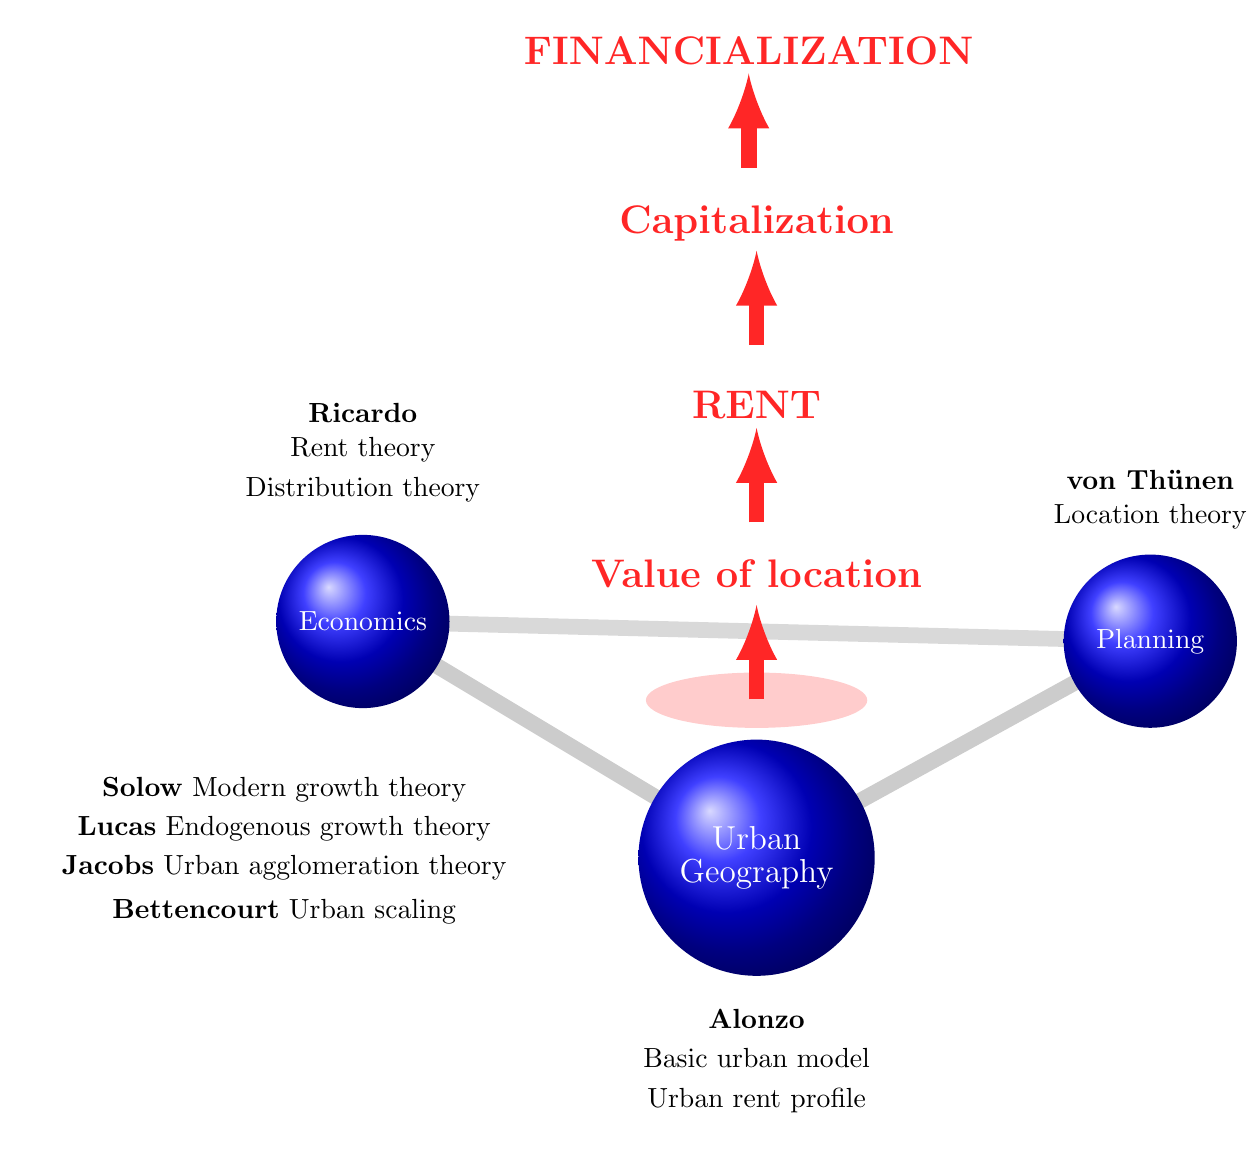
\begin{tikzpicture}{scale=.5}
% Find color for ball. Stop line short of node
\coordinate (planning) at (5,.75); % Preface
\coordinate (economics) at (-5,1); 
\coordinate (Ricardo) at (-5,1.4);
\coordinate (Solow) at (-6,1.25);
\coordinate (geography) at (0,-2); % History
\coordinate (finance) at (0,5); 

\draw [line width=2mm, black!15, ] (planning)--(economics);
\draw [line width=2mm, black!20, ] (geography)--(economics);
\draw [line width=2mm, black!20, ] (geography)--(planning);
%\draw [line width=2mm, black!25, ] (geography)--(finance);
%\draw [line width=2mm, black!20, ] (planning)--(finance);
%\draw [line width=2mm, black!20, ] (finance)--(economics);
%color=black!60!red
%\shade [ball color=blue!70] (5,5) circle (1.1cm)node[white] {\textbf{Planning}};
 
\node [circle,shading=ball,  minimum width=2.2cm, white, align=center] (ball) at (planning) {Planning};
\node [circle, shading=ball, minimum width=2.2cm, white, align=center] (ball) at (economics) {Economics};
\node [circle,shading=ball, minimum width=3cm, white, align=center] (ball) at (geography)[text width=2cm] {\large Urban \\ Geography};
%\node [circle, shading=ball, minimum width=2.4cm, white, align=center] (ball) at (finance)[text width=2cm] {Finance};
%\node at (-.3,-.1) [red] {\Large \textbf{RENT}};

\node at (planning) [above=1.8cm] {\textbf{von Th\"unen}};
\node at (planning) [above=1.3cm] {Location theory};

\node at (Ricardo) [above=2cm,]   {\textbf{Ricardo}};
\node at (Ricardo) [above=1.5cm] {Rent theory};
\node at (Ricardo) [above=1.0cm] {Distribution theory};

% \node at (Solow) [below=1.6cm, align=left] {\textbf{Solow:}};
\node at (Solow) [below=2.1cm, align=left] {\textbf{Solow} Modern growth theory};
\node at (Solow) [below=2.6cm, align=left] {\textbf{Lucas} Endogenous growth theory};
\node at (Solow) [below=3.1cm, align=left] {\textbf{Jacobs} Urban agglomeration theory};
\node at (Solow) [below=3.65cm, align=left] {\textbf{Bettencourt} Urban scaling};

\node at (geography) [below=1.8cm] {\textbf{Alonzo}};
\node at (geography) [below=2.3cm] {Basic urban model};
\node at (geography) [below=2.8cm] {Urban rent profile};
%\node [circle, shading=ball, minimum width=2.4cm, white, align=center] (ball) at (finance)[text width=2cm] {Finance};

\fill[red!20] (0,0) ellipse (40pt and 10pt);
%\node[red]at (1.2,0) {\large SPACE};
\begin{scope}[shift={(0,-.34)}]
\draw [line width=2mm, red!85, -latex ] (-.1, 7.1)--++(0,1.2)node[above=-.1] {\Large \textbf{FINANCIALIZATION}};
\draw [line width=2mm, red!85, -latex ] (0, 4.85)--++(0,1.2)node[above=-.1] {\Large \textbf{Capitalization}};
\draw [line width=2mm, red!85, -latex ] (0, 2.6)--++(0,1.2)node[above=-.1] {\Large \textbf{RENT}};
\draw [line width=2mm, red!85, -latex ] (0, .35)--++(0,1.2)node[above] {\Large \textbf{Value of location}};
%\draw [line width=2mm, red!85, -latex ] (0, -2)--++(0,-.8)node[above=-.1]  {\Large \textbf{SPACE}};
\end{scope}
\end{tikzpicture}
    \caption[Linking space and urban rents to the effects of financialization.]{Space and urban rents play a foundational role in urban economics, geography, and planning. We extend the analysis of urban rents to model the effects of financialization.}
    \label{fig-fields}
    \end{figure}


%To model the effects of financialization on wealth distribution, we combine a modern approach to spatial rents with a return to the classical focus on distribution. 
To model the distribution of locational rents in an urban system, we go back to the classical theory of rent. The concept of economic rent was developed by the classical economists of the late eighteenth and early nineteenth centuries to explain how wealth was created and distributed in an agricultural society. David Ricardo \cite{ricardoEssayInfluenceLow1815} elaborated the classical theory of land rent and distribution to explain economies dominated by agricultural production in 1815.
Johann von Th\"unen \cite{vonthunenIsolirteStaatBeziehung1826} produced the first formal treatment of spatial economics and economic geography in 1826. 

Much later, in 1961, William Alonso (and others) \cite{alonsoModelUrbanLand1960} applied the Ricardian and von Th\"unen theory to the urban system, launching modern urban rent theory.  The spatial implications of the classical analysis were brought forward into modern urban theory, but the distributional implications were not. Our work is designed to integrate the two

Since an essential feature of cities is that they grow, we also draw on growth theory that looks at agglomeration effects and scaling laws to account for how distribution is affected by scale.  As Alonso and others were developing urban rent theory, the economist Robert Solow \cite{solowContributionTheoryEconomic1956} proposed a theory of economic growth that set off a flood of work The new field spilled into urban theory and connected with a rich body of work on economic development and the value created in cities, including work by Jacobs \cite{jacobsEconomyCities1969}, Lucas \cite{lucasMechanicsEconomicDevelopment1988}, Bettencourt \cite{bettencourtGrowthInnovationScaling2007}, and others. We draw on this body of work to account for the scaling of productivity with population. We also draw on neoclassical economic theory for its explanations of how the value of production in firms is shared among the owners of various resources. Our work brings these traditions together into an integrated picture that allows us to look at wealth distribution within a spatial model that includes productivity and growth.  

 What has been missing until now is a detailed account of who gets the land rents in the modern urban system. Our contribution is to extend the analysis of urban rents to take into account the effects of financialization, which is fundamentally a distributional process. This is a significant step because, while classical rent theory is the foundation for urban rent theory, the distributional aspects of the classical theory have not been applied. Meanwhile, standard models of financial operations are spaceless. This means the standard models don't relate them to spatial rents.\footnote{%In describing any theory we need to identify the kinds of objects that are theorized. 
 Financial analysis theorizes assets, debts, flows of revenue and costs, and the rates of change or exchange of these quantities over time. These are inherently spaceless because they are accounting entities, independent of location. It matters where a worker or a farm is, but it does not matter where and dollar or a rouble is in the same way.} 
 
 Our solution is to explicitly embed the normally spaceless analysis of investment decisions in a spatial model with locational rents. 
We bring together three theoretical elements: an urban spatial model,  an agglomeration-augmented model of wealth production in urban centers, and a financialized land market model built on top of the first two.\ %We incorporate that scaling result into the standard urban model, building of the work of William Alonso and others. 
 We call the combination of the spatial and production models the Alonso-Jacobs model, recognizing the sources of the two elements. 

% The city generates a surplus, and financialization is about capturing surplus. 
The model makes it possible to analyze the potential macro effects of financial capital capturing spatial urban rents. Our focus is on changes in who captures these rents, and how that affects the productivity of the city. The distribution of locational rents, we believe, goes some distance to explaining core social issues like class structure, inequality, and political power.

\section{Modelling financialization of urban housing markets}
{\color{red}
The goal of building our model is to bring the aforementioned elements into one combined model that allows us to explore the distributional effects of the financialization of a housing market. 
%{\color{red} To do this we combine }

We generate the value created in city with a model of firm production that generates an equilibrium wage target. A wage offer is passed to  a spatial model of the city where agents choose whether or not to participate base on the wage, transportation costs, and their location. The model generates Ricardian rents which accrue to property owners. Owners and rent seeking investor agents compete in the housing market for the rents. % understand how that value is distributed through property markets, and study how the entry of financial capital changes the distribution of land ownership. 

We develop a model with three components: an urban housing market, a financialization process, and an urban production system.} The housing market sub-model distributes the ownership of the housing stock that comes up for sale in each period based on bids. % Both new entrants to the labour pool and financial investors can bid. If a new entrant fails to buy  housing that agent becomes a renter. 
The market determines the price for each unit. The price may depart from the market value of the services that each unit provides, providing the opportunity for speculative gains. Finally, the financial model determines the size of bids for investors based on the availability of capital and estimates of rental income and capital gains.

%the\cite{alonsoTheoryUrbanLand1960}, calling the combined sub-model the \gls{Alonso-Jacobs cycle} because there is a positive feedback between population size and wages. This feedback loop will be vulnerable if financialization extracts the new wealth generated by agglomeration effects, reducing wage growth and therefore the ability of the city to grow, because wage growth is what drives population growth and further agglomeration. The green boxes in the figure represent the theoretical justification of the primary simplifications in the model. 

\begin{figure}[!ht]
\centering
\includegraphics[scale=.20]{fig/flow-impacts.png}
\caption[The housing market component of the model.]{The housing market component. Financialization affects both the allocation of housing and its allocation of rents.}
\label{fig-impacts}
\end{figure}

Figure~\ref{fig-impacts} shows the logic of the first component, the housing market model.
It shows two primary effects financialization has on the housing market: how it allocates
the housing stock, and how it allocates the \glspl{rent} generated by the urban system. 
The first effect of financialization, on housing allocation, arises because tenants replace owners. While owner-occupiers share in the growing land rents generated by urban agglomeration effects, tenants do not. As a result, a declining fraction of urban residents accumulate capital through their participation in the housing market, and therefore fewer enter the class of workers with both wage and capital income defined by John Roemer \cite{roemerGeneralTheoryExploitation1982}. 

The second effect of financialization on the market is in the allocation of spatial rents, generated in part by the growing productivity of cities. Rents generated by the \gls{agglomeration} economies in the urban system are diverted to largely non-resident owners, away from investment in local production or amenities, as tenants replace owner-occupiers.

\begin{figure}[!ht]
\centering
\includegraphics[scale=.20]{fig/flow-financialization.png}
\caption[The financialization component of the model.]{The financialization component. There is a feedback loop in which new investors drive up demand and thus drive up prices.}
\label{fig-financial-cycle}
\end{figure}

Figure~\ref{fig-financial-cycle} illustrates the second component of our model, the financialization process. We develop an explicit model of investor behaviour to explain the market decisions of buyers and the role of financial capital. %The key observation is that 
Investors enter the housing market and, in doing so, they drive up prices by increasing total demand. The rising price generates an expectation of capital gains, which enter the investors' calculations. Investors have, as research shows, better access to capital than most new entrants to the housing market. When the financial sector, the bank in the model, makes more capital available, the pattern of ownership shifts, as illustrated above.

Figure~\ref{fig-alonso-jacobs-cycle} illustrates the third component, the feedback between population and productivity. The green blocks represent the theory linking the relevant variables.  On the lower right, ``Scaling'' refers to the literature on agglomeration effects. On the upper right, neoclassical distribution theory provides a model linking productivity with wages.  On the left, the bid rent function links wages and population.


\begin{figure}[!ht]
\centering
\includegraphics[scale=.2]{fig/flow_Alonzo-Jacobs_cycle.png}
\caption[Production system.]{The production system component, incorporating the urban scaling of wealth in the urban spatial model. We refer to this coupling of two different equations as the Alonso-Jacobs cycle.}
\label{fig-alonso-jacobs-cycle}
\end{figure}

A fundamental feature in recent empirical work on scaling laws is the persistent relationship between population and productivity. The productivity of cities increases superlinearly with population. Cities are the locus of a positive feedback loop with rising populations raising productivity, and rising productivity attracting more people and resources, a theoretical argument associated with the work of Jane Jacobs \cite{jacobsEconomyCities1969}, with strong empirical support from recent work on the scaling of urban productivity  \cite{bettencourtGrowthInnovationScaling2007, bettencourtOriginsScalingCities2013, dongUnderstandingMesoscopicScaling2020, loboUrbanScalingProduction2013}.


Combining these three components, we have an extended theory of urban rent built on a foundation of theory that goes back to the \gls{classical economics} around the beginning of the 19$^{th}$ century and incorporating modern growth theory and modern urban theory. 

The resulting model suggests two basic hypotheses:
\begin{enumerate}
    \item Financialization of the housing market will result in the tenantization of the urban middle class as financial capital acquires more of the housing stock. % vs decline of the urban middle class
    \item Financialization of the housing market will result in reduced growth of urban productivity as the flow of rents is diverted from real investment to the financial sector.
\end{enumerate} 
 
\section{Contributions}
The overall goal is to provide a theory of the relationship between financialization and urban productivity. The main contributions towards achieving this goal are:
\begin{enumerate}
    \item  Incorporating \gls{classical rent theory} into an \gls{agent-based} urban model. This requires modelling how \gls{Ricardian rent theory}, a theory of distribution based on an agricultural economy, applies in an economy driven by human capital \gls{agglomeration} effects within the urban system. 

    \item Allowing the creation and distribution of rents to influence urban growth, productivity and population structure. This requires articulating the links between the wealth production of cities and how the urban system evolves.

    \item Incorporating current research on \gls{urban scaling} into the core spatial urban model.  This requires drawing on empirical work to formalize the scaling relationship, which embeds productivity in an urban model. 

    \item Constructing an urban \gls{agent-based model} that is consistent with {neoclassical growth theory}. We show how the neoclassical framework can be implemented in the agent-based framework, and make a case for the usefulness of the approach in linking urban rents and productivity. 

    \item Integrating \gls{financial capital} into a standard spatial model of the urban system, making an explicitly spatial model of the financial structures, which have traditionally been formalized in a spaceless way.
    
    \item Integrating financial capital into an \gls{overlapping generations} population model of the urban system and articulating the movement of financial capital though the urban land market. 
    
    \item Using an agent-based model to examine how financial markets impact urban \glspl{land market}, producing a formal simulation model that illustrates the process of housing financialization. 

    % \item Testing for \gls{hysteresis} resulting from the business cycle in the urban system and exploring the \gls{resilience} implication's of the core spatial economic model.

    \item Building a model that can be easily extended to explore a range of issues, and used to evaluate policy options. The model combines clear and explicit theoretical assumptions with careful and transparent implementation of the logic. We have taken care to allow for both theoretical and policy-relevant extensions in the simulation,  building a base model that aims to be as simple as something like Alonso's urban model \cite{alonsoLocationLandUse1964}, but simulates the relevant system features and can incorporate a range of intervention types. 
\end{enumerate}


\section{Document overview}
There are two parts in the dissertation. Part~\ref{part-background} gives the background and introduces the theoretical framework for the analysis, linking financialization with classical rent theory, neoclassical production theory, neoclassical growth theory, the scaling literature, and urban spatial models. 

\begin{enumerate}
    \item Chapter~\ref{chapter-financialization} discusses finacialization.

    \item Chapter~\ref{chapter-rent} reviews the literature on rent and introduces an an approach % doest hat fix it? develops an approach ***E  i FIND THIS PHRASING A  BIT AMBIGUOUS. ARE YOU DESCRIBING HOW YOU DEVELOPED THE APPROACH OR LAYING OUT THE APPROACH??? suited to the analysis for this work.

    \item Chapter~\ref{chapter-space} develops the urban model of space drawing on the basic Alonso model.

    \item Chapter~\ref{chapter-growth} introduces growth theory, showing how our model is directly connected with this broad collection of linked theories. 

    \item Finally, Chapter~\ref{chapter-tramsmission} discusses the potential feedback by which financialization, can affect the productivity of the urban system. %mechanisms for the transmission of the immediate effects of financialization to city productivity and growth.
\end{enumerate}
 
\noindent Part~\ref{part-model} describes the methodology, model, and results.

\begin{enumerate}
    \item Chapter~\ref{chapter-methodology} introduces the methodology for the approach. 

    \item Chapter~\ref{chapter-model} details the model of the illustrative agent-based model of the urban system. This model has three  parts: first, a production function, modelling how urban regions generate wealth,  second, a model of an urban housing market, and, finally, a financial sector that can participate in the market. 
% \end{enumerate}

% \noindent Part~\ref{part-analysis} develops the analysis, implications, and extensions for the base firm and housing market model.

% \begin{enumerate}
    \item Chapter~\ref{chapter-results} introduces the results, including the
    %\item Chapter~\ref{chapter-ownership} shows the 
    basic ownership result %.
    %\item Chapter~\ref{chapter-tramsmission} experiments  with the base model, and an extension to consider spillover productivity effects.
    % \item Chapter~\ref{chapter-extensions} introduces several extensions including amenity and transportation.
    % , and an extension to include amenity, respectively. 
    The experiments explore the static and dynamic effects of interventions in each case. % including our conclusions about the resilience of our social structure in the face of financialization.
    % \item \item Finally, Chapter~\ref{chapter-conclusions} draws conclusions from the work.
\end{enumerate}

\noindent Part~\ref{part-conclusions} %sketches future work and 
concludes. 

\begin{enumerate}
    \item Chapter~\ref{appendix-future-work} discusses future work. 
    \item Finally, Chapter~\ref{chapter-conclusions} draws conclusions from the work.
\end{enumerate}



% ADD BACK IN
% \begin{figure}
% \centering
%  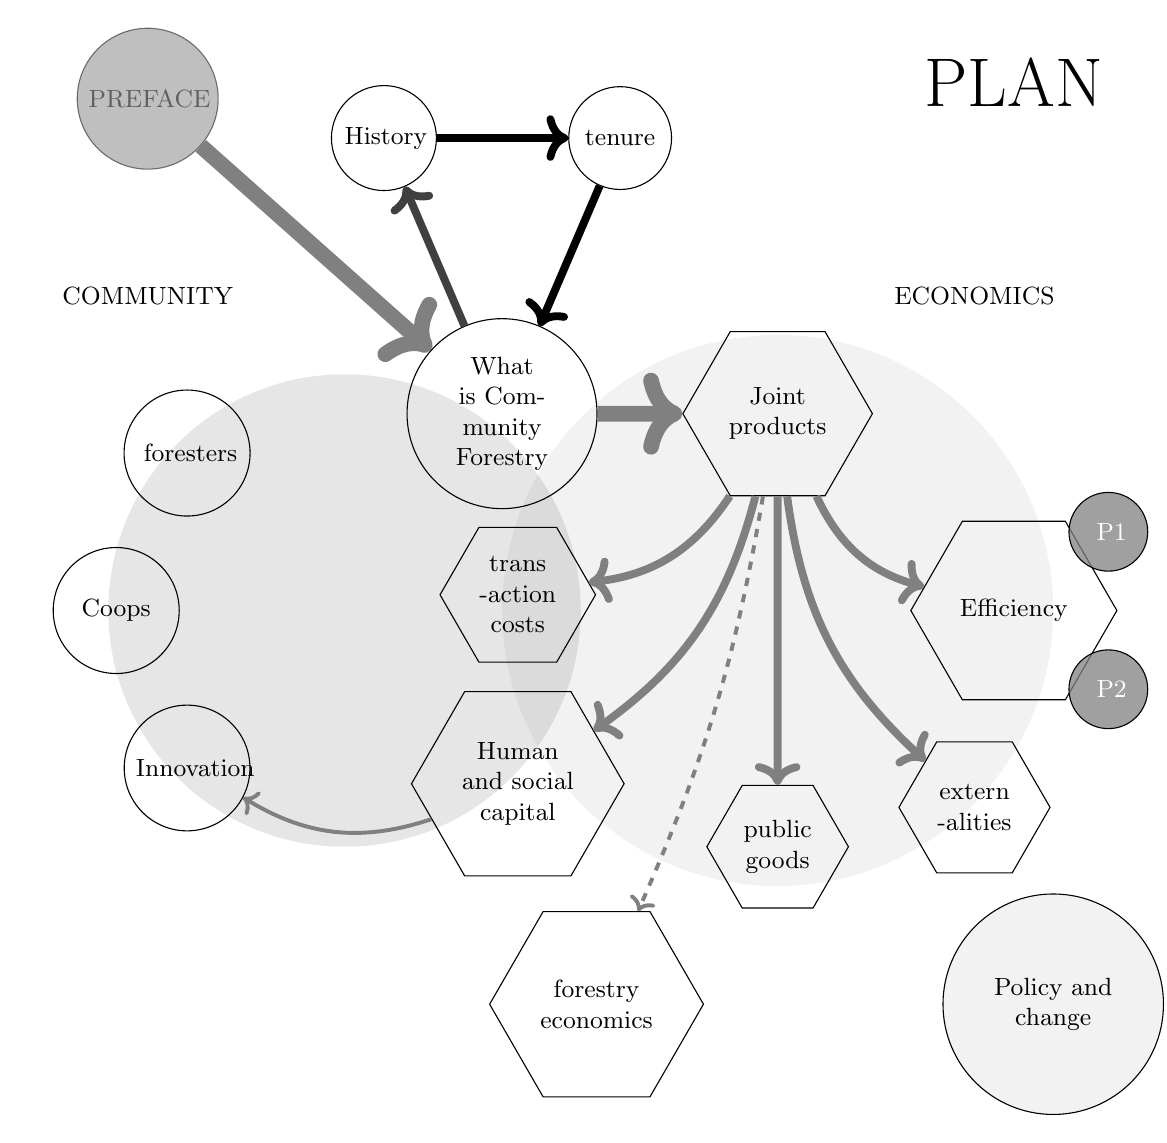
\begin{tikzpicture}%[scale=.8]
    \tikzstyle{every node}=[font=\small]
%\draw[help lines,step=.5] (0,-11) grid (11,11);

\coordinate (aa) at (-1.5,7.5);%PREFACE
\coordinate (a) at (-1,10);%
 \coordinate (b) at (1.5,7); %history
\coordinate (c) at (6,10); %
\coordinate (d) at (9,9);%
\coordinate (ee) at (-4,7);%
  \coordinate (e) at (-1.5,5); %Community label
\coordinate (f) at (9.5,7.7); %???    PLAN
\coordinate (g) at (9,5); %Economics label
\coordinate (h) at (4.5,7);%tenure
\coordinate (ii) at (-4,4);%
   \coordinate (i) at (1,4);  
\coordinate (j) at (3,3.5);%whatis
\coordinate (k) at (6,4);%
 \coordinate (l) at (6.5,3.5);%joint
\coordinate (mm) at (-1.9,1);%coops
 \coordinate (m) at (1,1);%community grey circle
  \coordinate (n) at (3,1); %
  \coordinate (o) at (9.5,1); %efficiency
				 \coordinate (oo) at (6.5,1);%
				  \coordinate (o1) at (10.7,2);	 \coordinate (o2) at (10.7,0);%Propositions
\coordinate (p) at (9,-1.5);%externalities
				
\coordinate (qq) at (-4,-2);
\coordinate (q) at (-1,-1);%innovation
 \coordinate (r) at (3.2,1.2);%trans
  \coordinate (s) at (3.2,-1.2);%capital
 \coordinate (t) at (6.5,-2);%pubgoods
\coordinate (AA) at (-2,-5);%
 \coordinate (A) at (1,-5);%
\coordinate (B) at (3.7,-4); %
\coordinate (C) at (4.2,-4);%forestryEC
\coordinate (D) at (-1,3);%foresters
\coordinate (EE) at (-1,-8); \coordinate (E) at (1,-8); \coordinate (F) at (3,-8); \coordinate (G) at (6,-8); \coordinate (H) at (10,-4);%Policy
\coordinate (II) at (-4,-11);  \coordinate (I) at (1,-11); \coordinate (J) at (3,-11); \coordinate (K) at (6,-11); \coordinate (L) at (10,-11);
%\coordinate (M) at (coordinate); \coordinate (N) at (coordinate); \coordinate (O) at (coordinate); \coordinate (P) at (coordinate);
%\coordinate (Q) at (coordinate); \coordinate (R) at (coordinate); \coordinate (S) at (coordinate); \coordinate (T) at (coordinate);
% \fill[red, fill opacity=.8] (0,0) circle (4cm);
\fill [gray, fill opacity=0.2] (m) node [text width=2cm, black, opacity=1] 				(community)	{} circle (3cm);
\fill [gray, fill opacity=0.1] (oo)  node [text width=2cm, align=left, black, opacity=1] 		(econ) {} circle (3.5cm);
\node at (e) [ ] 		(comLtabel) {COMMUNITY};
\node at (g) [ ] 		(ecLabel) {ECONOMICS};
				%\draw (0,3.2,1) node [text width=1.5cm, text centered] {$Economics$};
			%\draw [fill=red, fill opacity=0.3]  (aa) node [ text width=2cm, black, opacity=1] 									(preface)		{PREFACE: Why, claims} circle (1.4cm);
\node [circle, draw,  fill=gray, opacity=.5,, text width=1.5cm] at			 (aa) 		(preface)		{PREFACE};
\node [] at			 (f) 		(plan)		{\Huge PLAN};
			%\draw [fill=blue, fill opacity=0.35] (b)node [text width=2cm, align=center, black, opacity=1] 			(history){History: New is Old} circle (1.2cm);
\node[circle, draw, text width=1cm, align=center, black, opacity=1]at 	(b)(history){History} ;
			%\draw [fill=pink, fill opacity=0.5] 		(h) node [text width=2cm, black, opacity=1] 								(tenure) 	{\color{black}tenure} circle (1.2cm);
\node[circle, draw,  text width=1cm, align=center, black] at 				(h) (tenure) 	{tenure} ;
\node[circle, draw,  text width=1.5cm, align=center]at							 (j) (whatis) 	{\color{black}What is Community Forestry} ;
\node[regular polygon, regular polygon sides=6, draw, align=center]at (l) (joint) 	{\color{black}Joint\\  products} ;


%\node[circle, draw,  text width=2cm, align=center]at (h) (tenure) 	{\color{black}tenure} ;

%\draw [fill=red, fill opacity=0.5] (j) node [text width=2cm, black, opacity=1] 												(whatis)		{What is Community Forestry}circle (1.4cm);
%\draw [fill=orange, fill opacity=0.5] 	(l) node [text width=2cm, black, text opacity=1] 	               		(joint)	{Joint products}											 circle (1.2cm);
%\draw [fill=green, fill opacity=0] (1,5)node [text width=2cm,red, opacity=1] {Policy and change} circle (1.4cm);
%\draw (q) node [text width=1.3cm, align=center, black, opacity=1] (small)	 {Innovation} circle (1.1cm);
\node[circle, draw,  text width=1.3cm, align=center] at							 (q) (small)	 {Innovation} ;

\draw 	(mm) node [text width=1.3cm, align=center, black, opacity=1] 	(coops) 	{Coops} circle (.8cm);
%\draw [fill=orange, fill opacity=0.5] 	(s) node [text width=2cm,  align=center, black, text opacity=1] (capital) {Human \\and social \\capital} circle (1.2cm);
\node[regular polygon, regular polygon sides=6, draw, align=center] at (s) (capital) {Human \\and social \\capital} ;
%\draw [fill=gray, fill opacity=0.5] 			(o) node [text width=2cm, black, text opacity=1] 						(efficiency)	{Efficiency} circle (1.2cm);
\node[regular polygon, regular polygon sides=6, draw, align=center] at (o) (efficiency)	{Efficiency};
\draw [fill=gray, fill opacity=0.75] (o1) node [text width=.3cm, white, text opacity=1] (	P1)  {P1} 		circle (.5cm);
\draw [fill=gray, fill opacity=0.75] (o2) node [text width=.3cm, white, text opacity=1] (P2) {P2} 			circle (.5cm);

%\draw [fill=orange, fill opacity=0.5] (p) node [text width=2cm, black, opacity=1]					(externalities)	 {externalities} 			circle (1.2cm);
%\draw [fill=orange, fill opacity=0.5] (t)node [text width=2cm, align=center, black, opacity=1] (pubgoods) {public goods} 		circle (1.4cm);
%\draw [fill=orange, fill opacity=0.5] (r) node [text width=2cm, black, opacity=1] 							(trans)	{transaction costs} 		circle (1.1cm);
\node[regular polygon, regular polygon sides=6, draw, align=center] at (p) (externalities)	 {extern\\-alities};
\node[regular polygon, regular polygon sides=6, draw, align=center] at (t) (pubgoods) {public\\ goods} ;
\node[regular polygon, regular polygon sides=6, draw, align=center] at (r) (trans)	{trans\\ -action\\ costs};



%\draw [fill=yellow, fill opacity=0.15] 	(C) node [text width=2cm, black, opacity=1] 							(forestryEC){forestry \\ economics} circle (1.4cm);
\node[regular polygon, regular polygon sides=6, draw, align=center, fill=gray!.25] at (C) (forestryEC){forestry \\ economics};
\draw [] 	(D) node [text width=1.1cm, black, opacity=1] 							(foresters)	{foresters} circle (.8cm);

  %%%%%JOINT PRODUCTS  AND TRANSACTION COSTS
%\draw [fill=orange, fill opacity=0.5] (G) node [text width=2cm, black, opacity=1] 								{efficiency} circle (1.4cm);
  %%%%%%%%%%%%%%%%%%%%  POLICY CHANGE
\draw [fill=gray, fill opacity=0.1] 		(H)    node [text width=2cm, align=center, opacity=1] 										{Policy and change} circle (1.4cm);
%ADDITIONAL TOPICS
%\draw (J) node [text width=6cm, text centered] {Economic Development };
%\draw ()--();

\draw [gray, line width=2mm,-> ](preface)--(whatis);
\draw  [darkgray, line width=1mm,<- ](history)--(whatis);
\draw  [black, line width=1mm,-> ](tenure)--(whatis);
\draw  [black, line width=1mm,-> ](history)--(tenure);

\draw [gray, line width=2mm,-> ](whatis)--(joint);
\draw [gray, line width=1mm,-> ](joint) to [bend right=25](efficiency);
\draw  [gray, line width=1mm,-> ] (joint) to [bend left=20](capital);
\draw [gray, line width=1mm,-> ](joint) to [bend right=20](externalities);
\draw [gray, line width=1mm,-> ](joint) to [bend left=25](trans);
\draw  [gray, line width=1mm,-> ](joint)->(pubgoods);
\draw  [gray, line width=.5mm,-> ](capital) to[bend left=25](small);
\draw  [gray, line width=.5mm,-> ,dashed](joint) to[bend left=7](forestryEC);
\end{tikzpicture} 
% \caption{Document overview.}
% \label{fig-community-forestry}
% \end{figure}

% \bibliographystyle{plainnat} % or try abbrvnat or unsrtnat
% \bibliography{jmp.bib} % refers to example.bib
% % \printbibliography
% % javascript:void(0);

%==================================================================
\chapter{Methodology} \label{chapter-methodology}
%==================================================================
\epigraph{The choice, then, is not whether to build models; it's whether to build explicit ones.}{Joshua M. Epstein \cite{epsteinWhyModel2008}}
%\epigraph{One of the very important components in the urban and agricultural land use model is the so-called \gls{bid-rent curve}. Regional and urban economists, city planners, and economic geographers have used this curve extensively as an analytical device.}{Yeung-Nan Shieh \cite{shiehWilhelmLaunhardtBidRent2004}}

% CITE DEREKS PIECE ON MODELS AS BUILDING BLOCKS---MODELS AS eAGOOD PARTS---CITE TERRY'S THESIS---SHOULD DO WHAT IT DOES HOW IT DOES, BUT ABILITY TO COARSE GRAIN- ACTUALLY SWITCH BETWEEN THESE TWO PIECES-  WITH AN EQUILIBRIUM ASSUMPTION AS THE BRIDGE.

% \epigraph{One of the very important components in the urban and agricultural land use model is the so-called \gls{bid-rent curve}. Regional and urban economists, city planners, and economic geographers have used this curve extensively as an analytical device.}{Yeung-Nan Shieh \cite{shiehWilhelmLaunhardtBidRent2004}}
 % \epigraph{It may be tempting to specify an aggregate production function that directly relates primary factors to final output, as is customary in much economic analysis. This standard simplification is often inadequate, however, because cities are characterized by increasing returns to scale, and how psuch increasing returns are generated has potentially important policy implications. In particular, detailed assumptions are needed about rlabor, the nature of products, the production function of individual firms, the input-output structure that links firms, and how firms compete.}{Spence et al. \cite{spenceUrbanizationGrowth2009}}
 % TODO ADD THE PURPOSES OF MODELLING NOTE TO eDISCUSSION OF HOW  WE ARE USING ABMS

% SUMMARIZE: WE ARE MODELLING THE RELATIONSHIP BETWEEN FINANCIALIZATION AS sentsGRAWTH VALUE CAPTURES AND PRODUCTION IN CITIES TO DO THIS WE  BUILD ABM

% ROOTED IN NEOCLASSICAL AND CLASICAL (MOVE THAT SECTION UP??) 

% ABM ADDS WHAT?? GO INTO HISTORY OF ABM AND THEN HOW YOU USE IT TO MODEL THAT ASPECTS YOU HAVE INTRODUCED IN EARLIAR SECTIONS


So far, we have introduced the theoretical frameworks for understanding locational value, the structure of the city and how productivity scales with wealth. In the following chapters, we introduce a model that brings these together to explore the effects of financialization on the urban system. In this chapter, we consider some of the broader methodological issues involved. Section~\ref{sec-purpose} considers the general purpose and strategy of modelling. %: what is the purpose of modelling? what claims does it allow about the outside world? and what is the modelling strategy?
Section~\ref{sec-types} explains what type of model we use and why,  describing how we integrate agent-based modelling and equilibrium approaches in the model.   % in particular what is the underlying paradigm for modelling each component, what are the agents, what simplifications are justified, what uses are made of equilibrium reasoning? 
% Section~\ref{sec-other} describes our approach to several methodological matters specific to our project and the final section {\color{red} does what?}

\section{Purpose and strategy}\label{sec-purpose}
% The goal of modelling in general is to have an accessible and useful description of reality.  

The purpose of the model is its goal, and the strategy is the means by which it seeks to achieve its goal. To define our purpose and strategy, we are guided by the guidelines laid out by Mader et al. for the properties of a good model \cite{maderConstructionVerificationModels2007}. % They emphasize that it should have a clearly specified object of modelling and a clearly specified purpose. They go on to 
% They list the following epistemological criteria, 
They argue that a model should be: 
\begin{enumerate}   
\item  Truthful. The model has to represent the relevant behaviour of the system. % we are describing.
\item  Complete. It must include necessary features of the system.
\item Simple. It must be possible to verify and debug the model.
\item Understandable. Elements should be clearly described or derived and documented.
\item  Traceable.  It should be obvious what elements of the artifact went into which design decision and are reflected at which point in the model.
\item  And finally, efficiently constructable and maintainable.
\end{enumerate}

Frits Vaandrager %\cite{} %(2010 \url{http://www.cs.ru.nl/~fvaan/PV/what_is_a_good_model.html})   
augment their list to produce the following.\footnote{Vaandrager's useful list appears on his faculty webpage at the Institute for Computing and Information Sciences, Raboud University \url{http://www.cs.ru.nl/~fvaan/PV/what_is_a_good_model.html}. % I have not found it published elsewhere, but  
} A good model: \begin{enumerate}
     \item Has a clearly specified object of modelling.
     \item Has a clearly specified purpose.
     \item Is traceable: each structural element of a model either (1) corresponds to an aspect of the object of modelling, or (2) encodes some implicit domain knowledge, or (3) encodes some additional assumption.
     \item Is truthful: relevant properties of the model should also hold for the object of modelling.
     \item Is simple (but not too simple).
     \item Is extensible and reusable.
     \item Has been designed and encoded for interoperability and sharing of semantics.
 \end{enumerate}
These principles inform the purpose and strategy of our model.

\subsection{Model purpose}

Edmonds et al. lay out seven purposes of modelling \cite{edmondsDifferentModellingPurposes2019}. These range from prediction of new data and explanation of patterns in the world, to analogy that merely illustrates some phenomena informally. % Following Epstein who proposed sixteen reasons in addition to prediction for modelling  \cite{epsteinWhyModel2008},  
One of the purposes they identify is \gls{theoretical exposition}, which means the purpose is to explore the relationships between variables in the model. This is the purpose of our model. % The mechanisms in the model display. 
While it would require further empirical work to make specific claims about the outside world, 
% whether explanatory or predictive, % Thia does not make it possible to make claims about 
the  model can illustrate relationships and give insight into the implications of theory. 

\subsection{Model strategy}
%Given the purpose, we must select a strategy as a means to achieve that purpose.  
%  Model strategy is the means by which the model purpose is achieved. %In addition to modelling purpose, there is modelling strategy, 
A common approach to strategy is to follow principles or rules of thumb suited to the purpose of the model. % that guide the modelling. % work. % practice. 
%is With a model built for theoretical exposition, the challenge is to systematically explore the relationship between parameters, % show the results, and % qualify any results, making and make clear the limitations of the model. 
A model designed for theoretical exposition  
% A model built for theoretical exposition 
is built to illustrate the implications of theory, not to establish that theory applies in any given situation beyond the model. Our strategy thus has two aspects. % focuses on two things. % seeks to achieve two things. % has two features.
% With theoretical exposition we 
% To achieve aims specific to the purpose of theoretical exposition, we focus on two things. 
% The purpose of our model is theoretical exposition, so our strategy is designed to achieve aims specific to that purpose. 
Firstly, to understand the implications of theory, we remove elements that are not central to understanding the central theoretical questions. Secondly, since we are not attempting to make predictions, 
we focus on patterns and qualitative relationships rather than quantitative values. Our strategy is thus to keep the model simple and descriptive. Edmonds et al. use the acronyms KISS, `keep it simple stupid,' and KIDS, `keep it descriptive stupid' \cite{edmondsDifferentModellingPurposes2019}.

% \subsection{Applying the principles}
% Since simplicity is key to achieving these goals, % That leads us to a long list features of real urban systems that 
We intentionally leave features out of our model to focus attention on the features that matter most to understanding how financialization captures the value produced in cities. We have two basic propositions:
\begin{enumerate}
    \item Financialization of the urban housing stock extracts wealth produced by urban agglomeration effects. 
    % \item Financialization of the urban housing stock changes the class structure of urban society. 
    \item Financialization of the urban housing stock can limit urban productivity growth. 
\end{enumerate}
% Each  of these represents a high-level and general proposition. 
In considering whether to add a feature to the model, we ask: % varying housing density for example, we ask: 
\begin{enumerate}
    \item Is it necessary to demonstrate the principle? 
    \item Would incorporating it result in falsifying our result?
    \item Would incorporating it result in a qualitative difference in our result?
    \item Would incorporating it result in clarifying our result?
   % \item can it be added at a later point to get more neuanced results? 
\end{enumerate}

For example, we need to model how firms set the urban wage and how land markets distribute surplus value to understand the relationship between financialization and the housing market. % production in the urban system. 
 % It should be clear that, 
However, while varying housing density across our model urban system is technically straightforward, it is not necessary to explore or demonstrate any of our three propositions. Including density variation would not undermine our results nor clarify them. % It is simply not useful to incorporate this feature in our model. 
We can say the same about other extensions discussed in Chapter~\ref{appendix-future-work} on future work. %For instance: 
%\begin{enumerate}
  %  \item Adding a detailed production sector with multiple firms. 
   % \item Adding a detailed labour market.
    %\item Adding households of different sizes.
    %\item Adding an income distribution. 
    %\item Adding a range of distinct occupations.
    %\item Incorporating more complex lifestyle choices.
    %\item Articulating the transmission mechanism from productivity to wages and from wages to population. 
    %\item Incorporating building costs. 
    %\item Adding developers.
    %\item And including zoning regulations.
%\end{enumerate}
Those extensions are interesting and would add fine-grained detail to our understanding of how the effects of the financialization of the housing market are distributed, but none of them are essential to exploring the basic relationship. % is likely to affect the qualitative results or make our argument easier to grasp. 
% While making it 
% In the thesis, we have described a stylized model to  establish how the urban system generates rents. Even with its simplifications, the model can describe key features of urban structure and urban history, and addres the core hypotheses.   %In this section, we illustrate some of the insights supported by the model. 
% Extensions can incorporate variations in wages, density, transportation costs, preference, and even building technology and codes. The limitations of the simple, continuous, equilibrium-based versions described above can be overcome using agent-based models to model the evolution of complex and much more realistic urban systems. 

% Our core question in this thesis is about the effects of financialization capturing the value produced as cities grow. We have combined these  approaches to bring together the two pieces you need to understand the financialized capture of the value of the urban system: a model of the urban system and a model of the mechanism by which they capture it. 

% None of these represent methodological transgressions although the combinations may be unusual. 
% The methodological questions that this combination raise are interesting and we get additional insight into the financialization of housing markets by examining them further.

% We begin by reviewing the modeling paradigms, then discuss in some detail the relationship between analytic neoclasical economic analysis and agent-based modelling, how we've integrated the two and why we believe this is a powerful technique for the tendencies inherent in agent-based models, and in particular in understanding the long term distributional questions. 


\section{Types of models}\label{sec-types}
We combine two distinct approaches to modelling social systems: agent-based techniques and equilibrium reasoning. 
Where agent-based models describe behaviours and observe the outcome of the behaviours computationally, most economic modelling is built around equilibrium conditions that are identified \textit{a priori}. Agent-based modelling and equilibrium analysis are complementary, however, and we employ both. We combine a spatially explicit agent-based land market model with equilibrium assumptions about rent levels and an equation-based model of urban production. We employ equilibrium arguments to get clear inputs for the \gls{ABM} from the peripheral models, where there is a great deal of existing theory about how that part of the system should behave.\footnote{Combining agent-based models with components represented as systems of equations is an established approach to modelling:``\dots in an agent model, physical subsystems can be represented naturally using systems of differential equations (e.g. climate, energy, etc.)  (Chappin, Dijkema and Vries, 2010; Chappin and Dijkema, 2009; Davis et al., 2009; Nikolic, 2009)''  (\cite{chappin_simulating_2011} p 61).} 

\subsection{Agent-based modelling}
Agent-based models employ populations of simple submodels (automata, or agents) \cite{shalizi_methods_2006}. They are part of a wide class of models that incorporate the behaviour of distinct entities and explore the interactions among them. The approach was developed in the 1940's when von Neumann and Ulam introduced cellular automata, a simple form of agent model where agents are typically squares on a grid following rules based only on the state of their neighbours \cite{banksStatisticalChallengesAgentBased2021}.

ABMs have proven effective across a range of domains. Examples of ABMs range from models of Bali's traditional economic and social structure, delays in traffic flow, economic bubbles, 
traditional foraging patterns, % (in the Sugarscape models), 
social segregation, and ecological succession networks, to patterns of poverty and crime \cite{open_agent_based_modeling_consortium_comses_????}. %, _netlogo_????}. 
Recent results from disciplines including physics, biology, anthropology, and economics have built a record of useful empirical results \cite{parkerMultiAgentSystemsSimulation2003, parker_multi-agent_2003, helbing_social_2011-1}. 
These have shown ABMs reliably produce phenomena through simulation that were difficult if not impossible to derive from simpler analytical/closed-form expressions. 
% Related modelling approaches include individual-based models, cellular automata, Ising models of atomic spin, the use of swarm phenomena for modelling fabric or fluid motion, and even finite element analysis and parts of graph theoretic modelling.  
% While the details of implementation differ, common principles and patterns of behaviour appear that in ABMs apply across domains \cite{shalizi_methods_2006}.  

In an \gls{ABM}, agents are defined as having adjustment rules or behaviours that respond to environmental variables.\footnote{Modelling agents with agents are defined as having adjustment rules and behaviours has a long history in economic, going back to the 1838 Cournot duopoly model \cite{cournotRecherchesPrincipesMathematiques1838}, for example, which is analyzed using `reaction functions' which simply describe a firm's optimal response to a second firm's output choice. In Cournot's simple case an equilibrium can be directly computed.} 
Unlike equilibrium approaches common in economic analysis, agent-based modelling commits to using computational methods to mimic the distributed decision-making of complex systems like cities. A program is written that considers each agent sequentially and updates agent and system statuses as it goes. The program is allowed to iterate, and the values of any state variables of interest are recorded at each step. The model may or may not settle into a steady state. As with other modelling approaches, ABMs can be used explore the behaviour of the system by varying individual parameters, and to explore the parameter space using Monte Carlo methods.

%agent-based models replace single equation models of sub-systems with populations of simple submodels (automata, or agents) \cite{shalizi_methods_2006}. 
% Just as a system of equations can produce emergent phenomena, so can subsystems of agents. 
% Emergent phenomena may occur because 
One advantage of beginning with an agent-based model is that we are not imposing linearity, or \textit{a-priori} distributions on the behaviour of agents. In an ABM, agents do not make exactly the same decision at exactly the same time. Decisions and timing depend on the speed of information flows, proximities, and other factors. As a result, suites of agents behave differently than the ``representative agents" typical in economic models \cite{darley_towards_1999, tesfatsion_agent-based_2002}. 
%We employ agent-based methods in modelling the labour and housing market. We allow agents to decide to work if the wage justifies commuting to work at the center.\footnote{In a computationally faster version we compute the distance to the boundary once, rather than having each resident or potential resident decide individually if it is worth entering the urban labour market.} We allow individual worker agents to decide whether to purchase a home and to set their own reservation prices when it comes to selling when they retire. Although we limit the variety of agents in this study, the agent-based modelling approach allows us to introduce continual of agents or whole new classes of agents easily.
 % Imposed assumptions might make the model more tractable, but they have little empirical or theoretical justification. 
By including individuals explicitly, agent-based models offer nuance in exploring the effects of individuals on a system, and the make it possible to study distributional effects, space, and individual differences in a much richer way. The structures that emerge result from assumptions about the decisions of those in the system rather than from assumptions about the behaviour of the system. Agent-based models thus may reveal non-obvious implications of structural changes in particular locations, for particular individuals \cite{darley_towards_1999, happe_agricultural_2004}. 
%cite some of the people who show it can be used for structural change)
% Studying large messy models like these has many of the features of studying real social systems. 
%Where it is helpful, other types of models can be linked with agent-based models or used as subsystems. % 

 %There is a large literature on agent-based models. 

%There are good text books as well. Agent models make it possible to represent phenomenal that are hard to represent otherwise including traffic jam, bubbles and crashes, power law and other fat tail phenomenal, critical transitions

%%%%%%%% (Economics has looked at those areas where the behaviour of many individuals can be reduced. Sociology has looked at those areas where individuals matter. Because of constraints from the (1800s) economics has used math and sociology has not.) ABMs are starting to bring math to social theory. Network theorists and big data people are getting hired both in sociology and and economics for this reason. It is because the math is a different kind of thing.

A challenge with ABMs is that they can be hard to extract meaningful information from. ABMs can be computationally intensive, raising significant problems for analysis since there is so much happening in them. This can make them difficult to use in a practical context \cite{banksStatisticalChallengesAgentBased2021}. % Furthermore, since much of the interest in ABM's lies in system behaviour in response to changes in policy \cite{helbing_social_2011-1}, %integrative design paper 
% questions of observability become central. 
% Raising significant challenges for analysis 
%They thus make it possible to look at the effect of the structural impact of policy makers on real individuals. 
% 
% Of course 
Their complexity is also their strength, however. An advantage is that agent-based models represent the structure of individuals interacting in social systems. % They represent specifically the structures that policy makers engage with: how do actions affect individuals, communities, and societies it affects how people act. It provides the capacity to look at those different levels. % They are process models.
% They provide a natural form for modelling transient and long-term dynamics as individuals interact over time.  %They include interacting individuals so 
They thus make it possible to look at the structural impact of interventions on particular  individuals and in particular contexts. This makes agent-based particularly relevant for policymakers because the can provide a more accurate picture of the whole systems policymakers would be working in.

% Since the system level behaviour comes from the interaction of individuals the model does not need to impose distributions on the outcomes over sets of individuals. The distributions can emerge from the system. 



%\textbf{Agent-based models have a number of advantages:} 
%Maybe include some of these.
%
%* We want to model dynamics
%What are the transient and long term effects? 
%How do the details of what individuals do affect the system. How do the changes in the system affect particular people. Not just what is the mean, but what is the distribution? How does it affect an individual?
%
%* We want to be able to model structural change.
%"Although there are proposed examples of SDs with changing structures (Duggan, 2008), they have not yet matured: in SD the structure of the system is fixed (Yücel, 2010)."
%The other models fix structure.
%
%* There are advantages to process models. 
%It does what we want in the way the system does it.
%
%The cost is that disabragating makes for larger models. They are computationally more intensive and they are more difficult to draw insight from. 
%
%If a simpler model is adequate, a more complex one should not be used. 
%
%This suggest a process model where phenomena that emerge from interacting individuals are modelled as 
%And phenomena represented well by continuos processes are represented in that way (NEwton is many interacting bodies.)
%And where events are modelled using discrete events. 

% This section reviews approaches to models and makes the case that computer models and specifically agent-based computer models are particularly well suited to the problem of understanding how interventions shape social systems.

% "Fundamentally, I'm not sure that agent-based modeling amounts to anything other than object-oriented programming for disaggregated simulations `` \cite{http://vserver1.cscs.lsa.umich.edu/~crshalizi/notebooks/agent-based-modeling.html}

% "Complex  systems models can also serve as stochastic models {\bf Ergodic deterministic systems might as well be stochastic}  Some of them are related to standard, modern stochastic models e.g., {\bf agent-based models are “interacting hidden Markov models” or “dynamic Bayes nets with latent variables}"\cite{Cosma talk on stats complex}


%%%%%%%%%%% FROM PAMPAS DOCUMENTATION 
% "We adopt agent-based modeling as a suitable approach to quantitatively model agricultural systems, their \textbf{structural change}, and endogenous adjustment to policy interventions (Happe et al., 2004). Agent- based modeling is a powerful technique for simulating the actions and interactions of autonomous individuals to \textbf{assess emerging system level patterns} (Gilbert, 2008; North and Macal, 2007). An ABM consists of a collection of autonomous and heterogeneous decision-making entities (agents) interacting with one another and an environment. Agents have \textbf{information} about attributes or state of other agents and the environment, and have access to past and current values of their own state variables (e.g., economic outcomes). Agents make \textbf{decisions} using both prescribed rules nd analytical functions; decisions are based on the information agents have available (Gilbert, 2008). An ABM also includes \textbf{rules} that define the relationship between agents and their environment, and rules that determine \textbf{scheduling} of actions in the model (Parker et al., 2003)."

\begin{figure}
    \centering
  \begin{tikzpicture}[scale=0.6]
\draw[thick,<->] (0,10) node[above]{$Price$}--(0,0)--(10,0) node[right]{$Quantity$};
\node [below left] at (0,0) {$0$};
\node [below] at (5,0) {$Q^*$};
\node [left] at (0,5) {$P^*$};
\draw(1,1)--(9,9) node[right]{$Supply$};
\draw(1,9)--(9,1) node[right]{$Demand$};
\draw[dashed](0,5)--(5,5)--(5,0);
\end{tikzpicture}  
    \caption{A Supply and demand figure}
    \label{fig:SandD}
\end{figure}

\subsection{Equilibrium reasoning }
Economists rely heavily on equilibrium analysis in their study of systems. 
%ADD BACK? stylized fact---appearing data over again and again... toy in real world. distributional effects of urban wealth growing. The ADVANTAGE OF THIS is that iT ENABLE THIS BROAD UNDERSTAND OF HOW PATTERNS PLAY OUTj
%In Economic modelling the most familiar approach is the analysis of systems in equilibrium. 
Under the equilibrium approach, a set of necessary conditions describing the steady state of interest are imposed. This approach produces tractable models that can often be solved explicitly. It % is a productive methodology partly because it 
bypasses the often intractable and complex process of adjustment, focusing on the conditions that must be true if a particular situation is to persist. This tractability was particularly important before computers became widespread.
% ANALAGOUS TO RESILIENCE.

The most familiar example of an equilibrium model is the ubiquitous supply and demand model. A supply and demand model consists of two curves, each describing a functional relationship between two variables, price and quantity. Each curve represents the preferences of a class of agents, and the model explores the combinations that satisfy the behavioural intentions of both classes i.e. are on both curves.  The demand curve, illustrated in figure ~\ref{fig:SandD} visually represents the quantity of a product demanded by potential buyers at each price.  The supply curve is the quantity that suppliers would be willing to sell at each price.  Equilibrium, in this example at the combination  $(Q^*,P^*)$, refers to a state in which the preferences of both agent classes are satisfied. A situation is unlikely to persist if either class of agents is unsatisfied with the combination of price and quantity. The question at the heart of the equilibrium approach is, ``What conditions are necessary if the situation is to be stable?"  In the case of supply and demand, The quantity supplied must equal the quantity demanded, and the price must be the same for both classes.\footnote{Taxes introduce an additional condition that results in different prices for the two sides.} If the two curves can be described mathematically, equilibrium prices and quantities can be derived by solving the two-equation system.


% It is helpful to remember that 
% The approach makes it possible to simplify analysis and understand long run patterns.  The technique evolved before computers made simulations relatively easy. To achieve tractability, it was necessary to limit the number of variables, and independent decision-makers by employing a `representative agent,' i.e. one agent with consistently defined qualities that represents the class of agents.  

% To extend the analysis to dynamic systems, `laws of motion' (adjustment rules) can be added as either difference or differential equations.  Models quickly become challenging with more agents or dynamic processes, and economists, like other modellers, now very often resort to simulation and numerical methods. 


\subsection{Where we use agent-based models and equilibrium reasoning}
We use an agent-based model for the core model of the process of financialization, where we need to understand individual behaviour and distributional effects. % Because our focus is 
%To understand the relationship between financialization in the housing market and the production of value, central housing and financial sub-model using an agent-based model % we use an agent-based model in the central housing and financial sub-model because that is where the processes most interesting for our work happen. 
The agent-based model allows us to explore how patterns of distribution emerge within a spatial system with many agents.

%We draw heavily on existing economic analysis of cities to identify relevant behaviours and parameters. We also employ three key economic equilibrium conditions drawn from the economic literature: locational, labour market, and  housing market equilibrium conditions 

% In a market with any degree of churn, market prices for land should converge on use values, and these will vary systematically with transportation costs. This is an implication of consumer choice theory. The market-based argument allows us to compute land rents from the transportation cost and urban wage premium that drive urban locational decisions. For simplicity, we present the model for the case where individuals have the same preferences, employment opportunities and transportation costs. We can, if and when we apply the model to questions of urban design and inter-individual distribution, easily introduce site-specific and person-specific features.  

%who make decisions at the margin within an agent-based model (ABM) in which agents make periodic choices among a small set of alternatives. 

We use equilibrium approaches to model urban production. There are two reasons for this choice. First, firms can generally adjust much more quickly than the housing market, so it is reasonable to assume that the quickly adjusting variables like price and employment are close to equilibrium values.  Second, we want to drive the central process with a sub-model that is well understood to ensure that results can be explained easily. Nothing prevents us from replacing the sub-model with one with long lags or a different theory of firm behaviour. 

% We use the standard urban firm model which is based on equilibrium analysis to reproduce key features of the urban production system. 

% In the production sector, 
 % equilibrium levels as inputs to the other parts of the model

% HOW

% Equilibrium wage levels are passed to the spatial model where another equilibrium-based calculation is used to determine target population and locational rents. Population feeds back into the agglomeration function with a lag. Agents in the housing investor agents correctly observe the levels of wage and rent that apply for them in each period. 

% Other variables such as interest rates and mortgage requirements are parameters in agent decision-making. Agents use the observed values when they enter the housing market and make bids in response to the wage. They work, save and eventually retire, putting their homes on the market. Investor agents estimate the revenues and capital gains they would earn if they buy available properties, and make bids as well. Sellers accept the highest bid they receive. 

% WHAT ABOUT THE STUFF BELLOW THIS?

% An example of \gls{equilibrium reasoning} is the \Gls{Alonzo model} approach to imposing a locational equilibrium condition, \[U_i(d_k,\dots)=U_j(d_l, \dots),\] where $U_i(d_k,\dots)$ represents agent $i$'s utility at distance $d_k$. The condition says that identical individuals must get the same utility no matter how far they live from the city centre. If that were not the case, individuals would move to a location where they get higher utility. For utility to remain constant as transportation costs rise, some other variable must compensate. In this class of models, the rent charged for the use of land must fall as distance increases. This is an equilibrium condition. 

% Equilibrium locational choice by commuters therefore determines the extent and ultimately population of the city.\footnote{More complex models allow home sizes and lot sizes in the suburbs to increase as well.} Since land value is \gls{capitalize}d rent, land values also decline toward the edge of the city until they are equal to the rural value of the land. An adjustment process that requires people to move to a different location would take a long time to work through the system. Home prices and rents, however, can usually adjust more quickly. % different location would take a long time to work through the system. Prices, however, can adjust much more quickly. 

Our model of firm behaviour uses a single representative firm to determine the wage. This approach does not explicitly model multiple interacting firms but using  equilibrium reasoning here has the advantage of simplicity and being among the most common approaches to modelling production. 
We sacrifice some complexity in this part but the model of production is less central to our model and we get the advantage of connecting the work with standard work on theory of the firm using simple, well-understood models. 
Using a representative firm allows us to focus on the relationship between the scaling of urban productivity and the financialized ownership that can extract that value, which is the core conceptual contribution of this work. 

There is no loss of generality in using a single firm: we are not interested in the structure of the production sector. Because our focus is financialization in the land market, we only require that wages and employment behave as economic theory tells us they should. Our representative firm is a neoclassical profit-maximizer, adjusting employment and capital stock in every period toward the optimal quantities according to the marginalist rules for maximizing profit.  The model is fully extensible and future implementations could replace the equilibrium model of representative firms with a larger agent-based model of interacting firms. Our overall model is sufficiently modular to plug in a different production sector, perhaps to introduce agents or to link to a model developed elsewhere. 


By integrating the agent-based land market model, the equilibrium assumption about rent and the equation-based model of urban production, three pieces which are traditionally studied separately, this work combines elements of classical rent theory and neoclassical distribution theory with agent-based modelling.




\section{Summary}\label{sec-summary}
In this chapter, we have made our solutions to certain high-level modelling questions explicit. We have explained our purpose and strategy in building the model. We then described the type of modelling used for each piece, the use of agents and the role of equilibrium analysis. In our case, the purpose of the model is \gls{theoretical exposition} and we describe our strategy as an attempt to make a model that is simple, extensible, and reusable, while meeting rigorous criteria for good modelling practice. % 

The model type is a blend of agent-based and equilibrium modelling.
In integrating models of the firm, the urban spatial system, the housing market and the financial system,  % which are traditionally studied separately, 
this work combines elements of classical rent theory and neoclassical distribution theory with agent-based modelling.  We have a spatially explicit agent-based land market model, an equilibrium urban rent model, a neoclassical equation-based model of urban production, and a rule-based mortgage provision system.

The work thus draws on a variety of methodologies. % and raises subtle modelling issues. 
We have at each point grounded modelling decisions in established theory and eliminated elements that would add unnecessary complexity, while focusing on building an extensible model that illustrates the relationship between urban production and the capture of rent through land markets.

 % Finally, given our purpose and methodological decisions, we have focused on developing a model that is both simple and descriptive. 



 %ADD BACK WE USE IN TWO PLACE WITH DIFFERENT PURPOSES ...  So in the model we have MODEL OF PRODUCTION LAND MARKET LINK BETWEENTHE AND RENT WHICH IS NOVEL application serves as link between them.



% We identify the classical period loosely as 
% Neoclassical and classical theories are often seen as opposed ideologically, since the classicals 
 % The  opposition in our view is exaggerated. 
% Many  who employ ABMs to analyze urban systems are deeply skeptical of neoclassical assumptions while ignoring the rent;-based distributional analyses of the classicals.

% In ABMs it is often makes sense to simplify models, less for computational reasons then to % The problem of model complexity remains a challenge with ABMs, however, and modellers introduce simplifying assumptions. These are not as a rule needed for the computational model but are helpful in maintaining a focus on the key theme  of the model.  %(ADD distinction between detailed models and detailed explicit models)


% These ideological overlays are not helpful in making choices about how to model. We would argue that ABM modelers who assume mainstream economists actually believe that the neoclassical technique of reasoning based on informed rational agents is based on faith or ideology are mistaken. 
%The neoclassical approach is a modeling technique and a methodological convenience. {\color{red}RESTATE WHAT THE NEOCLASSICAL APPROACH IS FOR CLARITY} %, that is widely used across economics. %, that is valuable when it is used correctly.  
%To the extent that it is limited, its limitations may be explored by making it interoperable with a model that makes it systematically possible to relax each constraint, and draw on assumption to study.
% The limatations then become testable, and it's use

% We consider the rent theory of the classicals an essential tool for analyzing urban land markets, and we agree with neoclassical economists that wages and prices are set in factor markets. At the same time, we agree with agent-based modelers that complex systems, including markets, are usefully modeled by focusing on the individual and local decisions of % in this context how %easily and productively 
 %, linking traditions that have been separate. 


% In general, there is relatively little work rigorously linking analytic and agent-based models, so the results can be understood formally, in relation. % incorporated into prior traditions and

% Classical economics theory actually maters centers theory- both theory as embedded in largely theory and the 100 years of sophisticated thinking. a new technology does not make obsoletes inline.. ltos has been worked out. eg. refactor..

% 1. how is it the same, how can it vary. switch from complexity to simplicity as easy. the coarse grainning piece.  small models can be best, can be beneficial to 


% 2. This approach makes it possible, in particular, to study the distributional and resilience and hysteresis implications of mainstream economic models.---regimes and patterns, protection. (engineering approach in complex system- margin of error with the general distributional properties of the system) (cycling and regimes-)

% can't with ODEs model a set of things. a generation of thinking...

% 3. the idea of a frontier, an attractor

% don't believe people are optimizing

% do believe that gives us an approximation o


% it is an idea
% some heterodox economissts chose to think is a big thing, the thing we're doing with rationality at the agent level
% we're getting a plausible way to model short way behaverio will lead
% to what they do if they just stumble along.. specific leads to generalequilibrium

% living in it, they don't try to move.
% the equilibrium cocnept is a plausible place ot end up.. for using a kind of plausible hack for hte short term.
% they act differently. much more like evolutionary game method- agents have a certain rule and we see what the agent does. 

% Most analagous to the evolutionary game models, which are most alike this..
% in the game models, you can put a local behaviour liek behaver which is a drive from calculus- like what's the best I can do.

% question which is interesting---whether or not if its a rule of thumb,.. stochastic rule willgive you the same thing, now a testable modelling question.

% NASH rule is optimal given what others have done.. .

% true like the horizon is true.---a direction parts of the system are always pushing to by their own logic. look at the implications of that
%---long run in a sense- it is a tendency-disregarded-
%---deep kind of truth to this tendency, like a current underwater, sometimes obscured- but to understand what are something analogous to forces. 
% the concept of rent is in line with this. What would be the most self interested thing, what is the most that could be taken out.
% It is a distinct class of question philosophically in line with the class of equilibrium questions.

% not the exact amount charged
% it is what it's worth to be there.
% when their pushing---they're competing to claim the edge case of rents, specuating on claiming high trent, wh.. who can fit in a community. 


% force, always a pull towars this much
%  a constriang as far as you can go, and as much you can do
%  economics obscures any infra-marginal gains
%  -hill climbing algorithm.

% no equilibrium and no optomization algorithm
% what is rent. 
% we don't see any opotmization in our financial agents. 
% they are trying to get the largest investment return they can.. they are locally optomizing..---they don't optomize. it is a good rule.

% we do use optomization theory.
% use wehn we are assuming an optomistation and will move iftheyre any differented..

% thinking about this things it moves towards but doesn't reach
% in Riccardo farmers go toward the margin- everyboddy short is collecting rents..
% Prepares them to be used in corase grainin gand compared and varried

% ***. CITY We are focused on the evolution of a city. In a city, people and organizations make individual decisions independently, constantly adjusting and shaping the city they inhabit. As a result, cities evolve continuously and and don't reach any final equilibrium. 

%In any city, numerous people and organizations in the city are making individual decisions independently, constantly adjusting in sensible ways to the changing parameters of the city they inhabit. As a result, cities evolve continuously and may never be in equilibrium.  To model this complex, dynamical, multi-agent economic system we  rely on techniques and insights from several fields and we  employ two distinct modeling approaches. We develop and explain the theoretical foundation of our work using a range of results from the economic  literature. We go on to implement the theoretical model in the agent-based modeling (ABM) framework. 
% In doing so we are attentive to the strengths and weaknesses of the approaches that we are adopting. 

% COMPLEX SYSTEMS
% COMPLEX ADAPTIVE SYSTEMS
% DISTRIBUTION
% ABMS---as like attactors in the model

% in between dependence
% smooth but the parts matter
% a grove, an atractor

% %----------------------------------------------------------------------
% \subsection{Equilibrium versus agent-based modeling}
% %----------------------------------------------------------------------

% distribution and long-run dynamics---market-level things really well but can't disaggregate. conceptual clarity with which you see the long-run market pathway. what state of affairs can persist. agent-based models aren't constrained by it's end result. classical economics uses equilibrium concepts at the market level, generally bypassing the adjustment process while agent-based models focus on adjustment processes without imposing equilibrium conditions.  In this model, we want to deal with adjustment processes in the financial and housing markets, but want to retail the market-level discipline for the rest of the system. , is what makes it possible to explore the distributional implications of financialization in a way that is consistent with standard \gls{classical} and \gls{neoclassical} economic analysis.   limit or \gls{frontier}  The it functions as an . this work uses that kind of frontier, drawing on \gls{equilibrium}, \gls{dynamical system}, and \gls{agent-based} analysis, is treated in the discussion of methodology in   which, based on the literature can reasonably be seen as an equilibrium or attractor the market pushes agents toward.


%Some adjustments are slow and some are fast. Rates of adjustment can matter. 


%Classical economists paid great attention to the extraction of rent or surplus as the foundation of the class structure of the day. In contrast, the neoclassical economists emphasized the market allocation of income based on one's contribution to production at the margin.



%{\color{red}ALTERNATE PHRASING? Transportation costs depend on distance from the center, so land close to the center is more attractive than land farther away.  The equilibrium concept is that a market with identical individuals with identical incomes and transportation costs will result in identical utilities. The result is that land rent must decline with distance from the central place to offset rising transportation cost. }

\chapter{Model}  \label{chapter-model}
\epigraph{One of the very important components in the urban and agricultural land use model is the so-called \gls{bid-rent curve}. Regional and urban economists, city planners, and economic geographers have used this curve extensively as an analytical device.}{Yeung-Nan Shieh \cite{shiehWilhelmLaunhardtBidRent2004}}

% FUTURE WORK Because our goal is to extend the current model by introducing speculative motives and financialization, we retain the single-type household of the basic model, we defer the question of the differential effect on household types for later work.  

%because a key feature of this model is that it formally captures how finalization works to capture the 
%financialization is aimed at capturing the 
%rents generated by growth and specifically urban growth..

% LINK WHAT TO WHAT..
% The feature of the model that provides the necessary link is known as the `\gls{bid-rent curve}.' We will incorporate the financial sector into the land market using the bid-rent curve.

%We begin in Section~\ref{section-financialize} with a definition of the act of financializing transactions and markets,  and discuss some significant examples. 

%Finally, in  Section~\ref{section-system} we explain how financialization might affect the housing market as a system and some consequences for society in general. 
%At that point we can introduce our specific hypotheses and how we intend to test them.
% We focused on modeling the effects of financialization on and through the urban housing market to \textbf{WHY?}. 
% This is where the ghttps://www.facebook.com/profile.php?id=100000594429550eneral process of financialization At that point we can introduce our specific hypotheses and how we intend to test them.
% We therefore begin with a narrow and strict definition of the act of finacializing, followed by an explanation and examples. We then go on to explain how the term is applied at the level of systems and while markets.
% At that point we can introduce our specific hypotheses and how we intend to test them.

% COULD CALL THIS THEORETICAL DEVELOPMENT OF THE MODEL AND MAKE A SEPERATE IMPLEMENTATION CHAPTER

% This chapter describes the specific formulations % (**E USE A MORE SPECIFIC WORD THAN LINKS) % #E BUILD A PCITURE OF HOW THE MODEL DRAWS THESE TOGETHER \dots LIKE IT TAKES THESE THREAD (LIST THEM) AND COMBINES THEM INTO A MODEL THAT EXPLORE \dots USE THIS PARRARAPH TO DESCRIBE THE EXACT INTERCONNECTIONS

% the theoretical discussions of the previous chapters with an agent-based simulation model. 

% At the heart of the model is a real estate mark et in which owners, tenants, new entrants to the city and non-resident investors participate. To do that we build up our model in a series of steps beginning with a notion of economic value, adding potential speculative gains, and finally describing a transaction process. %We need to specify the market process in more detail. (???) % i DONT UNDERSTAND IF YOU ARE SAYING YOU NEED THIS? THE MODEL FILLS THIS GAP?? OR THIS IS AFILLER SENTECEN??? 

% This chapter introduce the urban spatial model and labour supply, models the production function with urban scaling of agglomeration effects with density, then introduces a model of financial investment/speculation into a spatially explicit land market model, then calculates profit, considers who gets the profit, and draws conclusions. 



%     MOVE THIS?
%Recent urban models %, on the other hand, tend to focus on the locational implications of land and transportation costs on the location of people. Wealth distribution is  often ignored. 

% - need to  model production, specifically the rising production with density. 
%There is an extensive formal apparatus in economics for considering the relation of production and output. 

% \section{The general structure of the model}
In this thesis  we describe an agent-based spatial model of an urban housing market that includes a production function modelling how urban regions generate wealth and an explicitly financialized housing market.  Where previous chapters %***E EDIT: DISCUSSED IN GENERAL THE PRINCIPLES OR DISCUSSED THE ENERAL PRONICPLES 
discussed the general principles that underlie our theoretical model, this chapter presents details about the how the variables in the computational model are defined. %Where, for example, we talk about expected price in Chapter~\ref{ch_financialization}, here we provide the formula we use in our simulations.

% The model is introduced in the following sections:
% \begin{enumerate}
% \item In Section~\ref{sec_model_blocks} we begin by describing the major blocks of the model. 

% \item In Section~\ref{sec_model_dynamics}  we make some comments on the dynamic properties of the model we have constructed. 

% \item In Section~\ref{sec_model_variables} we describe how a series of key  variables are constructed. The variables enter the decision-making process of agents in the market. 

% \item In Section~\ref{sec_model_bid_price}     

% \item In Section~\ref{sec_model_bargaining}    

% \item The treatment of time a periods and discounting is discussed in Section~\ref{sec_model_time}. 
%  Section~\ref{sec_model_price_expectataions}


% \item In Subsection~\ref{sec:Production-fn} we introduce the production function, introduce the labour supply and the urban model, the source of the surplus,  then we calculate profit, consider who gets the profit, and from there we draw our conclusions.. then we calculate the urban surplus, and consider who gets it. 

% \item Appendix~\ref{appendix-model-implementation} gives more details, describing the calculations, and showing how the model is implemented in code. 

% \end{enumerate}

% % % In subsequent sections  .. (Derivation details in Section~\ref{section-derivations})


% \section{The three major blocks of the model}\label{sec_model_blocks}

Our goal has been to make an accessible model % model as accessible as the \Gls{Alonzo model} 
that can provide insights about the impact of the financialization of the housing market on urban productivity and wealth distribution.  The  model has three major blocks:


{\newpage\thispagestyle{empty}
\vspace{-1.5cm}
\begin{figure}
\vspace{-3.5cm}
\begin{adjustwidth}{-0.24\textwidth}{-0.24\textwidth}
\centering
\includegraphics[scale=.2]{fig/flow_full_model.png}%
%\includegraphics[scale=.6]{fig/flow-full-model.png}% old
\label{Stylized model flow.}
%\pagestyle{headings}
% \usetikzlibrary{positioning}
%\begin{tikzpicture}[remember picture,overlay,shift={(current page.north east)}] \node[anchor=north east,xshift=-1cm,yshift=-1cm]{\includegraphics[width=1cm]{example-image-a}};\end{tikzpicture}
\end{adjustwidth}
\caption{Model logic }\label{fig-flow-full-model}
\end{figure}
}

% {\newpage\thispagestyle{empty}
% \vspace{-1.5cm}
% \begin{figure}
% \vspace{-1cm}
% \begin{adjustwidth}{-0.24\textwidth}{-0.24\textwidth}
% \centering
% \includegraphics[scale=.6]{fig/flow-full-model.png}
% \label{Stylized model flow.}
% %\pagestyle{headings}
% % \usetikzlibrary{positioning}
% %\begin{tikzpicture}[remember picture,overlay,shift={(current page.north east)}] \node[anchor=north east,xshift=-1cm,yshift=-1cm]{\includegraphics[width=1cm]{example-image-a}};\end{tikzpicture}
% \end{adjustwidth}
% \caption{Model logic }\label{fig-flow-full-model}
% \end{figure}
% }

\begin{enumerate}
\item We incorporate the spatial structure of the city and its transportation system using a version of the \gls{bid-rent function} that drives all Alonso-style models. This equation is embedded in the decision of every agent because it determines the economic rent for each piece of property.

\item We incorporate the fundamental wealth production process of the city using an \gls{urban scaling} law that captures Jacobs-style agglomeration effects. This allows us to bypass the complexities of labour and goods market adjustments and instead to deal with the underlying long-term relationship between city population and production. We call the combination of this Jacob agglomeration effect with the Alonso model an \gls{Alonso-Jacobs model}. Our \gls{agent-based model}, in effect, mimics two difference equations, operating on two aggregate variables, and incorporating the major insight of a half-century of \gls{neoclassical growth theory}.

\item To link the Alonso-Jacobs model to the financial system, we develop an \gls{overlapping generations} model of the housing market with borrowers and lenders that tracks ownership and wealth. This turns out to be the most detailed and computationally-intensive part of the model. To model the effects financializing housing in our \gls{agent-based model} we are forced to carefully specify the microeconomics of individual decisions. % In Section~\ref{section-micro},
We therefore, we describe the microeconomic objective function that individuals and our bank agent employ in deciding to purchase a property. 
\end{enumerate}
In addition to the main blocks, to explore the potential effect of financialization on urban productivity 
\begin{quotation}\noindent We introduce an investment link from housing ownership to the urban production firm's production function.
\end{quotation}




Figure~\ref{fig-flow-full-model} shows the model logic.  The following three sections will discuss each of the three primary components, the spatial structure, the productivity mechanism, and the housing market in order.  To focus the model on the core questions of the relationship between urban productivity and rent, we keep the first two components,  the spatial structure and the growth mechanism,  as simple as possible, modeling the market for housing in more detail. 

% ANALYSIS???Finally, in  Section~\ref{section-system} we explain how financialization might affect the housing market as a system and some consequences for society in general. %At that point we can introduce our specific hypotheses and how we intend to test them.

\section{Spatial structure}

% In this section, we introduce the basic structure of the model, drawing on the circular city model.  
%  
% We build a spatially explicit agent model where agents work in one location and incur costs travelling to work. This work integrates a model of production and labour into a standard spatial model of the city. In this section, we introduce an analytic model of production and a labour market in a stylized circular city. 

% \subsection{Labour supply for production}
We begin with a model of a circular city.\footnote{In our computational model we use a grid structure with  a block metric, which is computationally more convenient and provides a slightly more natural representation of the property structure of actual cities.} %- INTRO CITY/APPROACH?
In the \gls{Alonso model} \cite{alonsoTheoryUrbanLand1960, alonsoLocationLandUse1964}, firms are located at the centre of a circular city, the central business district. Residents live distributed across space, can take jobs, and commute to work at the urban center. 
% In the simplest version, firms concentrate at the city centre. Workers are spread over space and pay transportation costs to commute.



Firms produce perfectly \gls{substitutable} % For simplicity, firms produce a variety of
goods that they sell into a commodity market. Demand for the \gls{product} is \gls{perfectly elastic}, so the price remains constant. 
Firms purchase the time of workers. %to capture the product of their effective labour
%and enjoy the product of \gls{effective labour} . They can produce more goods by hiring additional workers. 
With the neoclassical model of distribution,\footnote{Clark's neoclassical assumption is that workers receive the value of their marginal product \cite{clarkDistributionWealthTheory1899}.} 
% We assume that the neoclassical model of distribution holds in the long run and 
workers receive the value of their marginal product. 
Because of agglomeration effects, workers in the city are more productive than workers in the countryside. They therefore receive an \gls{urban wage premium}.

% TODO this shows the dynamics of a local economy, trade dynamics dominate local dynamics in many cases, that is explored with the addition of more cities and centres. 
%NEED TO INTRODUCE SUBSISTENCE WAGE BEFORE MENTIONING IT ABOVE %[MAYBE This follows xyz's approach, and makes it possible to explore resident's choice to work]. 

As in the Alonso model, described in Chapter~\ref{chapter-space}. The \gls{urban wage premium} and transportation costs together determine both the radius of the circular city and the size of the labour force, %?There is no fixed boundary and the size of the city is determined by the utility that can be achieved in competing regions of competing for labour.
% and as in the standard circular city model the constraint on growth is provided by transportation costs, which limit the size of the commuter-shed and therefore the labour force at any wage. 
 %The raidus of the commuter shed is thus,  %The farthest workers will travel to work is thus 
% The  productivity of the city attracts people. 
since agents work if the wage premium is greater than the cost of travel. % Living close to work has value to workers because it saves the cost of transportation. 
The higher the wage, the farther workers will commute. %This is the core of the Alozo circular city model.
The farthest that workers will travel is $\frac{w}{{c}}$, where ${c}$ is the cost of transportation per unit distance. This defines the radius of the city and the commuter shed.

The \gls{urban labour supply} is an \gls{aggregate} measure that emerges from individual agents' choice to commute. Considering a standard, Alonzo-style \gls{circular city} with a uniform lot size, $s$, and  one worker per unit land. For illustrative purposes, the labour available is simply the area of the circle divided by the lot size 
\begin{equation}
%=  \frac{\pi}{s}(c^{max})^2	
 N = \frac{\pi}{s} \left(\frac{w}{{c}}\right)^2,
%   =\frac{\pi}{{c}^2 s} w^2,
\label{eqn-labour-supply1}
\end{equation}
where $\omega$ is the wage premium, $c$ is the cost of transportation, and $s$ is lot size (land per person).\footnote{The formula is for the case with a uniform density of one worker per lot. In the computation model density is a variable.} This is the equilibrium \gls{urban labour supply} function for the circular city. For a city with an idealized rectangular grid of streets, the city shape is rectangular rather than circular and the labour supply function is \[N= \frac{2}{s}\left(\frac{w}{{c}}\right)^2.\] %which is a \cite{GET_migration_equilibOR_pop_equilib_condition}. %It defines the quantity of labour available.

%\footnote{See the discussion of model extensions in Appendix~\ref{appendix-future-work}.}.
% To get the \gls{urban wage premium}, we can write the inverse of the labour supply function:
% \begin{equation}
% w= (\frac{ {c}^2s}{\pi})^{0.5} L^{0.5}.
% \label{eqn-inverse-labour-supply}
% \end{equation}

\section{Agglomeration and productivity}\label{sec:Production-fn}


% *** ADD BACK? To study the productivity of cities, we incorporate Jacobs-style agglomeration economies (\cite{beaudryWhoRightMarshall2009, vanderpanneAgglomerationExternalitiesMarshall2004, jacobsEconomyCities1969}), using an approach similar to the way the \gls{Solow-Swan model} incorporates labour-augmenting technical change with a \gls{Cobb-Douglas} production function, and building the production function into a standard Alonso-style model of an urban economy.
%, using a simple Cobb-Douglas production function. 
% We incorporate the estimated scaling relationship in 
%The scaling result at the level of the city allows us to incorporate the agglomeration effect in a \gls{circular city} model, 
The agglomeration effect that augments the productivity of workers means firms produce more goods with a given stock of labour if the city is larger and urban workers are more productive. Figure~\ref{fig-agglomeration-surplus} in Chapter~\ref{chapter-growth} illustrates the increasing returns to urban size. % than rural workers due to the positive agglomeration externalities. 
These increasing returns mean that urban firms can %Urban firms can therefore 
pay a premium that depends on, among other things,  the size of the city. Because workers face transportation costs, firms have to pay this premium to attract workers. % , above the subsistence wage.
%in a city with more people, as introduced in Chapter~\ref{chapter-growth} on growth.(**E SEE NOTE HERE) % #E i THINK YOU NEED TO FLESH THIS OUT, i'M NOT SURE EXACTLY WHAT YOU ARE SAYING. JUST BE A BIT MORE SPECIFIC AND FLESH OUT. 
% \subsection{Labour force}
%There are also firms that produce goods to sell. (???) % #E HOW IS THIS DIFFERENT THAN THE FIRMS PRODUCING GOODS IN THE PREVIOUS PARAGRAPH???

% Firms sell the goods they produce into a commodity market. 
 %, which are both exported and locally consumed 
% to sell into a large market, at a fixed price. 





To focus the model on urban productivity and the growing urban wage premium, we model workers as receiving a \gls{subsistence wage} $\psi$ in the countryside.\footnote{Classical economists employed the \gls{subsistence wage} assumption to simplify their analysis in a similar way.} % 
%\cite{GET_classical-subsistence-wage}.
%
% CLASSICAL POLITICAL ECONOMY, THE SUBSISTENCE ...
% American Economic Association
% https://www.aeaweb.org › conference › retrieve
% PDF he Classical Understanding of the Subsistence Wage. While the historical run of classical political economy runs from William Petty through David.
This subsistence wage could come from work in the local community, living off the land, family support, social support, or something else. 
 % The model is set up so that all of an urban  tenant's  income is spent on  basic living costs, $\omega$, transportation $td$ or rent. Disposable income for owner occupier $i$ is therefore just the return  $\omega -dc$ which may accumulate as a financial asset.
% To attract workers to live in the city and commute to the central business district, firms pay the  \gls{urban wage premium}, $\omega$, in addition to  the subsistence wage $\psi$. 
%\footnote{See parameter appendix Section~\ref{section-wage-premium} for a discussion of the empirical literature on the \gls{urban wage premium}.}. 
% When workers take a job, they give up the subsistence income and, % instead receive a wage from their employer. % When workers take a job, they  receive, in addition to the subsistence wage,  the wage premium  from their employer. 
Urban workers give up the subsistence income and receive the \gls{urban wage}, $\psi +  \omega$, the subsistence wage plus the \gls{urban wage premium} that firms pay to attract workers. 
% When we assume an subsistence wage with a specific share  applied to housing we are implicitly assuming that landlords are seeking to claim the value of the rents. It makes it possible to explore whether and how tenants and even owners may be squeezed towards a \gls{subsistence frontier}. %whatever value the can. % tenants are squeezed by landlords. % DOES THE 'THIS' REFER TO THE FORMALIZATION OF WARRANTED RENTS?

\subsection{Wage determination}

According to \gls{neoclassical distribution theory}, the firm maximizes profit by setting the marginal value of the product of each \gls{factor of production} equal to the unit cost per factor. %\footnote{Appendix~\ref{appendix-firm-theory} has more detail on the theory of the firm underlying the treatment here.} 
If we calculate the physical marginal product of labour for the Cobb-Douglas with the Jacobs externality $A(L^T)$ from Equation~\ref{eqn-production-jacobs}, we get 
\begin{align}\label{eqn-model-MPL}
y              =&  A(L^T) k^\alpha n^\beta \nonumber\\ 
\die{y}{L}     =&\beta A(L^T) k(t)^\alpha n^{\beta-1} \nonumber\\
                =&\frac{\beta A(L^T) k(t)^\alpha n^\beta}{n} \nonumber\\
                =& \frac{\beta y}{n}.
\end{align}
This is clearly positive and increasing in $L^T$, the aggregate labour force for the city.  It follows that population growth increases marginal product in this model. 


Since optimizing firms are assumed to adjust their wage offer and hiring to achieve a wage that is equal to the  marginal \textbf{value} product of labour 
\begin{align}\label{eqn-model-MPL-w}
             \omega + \psi   =& P_y\frac{\beta y}{n}.
\end{align}
where $P_y$ is the price of output. We assume the price of output is constant and will treat it as \$1 per unit output for the rest of the chapter. As a result, the wage increases, perhaps with a lag, when urban population  rises 
\begin{equation}
 \die{(\omega + \psi)}{L^T} >0.
\label{eqn-wage-population}
\end{equation}
In our model the subsistence wage $\psi$ is fixed, so the wage premium must rise if the marginal product of labour rises.  We have shown that a rising wage premium increases the distance that workers will travel to work, so the city grows and population rises, as the upper loop in Figure~\ref{fig-flow-full-model} illustrates. 

 

Equation~\ref{eqn-model-MPL-w} is an equilibrium condition for the firm. Firms, however,  are agents setting wages and hiring while labour supply and demand are shifting.    We assume that they do know the marginal product of their current workforce and can observe the wage level from period to period. It is reasonable to assume that when their marginal product of labour rises they adjust both their labour demand and their wage offers. The marginal product of labour can be seen as a target wage. Equation~\ref{eqn-model-MPL-w} implies that the firm's target labour demand is 
\begin{equation}
           n  = \frac{\beta y}{\omega + \psi}.
\label{eqn-labour-demand}
\end{equation}
We assume it is reasonable to assume $\omega$, and the wage, $n$, the size of the firm's workforce,\footnote{The analytic model offers an equilibrium solution with full employment. The assumption of full-employment is unrealistic. Workers are laid off, and take time to find new employment. The time people spend moving between jobs causes frictional unemployment which varies with economic conditions. Introducing a constant or ``natural'' rate of unemployment would introduce additional dynamics, however it would be unlikely to affect the results that interest us.} 
Both adjust slowly toward target values in each period. We also allow the number of firms to adjust gradually.\footnote{We have assumed that the firm does not notice that, by hiring, it increases the agglomeration effect for the city. This assumption is convenient as well as plausible since it removes a term , $\frac{F\gamma y}{N} =\frac{\gamma y}{n}$, that is both small very hard to observe.}


% The city has single firm facing a fixed price for output. 

% IS THIS DUPLICATION? I THINK THE Solow-Swan model IS INTRODUCED IN SPACE CHAPTER. MOVE THIS TO SPACE CHAPTER IF NEEDED?
% In the \gls{Solow-Swan model}:
% \begin{equation} 
% Y(t) = K(t)^{\alpha}(A(t)L(t))^{\beta}
% \label{eqn-solow-swann}
% \end{equation}
% where $Y$, $K$ and $L$ are aggregate output, capital, and labour, respectively,  $A$ is the term the Solow-Swan model introduced for technology. The technology term capture the growth of labour productivity over time, $\alpha$ is the \gls{elasticity} of output with respect to capital, $\beta$ the elasticity of \gls{output} with respect to \gls{effective labour}, and $t$ time. If $\beta=1-\alpha$, this is a \gls{constant returns to scale} \gls{CRS} production function at the firm level.
% In the Solow-Swan model all factors of production are fully employed, and initial values $A(0)$, $K(0)$, and $n( 0 )$ are given. The number of workers, i.e. labour, as well as the level of technology grows exogenously at rate %s are $n$ and it   $g$,% respectively:  $L(t)=L(0)e^{nt}$     $A(t)=A(0)e^{gn}$ 
% This model uses a similar functional form to look at the effect of population density increasing % productivity. %how density increases in in  % It models how population increases productivity. 


%%%%%.   MAYBE REINTRODUCE THIS
% The urban wage premium scales with the agglomeration effect. The \glspl{agglomeration effect} ensure urban \gls{output} is more than proportional to urban population: 
%  \begin{equation}
%  Y\propto N^{\beta},
%  \label{eqn-production-population}
%  \end{equation}
% where $\beta$ is the elasticity of output with respect to capital, $\beta > 1$ where the agglomeration effect is positive. % Setting $\beta = 1$ would be the \gls{constant returns to scale}. $\beta - 1$ is the extra return that comes from adding to people the city. That return is the agglomeration effect that belongs to the city, it could go to the people.

% We can put this together using a model of the production function. We implicitly use a three-factor model of \gls{production}, where production, is a function of capital and labour as well as a third factor, a Solow-Swan style term for labour augmenting technical change, with an \gls{agglomeration} effect, $A(N)$, in place of technology, $A(t)$. Output is:

%\subsection{aggregate urban output}
% \begin{equation}
% Y=A()K^{\alpha }(L^\beta}.
% \label{eqn-prod1}
% \end{equation}
% where $K$ is capital, $\alpha$ is the elasticity of output with respect to capital, $\alpha = \beta - 1$, and  $n$ is the \gls{urban labour supply}. $A(N)$ incorporates Jacob-style agglomeration externalities. $A(N)N$ is \gls{effective labour}.\footnote{The function  was discussed in Chapter~\ref{chapter-growth}.}

% \section{Agglomeration Appendix: Production Function}
% SORT APPENDIX/OTHER STUFF

% The agglomeration factor increases with population. It multiplies labour because agglomeration scales the productivity of workers.  
% It is a model of a productive urban economy since the centre is productive and demands labour.
% The growth of population feeds back into productivity. % We allow rising population to directly increase the wage.  
% We supplement the spatial model with agglomeration effects consistent with the literature. % in the base model. 
% There is an agglomeration effect, which
% The agglomeration effect means firms can also produce more goods by operating in a city with more people, because of the connections and interactions between people (CITE). 
 
 %, we assume the presence of scaling, consistent with neoclassical growth models as discussed in Chapter~\ref{chapter-growth}. 
%In this section, we introduce the basic structure of the production side and connect it to the literature on urban scaling. 
% We bypass the complexity of modelling firms, allowing population increases to directly increase urban wage premium.
%, It is straightforward to compute the rate of excess return for  this model. 

% We assume that the firm behaves as a price taker in the labour market as well, despite the fact that we model it as a \gls{monopsonist}\footnote{}. JUSTIFY/REPHRASE/EXPLAIN monopsonist. %ALSO DOES THIS GO HERE OR BELONG WITH PRIOR SECTION?

% Labour demand is thus a derived demand based on standard neoclassical theory with an equilibrium wage offer that is the marginal (value) product of labour for the firm. Specifically, hiring proceeds until the marginal product of labour is equal to the wage.

% The firm adjusts its labour force upward when the \gls{marginal product of labour} is greater than the wage by selecting from its list of job applicants.
% The firm adjusts its wage offer upward when the marginal product of labour is greater than the wage and it faces a labour shortage.  Labour shortage is a situation where the firm wants to hire but its list of job applicants is empty.

 %The marginal product of labour at the firm level is increasing in $L^T$, at a decreasing rate to ensure a labour market equilibrium exists for the model %, to connect with the analytic tradition of economic modelling by ensuring there is an equilibrium level of production.  
 
% If the marginal product increased, then a firm that got large enough would out-compete smaller firms, hire all labour, always be able to produce more wealth by hiring more people, and would always produce more wealth by hiring people than by firing people. This doesn't happen. 
% Perhaps, the firm hires employees who best fit its needs first, but to grow, eventually it must hire less selectively. Finding markets may get harder with growth. Perhaps expansion adds additional costs, building a parking lot, administration, acquiring a larger building. Whatever the explanation, the marginal product of labour declines. 




% labour adjustment costs include moving costs for the employee or hiring, firing, or training cost for the firm. (there might be a hiring, firing, or training cost on the firm side, or on the employee side: expected time to employment costs, moving costs, etc.)
%The assumption of monotonically declining  marginal product of labour is embedded in the production function, so it applies in the analytic and agent models.  Agglomeration effects can push the sum above one. When the exponents add up to less than one, there are diminishing returns to scale.  Exploring alternatives would involved exploring other formulations of the production function.





\section{Housing market} \label{section-rent}
%Property markets are the largest and most complex part of our model. 
In this section, we describe the housing market sub-model model. %There is a great deal of detail simply because the market has different types of participants who consider a large number of variables and interact.
We have emphasized that urban properties generate economic surpluses that give rise to land rents. We therefore explicitly discuss land rents and their relationship to prices. In subsection~\ref{sec:warranted-rent} we begin by describing the stream of benefits that a property generates, including locational services, housing services and other amenities.  We describe the variables involved in calculating the value of a property based on these services. We term this the \gls{warranted rent}. Then in Subsection~\ref{sec:market-rent} we describe a simple model of the costs of providing housing to get a net value. 

%{\color{red} I THINK IT WOULD BE HELPFUL TO REFER BACK TO THE COMMON USAGE OF RENT AND HOW THAT IS DINSTINCT YET SOMETIMES THE SAME AS ECON RENT.   reply: I think we have beaten this rto deaat hin earlier chapters}

Because participation in the housing market depends on financing, in subsection~\ref{sec:mortgage-availability} we look in detail at the on mortgage availability. We distinguish economic benefits arising from the services provided by a property from the financial gains that ownership might provide, so in subsection~\ref{sec:bid-price} we model value  from the point view of an investor or non-resident owner and develop what we call a maximum bid price.  The subsection~\ref{sec:bids-and-reservation} derives specific bid and reservation prices for different agents. Agents' maximum bid prices are used the bargaining model in subsection~\ref{sec:bargaining-model}  to determine the market prices for each property. 


 The explicit treatment of rents, prices, and  productivity \gls{premium} and use of the \gls{subsistence wage} as an analytical device  make this a `\gls{classical}' model despite its reliance on supply and demand to set prices.  To develop the analysis, we track the price and rent quantities, outlined in Table~\ref{table-price-notation}.\footnote{In the table, we include indices for agent $i$ and property $j$, for clarity. In the following development we'll only use the subscripts where needed to distinguish between agents and properties.}

% Rents go to the owners of a given property. If workers own their own homes, rents go to them. If others own the land, they can extract the rent. 
%In each period a house offers two kinds of services: {locational services} or  access to the central city job and amenities, and {home services}.  The {warranted rent} is the value of a complex stream of services. 


% *** TABLE ALSO NEEDS NET RENT $\mathcal{R}_N$ - WE SHOULD THINK ABOUT BEST WAY TO COMMUNICATE RELATIONSHIPS BETWEEN RENT TERMS.
\begin{table}[!ht]
\centering
{\renewcommand{\arraystretch}{1.6}
\begin{tabular}{r|c|c|c|c|c|c|c|c|}\cline{2-9}
       & Warranted  & Market & Expected & $i$'s Expected & Reservation & Asking & Bid &Net    \\ \cline{2-9}
Price  & $P_{W_j}$      & $P_{M_j}$  & $P_{M_j}^\epsilon$ & $P_{M_{ij}}^{\epsilon}$     & $P_{R_{ij}}$       & $P_{A{ij}}$  & $P_{B{ij}}$ &  \\ \cline{2-9}
Rent  & $\mathcal{R}_{W_j}$      & $\mathcal{R}_{M_j}$  & $\mathcal{R}_{M_j}^\epsilon$ & $\mathcal{R}_{M_{ij}}^{\epsilon}$     &       &   &  & $\mathcal{R}_{N_j} $\\ \cline{2-9}
% Rent $\mathcal{R}_W$ & $\mathcal{R}_W$ &        &       &             & $\mathcal{R}_M$ &          &               \\ \cline{2-8}
\end{tabular}
 }   

\caption{Price and rent notation}
% \caption{Price and rent notation\protect\footnotemark} % https://tex.stackexchange.com/questions/10181/using-footnote-in-a-figures-caption
\label{table-price-notation}
\end{table}
% There are three pieces to this analysis: there's the warranted price based on the underlying economic value of living in a property, the link here with urban productivity, there's the biding and negotiation process, and then there's the realized market price. 




\subsection{Warranted rent}\label{sec:warranted-rent}
\Gls{warranted rent} is the maximum rent that could be extracted from tenants for the stream of services provided by location and the housing supplied. In this case, the price to rent in the common usage is the same as the economic rent. A higher level of rent extraction would convince tenants they are better off leaving the city.\footnote{Abstracting from the adjustment process, the warranted rent can be thought of as a kind of \gls{attractor} or \gls{equilibrium} towards which prices evolve.  % independent of the tendencies of the market.  
Combining a model of long-run attractor dynamics with distributed agent interactions, combines the advantages of agent-based modeling and standard \gls{classical} and \gls{neoclassical} economic analysis to give insight into the dynamics of financialization. Chapter~\ref{chapter-methodology} on methodology discusses the approach.} 

Capozza et al. \cite{capozzaFundamentalsLandPrices1989} show that land price has four additive components: the value of agricultural land rent, the cost of conversion, the value of accessibility, and the value of expected future rent increases. We treat the first two as constants. The value of accessibility  can be expanded to include amenities. In our base model the value is determined by the urban wage premium, which rests on the productivity of the city firms. %We include three distinct streams of services, the value of access to employment, which we call economic rent, locational amenities, and housing services.
Expected future price increases are driven by increases in the value of accessibility, which is to say, the rising productivity of the city. Productivity rises in our model due to pure agglomeration effects. Our concern is with what happens to the city and its people when financial capital captures the growing value generated by the agglomeration process.  


\subsubsection{Locational (economic) rent} \label{section-economic-rent}
The \gls{economic rent} is the value of surplus that arises from access to jobs in the centre of the city where agglomeration economies generate a wage premium. These are represented  on an annual basis, 
The locational rent $\mathcal{R}_d$ for a property a given distance, $d$, from the center is the wage premium $\omega$ minus the transportation costs $dc$, where $c$ is cost per unit distance:

\[\mathcal{R}_d= \omega - {dc}\]

\subsubsection{Locational amenity} \label{section-locational-rent}
The warranted locational rent includes the economic rent as well as the value of a locational amenity. In addition to a general urban amenity, $\mathbb{A}$, locational amenity may include very local site-specific amenities like access to schools or views, $\mathbb{A}_j$ as well as an element that depends on individual preferences, $\mathbb{A}_{ji}$.\footnote{We will report results only for cases with $\mathbb{A}=0$. }   %For most of the discussion in this chapter we ignore locational amenities, although we make provision for them in our computational model.

\subsubsection{Housing services} \label{section-housing-services}
Housing services $\mathcal{H}_j$ are tied to a particular property. They include the value of features like a building having a certain number of rooms, particular finishes, or landscaping, extensions or upgrades. To maintain our focus on locational rents, we simplify, fixing %the value of housing services, setting 
the value of the stream of housing services to a fraction $a$ of the subsistence wage,
\[\mathcal{H}_j=a\psi.\]

\subsubsection{Warranted rent calculated}
Combining the three streams, the economically \gls{warranted rent}, $\mathcal{R}_W$, is then %\footnote{The price a property might sell at would be $\omega - {dc} + \mathbb{A} + rural-op-cost + conversion cost$. For simplicity, we drop the last two terms. Conversion cost would be amortized over a very long period and would be small in any case. We have hidden the rural-op-cost in $a\psi$.} 
\begin{align}
\mathcal{R}_W=\omega - {dc} + \mathbb{A} + a\psi.
\label{eqn-warranted-rent}
\end{align}


\subsection{Market rent} \label{sec:market-rent}
The \gls{market rent}, $\mathcal{R}_M$, is what tenants actually pay. The market differs from the economically warranted rent as investors make individual decisions about rents, setting rents based on market conditions and their own expectations. If, for example, the price of output for the firm falls, the value of labour for firms also falls and the number of workers will be reduced. The city would shrink and locational rents would fall. % As an initial approximation, we simplify, using the warranted rent to approximate the market rent:
% \[\mathcal{R}_{M, 0}= \mathcal{R}_W.\] 

As our simulation proceeds, the market price of land and market rental price generated by the agent-based housing market mechanism might diverge from the economically warranted rents and prices because growth introduces an opportunity for speculation on future values which could offset lower than warranted rents.

\subsubsection{Net warranted rent} \label{section-net-rent}
Owners receive, not the total warranted rent, but the \gls{net rent} after expenses, including maintenance, taxes, and the cost of financing. The following sections detail the computation of each expense, and their combination into the net rent calculation.

\subsubsection{Annual taxation}
Owners pay property taxes\footnote{Property taxation is an entire field in economics, but we simply make provision for later work by including a term for taxes collected. How the taxes are spent will affect amenity and transportation costs.} based on appraised price, $P_{\tau}$
\begin{align*}
\mathcal{T} &= \tau  \mathcal{P}_{\tau}.
\end{align*}
where $\tau$ is the municipal tax rate or \gls{mill rate}, and the \gls{appraised value} is based somewhat approximately, and with a lag, on the \gls{market price}, so $\mathcal{P}_{\tau}$ is some fraction of $\mathcal{P}_{M, t-n}$.



\subsubsection{Annual maintenance}
Annual maintenance costs apply to buildings and lands but not to locational value, so it can be modelled as a share, $b$, of the housing services costs, $a \psi$ 
\begin{align}
\mathcal{O} &= a b \psi.
\end{align}

\subsubsection{Net rent calculated}
Combining, the \gls{net rent}\footnote{We are short-cutting the rent price formation process with a long-run equilibrium approximation based on the rents that can be extracted before people leave the city, so the mechanisms that push rent up to that extraction value are abstracted. Net warranted rent, $\mathcal{R}_N$, can diverge from market rent, $\mathcal{R}_M$, particularly in the short run, for many reasons. For instance, agents who have purchased a house may be able to pass a share of financing costs through to tenants as part of the market rent depending on their market power. Some workers may accept lower utilities or may have access to higher wages. %The market rent could include an additional term, $F(v, rM)$, where $F$ is a function of 
% Financing costs may be passed to renters, $F(v, rM)$, and depend on vacancy, $v$, interest rates, $r$, and the size of the mortgage, $M$.%how tight the market is, 
 %When all financing costs are passed on the tenant effectively buys the property for the investor. % The market rent is what an investor would use for price setting, 
% and we work with the net warranted rent in the price formation model. % There would be strong feedback from speculators taking on financing costs  to the level of rents for tenants, and this then feedback into prices. % These are distinct logics for the rent formation mechanism which can be explored through more explicit models of rental markets. Abstracting them gives a set of easily generalizable simplifications.% The way housing financing costs are passed through to tenants. are computed are detailed in the next sections.
% 
% Annual financing costs are $rM$. 
}is:

\begin{align}
\mathcal{R}_N &= \mathcal{R}_W - \mathcal{O} - \mathcal{T}.
\end{align}

 {\color{black}

\subsection{Mortgage availability} \label{sec:mortgage-availability}
% According to the Canada Housing Statistics Program (CHSP), first-time home buyers require a combination of sufficient income and savings in order to enter the housing market \cite{GET_REF}. In practice, 
Mortgage lenders often put two limits on the size of the mortgage, one based on assets owned, (a {wealth constraint}), and one based on income, (a {carrying constraint}) \cite{CanadaHousingSupply2022}. We have implemented these constraints by making both mortgage size and the interest rate on borrowing depend on income and wealth. As a result, high-income and wealthy agents can borrow larger amounts, at lower interest rates than the less wealthy.\footnote{The income constraint is sometimes called a housing expenditure share cap, and may be imposed to stabilize the hosing market. Gong and Leung \cite{yifangongDoesSpaceMatter2003} have investigated the distributional effects of income constraints.} %this lending policy.}


\subsubsection{Wealth-based mortgage maximum} 
% The availability of capital differs for rich and poor. 
We define household wealth, for the purpose of credit assessment, as

\begin{equation} 
W_i= P^{expected}_i - M_i  +S_i, 
\end{equation}
where $P^{expected}_i$ is the expected value of an existing owned home, $M_i$ is the mortgage on the home, and $S_i$ is personal savings, including the net value of assets other than the home. % = $age*savings\ rate* income$. ($M_i$ is relevant and requires calculation for cases where an existing  mortgage has not been fully paid off. and  someone wants a second mortgage for a revenue property.
For a newcomer who owns a rural home and owes no mortgage, the value of the rural home is simply the capitalized value of rural housing services
\begin{equation} 
P^{expected}_i = \frac{a\psi}{r}.
\end{equation}


    \begin{figure}[htb]
    \begin{center}
    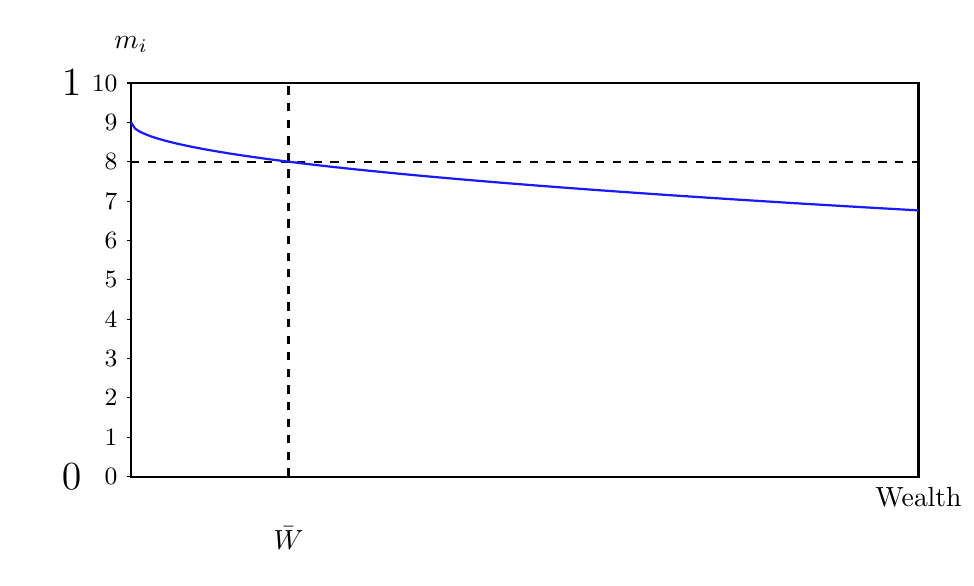
\begin{tikzpicture}[scale=.5]
% \def\bndmax{5}        %https://tex.stackexchange.com/questions/68462/filling-a-complex-region-with-tikz
% \def\bndmin{0.2}
\def\Y{10}  % height of y axis pecent
\def\W{20}  % length  of x axis
\def\Wbar{4}
\def\rbar{8}% this is the prime rate
% Equation   \[ r_i = (A + .5 \frac{\bar{W}}{W_i})\omega\]
% \def\Wmin{.63}  %This sets the lower limit fo the 
\def\Wmin{(\B*\Wbar)/(\Y/\rbar-\A)} %function to keep in in bounds
\tikzset{func/.style={thick,color=blue!90}}	
\draw [thick](\W,\Y)-- (0,\Y)node[left=.5cm]{\Large$1$}node[above=.25cm]{$m_i$} -- (0,0)node[left=.5cm]{\Large$0$}--(\W,0)node[below]{Wealth}--cycle;  	% Axes box
\draw [dashed, thick] (0,\rbar) -- (\W,\rbar);  	% Axes
\draw [thick,dashed] ( \Wbar,0)node[below=.5cm]{$\bar{W}$} -- (\Wbar,\Y);  	% Axes
\foreach \yi in {0,...,\Y} \draw (0,\yi)--(-.1,\yi)node[left]{\small$\yi$};
% \foreach \yi in {0,2,4,6,8,10} \draw (0,\yi)--(-.1,\yi));
% node[left]{\small$\yi$};
% \foreach \yi in {0,2,4,6,8,10}node at (-.1,yi) {{10*yi}} ;
\draw[func,domain=0:\W] plot [samples=200] (\x,(9-\x^.5/2);
\end{tikzpicture}
    \end{center}
    \caption{Individual borrowing ratio $m_i$ as a function of wealth}
    \label{fig-borrowing-ratio}
    \end{figure}


The borrowing ratio, $m$ is the fraction of a property's price that can be mortgaged. We assume that the bank uses a function of the form 


\begin{align}
m_i^{max\_permitted} =& \mathrm{max\_mortgage\_share} - 0.1*\left(\frac{\bar W}{ W_i}\right), \label{eqn-wealth-based-mortgage}  %^{\mathrm{wealth\_sensitivity}
\end{align} 
where $\bar{W}$ is mean wealth and $W_i$ is individual wealth.\footnote{To shift the curve  so that the curve approaches $m=0$ when $W=0$ we add  $Z=(1-m^{max})\bar W$ to the numerator and the denominator. The value is calculated by solving Equation~\ref{eqn-wealth-based-mortgage} for {$m_i^{max}=0$}.}


\subsubsection{Income-based mortgage maximum}
A common rule is that mortgage payments cannot exceed some fraction of income, $Y_i=\omega+ \psi + {r}S_i$, where $S_i$ is individual savings.
If $\mathbb{C}$ a person's carrying capacity, The annual payment that their income allows,  the capitalized value gives us an \textbf{income-based  mortgage maximum} of 


\begin{equation}
M^{max}_{Y,i} = \frac{\mathbb{C} (\omega+ \psi + {r}S_{Ni})}{r^{prime}},\label{eqn-income-based-mortgage}    
\end{equation}
% In addition, The Bank may have a maximum share of the price that it will lend, say $0.8P$. Because the actual price is unknown when buyers prequalify, this test limits the maximum bid computed below: \
% \[M^{max}i = min\left\{\frac{0.28*(\omega+w)}{r},  0.8P_0 \right\} \]
where ${r}$ is $i$'s rate of return on  $S_{Ni}=(S-M)$, the savings remaining after making the down payment,\footnote{If the constraint is binding we can  substitute $M^{max}$ for $M$and explicit function to get :
\begin{align}
M^{max}      &= 0.28 * (wage + r (S-M^{max})) / r'\nonumber\\
         &= 0.28 (wage + r (S)) / r' - 0.28 rM^{max}) / r'\nonumber\\
M^{max}(1+\frac{0.28 r}{r'}&=0.28 (wage + r S) / r'\nonumber\\
M^{max}   &=  \frac{0.28 (wage + r S )} {1+0.28 r}\nonumber   
\end{align}
} as the maximum a  buyer should pay. %\footnote{We  assume that the bank does not take transportation costs into account  when calculating income.}
%\footnote{If the expected return on a property is greater than the individual cost of borrowing, it would pay any agent to borrow as much as possible and purchase properties as they can available.}
In our model the bank uses a rule of this form to decide how much it is willing to lend to 

  \begin{figure}
    \centering
    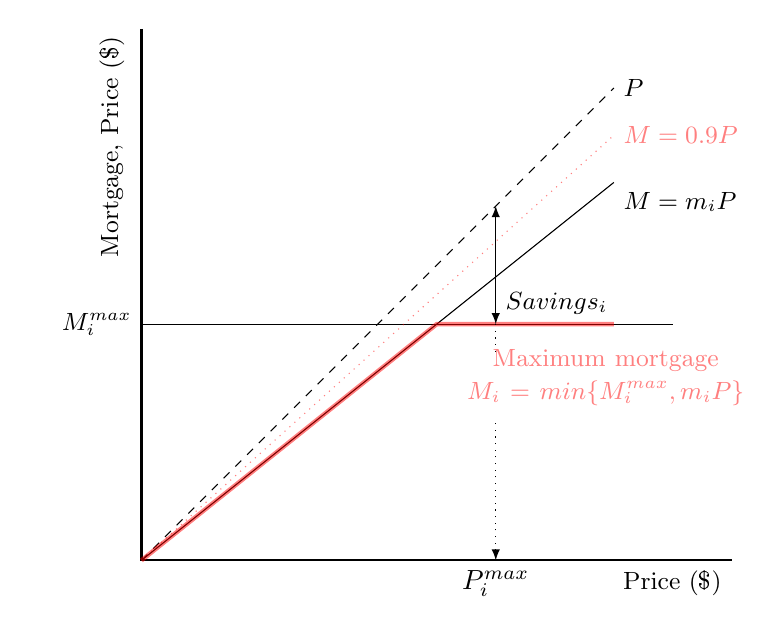
\begin{tikzpicture}	[scale=1.5]
%AXES
\draw[thick] (0,4.5) --(0,0)--(5,0)node[below left]{\small Price (\$)};
\node at (-.25, 3.5)[ rotate=90]{\small Mortgage, Price (\$)};
% M =Mi MAX
\draw[dashed] (0,0)--(4,4)node[right]{\small $P$};
\draw[] (0,2)node[left]{\small $M_i^{max}$}--(4.5,2);%node[right, red]{\small $M = M_i^{max}$};
% M =mi MAX
\draw[dotted,red, opacity=.5] (0,0)--(4,3.6)node[right]{\small $M = 0.9P$};
\draw[] (0,0)--(4,3.2)node[below right]{\small $M = m_iP$};
% COMBINED MAX RED
\draw[ultra thick, red, opacity=.5] (0,0)--(2.5,2)node[below right,  text width=4cm, align = center]{\small \\ Maximum mortgage \\ $M_i=min\{M_i^{max}, m_iP\}$}--(4.0,2);
% SAVINGS
\draw[latex-latex] (3,2)node[above right] {\small $Savings_i$}--(3,3);
% PMAX
\draw[dotted,latex- ] (3,0)node[below] {$P_i^{max}$}--(3,1.2);
\draw[dotted ] (3,2)--(3,1.72);
\end{tikzpicture}
    \caption{The bank's dual mortgage constraint and the savings constraint determine the maximum bid price.}
    \label{fig:dual-constraint}
    \end{figure}

\subsubsection{Combined mortgage maximum permitted by the bank for new buyers and second home buyers}

The above two equations specify two constraints on the mortgage.  Combining, we get 
\begin{align} 
M_i^{max} &= min \left\{ m_i^{max}*P, \ M^{max}_{Y,i} \right\}. 
\label{eqn-max-mortgage-combined}
\end{align}
The two constraints on mortgage size that the bank imposes are incorporated in the red line in Figure~\ref{fig:dual-constraint}. The maximum permitted mortgage is thus combined with the savings constraint to determine the maximum price that a potential home buyer can offer. The top dashed diagonal line, in Figure~{fig:dual-constraint}, is the price, $P =$ mortgage $+$ savings. The difference between the two diagonal lines is what the purchaser pays from savings. %\footnote{Equation~\ref{eqn-property-investment-return2} implies a `bang-bang' control---with all sales going to the richest participant unless there are limits on the size of capital flows. For our simulation, we implement such limits.} 
% \[M^{max}_{UY,i} = \frac{0.28*(\omega+ \psi)}{r}\] 
% It is the maximum the bank will let you pay.

% \subsection{The cost of capital}
% The cost of capital is known to differ for rich and poor. This model ties the individual cost of capital,  ${r}$ for agent $i$, to a prime rate, $\bar r$, and to individual wealth. Figure~\ref{fig-borrowing-cost} illustrates the cost of the borrowing model we implement, 
%  \[ {r} = (A + B \frac{\bar{W}}{W_i})\omega\]
% Where $\bar{W}$ is mean wealth and $W_i$ is individual wealth.   
% a kink because there are 2 constraints.  The actual mortgage must be below both lines.
% This is just the constraint. Up to the kink, little $m_i$ is a fraction of price. beyond at little $m_i$ becomes a different number - number based on little $m_i$ for everyone
% banks have an advantage since they can practically bid anything
% m - mortgage share
% P - realized price
% M - maximum - 
% \begin{figure}[!ht]
% \begin{center}
% 
% Large version
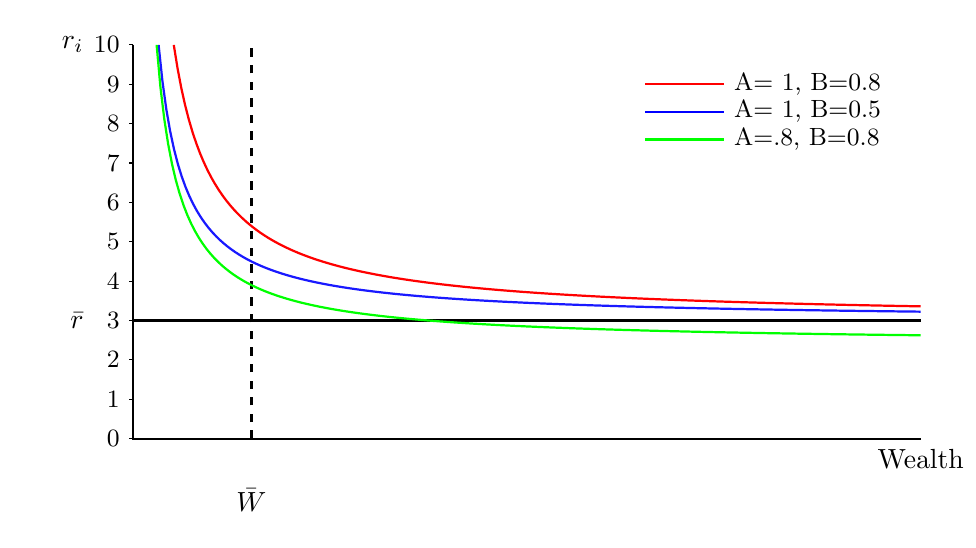
\begin{tikzpicture}[scale=.5]
%\def\bndmax{5}        %https://tex.stackexchange.com/questions/68462/filling-a-complex-region-with-tikz
%\def\bndmin{0.2}
\def \Y {10}  % height of y axis pecent
\def \W {20}  % length  of x axis
\def \Wbar {3} % jmeam wealth
\def \omega {3}
\def \A {1}  %was .5
\def \B {.5}
%Equation   \[ r_i = (A + .5 \frac{\bar{W}}{W_i})\omega\]
\def \Wmin{.63}  %This sets the lower limit fo the 
\def \Wmin{(\B*\Wbar)/(\Y/\omega-\A)} %function to keep in in bounds
	
\tikzset{func/.style={thick,color=blue!90}}	

\draw [thick] (0,\Y)node[left=.5cm]{$r_i$} -- (0,0)--(\W,0)node[below]{Wealth};  	% Axes
\draw [thick] (0,\omega)node[left=.5cm]{$\bar r$} -- (\W,\omega);  	% Axes
\draw [thick,dashed] ( \Wbar,0)node[below=.5cm]{$\bar{W}$} -- (\Wbar,\Y);  	% Axes

\foreach \yi in {0,...,\Y} \draw (0,\yi)--(-.1,\yi)node[left]{\small$\yi$};

\draw[func,domain=\Wmin:\W] plot [samples=200] (\x,{(\A+\B*\Wbar/\x)*\omega});
\def \A {.8}
\draw[func,domain=\Wmin:\W, green] plot [samples=200] (\x,{(\A+\B*\Wbar/\x)*\omega});

\def \A {1}
\def \B {.8}
\draw[func,domain=\Wmin:\W, red] plot [samples=200] (\x,{(\A+\B*\Wbar/\x)*\omega});

\draw [red,  thick](13, 9)--(15,9)node [right, black] {\small A=\ 1,\ B=0.8};
\draw [blue,  thick](13, 8.3)--(15,8.3)node [right, black] {\small A=\ 1,\ B=0.5};
\draw [green, thick](13, 7.6)--(15,7.6)node [right, black] {\small A=.8, B=0.8};
\end{tikzpicture}

% % Small version with equation and parameter values
% \[   r^h=\frac{ \delta(1+\dot p  - (1+r)m) \ + \rho   	-\kappa - t } {1-m}    \]
% \begin{tikzpicture}[scale=.35]
% %\def\bndmax{5}        %https://tex.stackexchange.com/questions/68462/filling-a-complex-region-with-tikz
% %\def\bndmin{0.2}
% \def \Y {10}  % height of y axis percent
% \def \W {18}  % length  of x axis
% \def \Wbar {3} % j mean wealth
% \def \omega {3}
% \def \A {1}  %was .5
% \def \B {.5}
% %Equation   \[ r_i = (A + .5 \frac{\bar{W}}{W_i})\omega\]
% \def \Wmin{.63}  %This sets the lower limit fo the 
% \def \Wmin{(\B*\Wbar)/(\Y/\omega-\A)} %function to keep in in bounds
	
% \tikzset{func/.style={thick,color=blue!90}}	

% \draw [thick] (0,\Y)node[left=.5cm]{$r_i$} -- (0,0)--(\W,0)node[below]{Wealth};  	% Axes
% \draw [thick] (0,\omega)node[left=.5cm]{$\bar r$} -- (\W,\omega);  	% Axes
% \draw [thick,dashed] ( \Wbar,0)node[below=.5cm]{$\bar{W}$} -- (\Wbar,\Y);  	% Axes

% \foreach \yi in {0,...,\Y} \draw (0,\yi)--(-.1,\yi)node[left]{\tiny$\yi$};

% \draw[func,domain=\Wmin:\W] plot [samples=200] (\x,{(\A+\B*\Wbar/\x)*\omega});
% \def \A {.8}
% \draw[func,domain=\Wmin:\W, green] plot [samples=200] (\x,{(\A+\B*\Wbar/\x)*\omega});

% \def \A {1}
% \def \B {.8}
% \draw[func,domain=\Wmin:\W, red] plot [samples=200] (\x,{(\A+\B*\Wbar/\x)*\omega});

% \draw [red,  thick](10, 9)--(12,9)node [right, black] {\tiny A=\ 1,\ B=0.8};
% \draw [blue,  thick](10, 8)--(12,8)node [right, black] {\tiny A=\ 1,\ B=0.5};
% \draw [green, thick](10, 7)--(12,7)node [right, black] {\tiny A=.8, B=0.8};

% \def \W {19}  % length  of x axis
% \node[right] at (\W,9.5){\small$\delta=$discount factor};
% \node[right] at (\W,8.5){\small$\dot p=$appreciation rate};
% \node[right] at (\W,7.5){\small$r=$borrowing rate};
% \node[right] at (\W,6.5){\small$m=$mortgage/price};
% \node[right] at (\W,5.5){\small$\rho=$rental  rate};
% \node[right] at (\W,4.5){\small$\kappa=$op cost rate};
% \node[right] at (\W,3.5){\small$t=$tax rate};
% \node[right] at (\W,2.5){\small$\upsilon=$use value rate};
%  \end{tikzpicture}



% One blue line with x-shift, y-shift
% \begin{figure}
% \begin{tikzpicture}[scale=.5]
% %\def\bndmax{5}        %https://tex.stackexchange.com/questions/68462/filling-a-complex-region-with-tikz
% %\def\bndmin{0.2}
% \def \Y {10}  % height of y axis pecent
% \def \W {20}  % length  of x axis
% \def \Wbar {3} % meam wealth
% \def \rbar {3}% this is the prime rate 

% %\def \Wmin{(\B*\Wbar)/(\Y/\rbar-\A)} %function to keep in in bounds
% \tikzset{func/.style={thick}}	
% 	% Axes
% \draw [thick] (0,\Y)node[left=.5cm]{$r_i$} -- (0,0)--(\W,0)node[below]{Wealth};  
% \foreach \yi in {0,...,\Y} \draw (0,\yi)--(-.1,\yi)node[left]{\small$\yi$};
% \draw [thick] (0,\rbar)node[left=.5cm]{$\bar r$} -- (\W,\rbar);  	% Axes
% \draw [thick,dashed] ( \Wbar,0)node[below=.5cm]{$\bar{W}$} -- (\Wbar,\Y);  	% 

% \def \A {1} %vertical shift aroung \rbar, the prime rate
%  \def \B {1}  % Scales the exponential curveBLUE
%  \def \C {1}  %right shift  
% % \def \Wmin {.4+\B}  %This sets the lower limit fo the 
% \def \Wmin {(\B*\Wbar)/(\Y-\rbar+\A) +\C} %function to keep in in bounds

% \draw[func,domain=\Wmin:\W, color=blue!90] plot [samples=200] (\x,{\rbar-\A+\B*\Wbar/(\x-\C))});
% \node  [align=left, text width =2cm ] at (13, 8.3) {\small y-shift=\A \newline scale=\B \newline x-shift= \C};

%  \end{tikzpicture}
% \caption{Individual borrowing cost as a function of wealth II}
% \label{fig-borrowingrate2}
% \end{figure}

% The rates $\delta,\ \sigma,$ and $r$ depend on the period, $T$. 


% LARGE WITH DIFFERENT PARAMETER VALUES THAN MAOIN FIGURE - MORE SPREAD

% \begin{figure}
% \begin{tikzpicture}[scale=.5]
% %\def\bndmax{5} % https://tex.stackexchange.com/questions/68462/filling-a-complex-region-with-tikz
% %\def\bndmin{0.2}
% \def \Y {10}    % height of y axis as a pecent
% \def \W {20}    % length  of x axis
% \def \Wbar {3}  % mean wealth
% \def \rbar {3}  % the prime rate 

% % Equation   \[ r_i = (A + .5 \frac{\bar{W}}{W_i})\omega\]
% \def \Wmin{.63}  %This sets the lower limit fo the 
% \def \Wmin{(\B*\Wbar)/(\Y/\rbar-\A)} %function to keep in in bounds
% \tikzset{func/.style={thick}}	

% % Axes
% \draw [thick] (0,\Y)node[left=.5cm]{$r_i$} -- (0,0)--(\W,0)node[below]{Wealth};  
% \foreach \yi in {0,...,\Y} \draw (0,\yi)--(-.1,\yi)node[left]{\small$\yi$};
% \draw [thick] (0,\rbar)node[left=.5cm]{$\bar r$} -- (\W,\rbar);  	% Axes
% \draw [thick,dashed] ( \Wbar,0)node[below=.5cm]{$\bar{W}$} -- (\Wbar,\Y);  	% 

% \def \A {1.0}  \def \B {0.5} %BLUE
% \draw[func,domain=\Wmin:\W, color=blue!90] plot [samples=200] (\x,{(\A+\B*\Wbar/\x)*\rbar});
% \draw [ultra thick, color=blue!70 ](13, 8.3)--(15,8.3)node [right, black] {\small A=\A,\ B=\B};

% \def \A {0.5} 
% \def \B {0.5} % GREEN
% \draw[func,domain=\Wmin:\W, color=green] plot [samples=200] (\x,{(\A+\B*\Wbar/\x)*\rbar});
% \draw [thick,  color=green](13, 7.6)--(15,7.6)node [right, black] {\small A=\A, B=\B};

% \def \A {1.0}  \def \B {0.8} % RED
% \draw[func,domain=\Wmin:\W, red] plot [samples=200] (\x,{(\A+\B*\Wbar/\x)*\rbar});
% \draw [thick,  color=red](13, 9)--(15,9)node [right, black] {\small A=\A,\ B=\B};
% % KEY
% \end{tikzpicture}
% \caption{Individual borrowing cost as a function of wealth}
% \label{fig-borrowingrate1}
% \end{figure}
% Figure of cost of borrowing
% \caption[Borrowing cost for agents depending on wealth.]{Borrowing cost for agents depending on wealth, with different values for parameters $A$ and $B$ in Equation~\ref{eqn-interest-wealth-relationship}.} %$A=1$  $B=0.5$ (blue);  $A=1$  $B=0.8$ (red), and  $A=.8$  $B=0.8$ (green).}
% \label{fig-capital-cost}
% \end{center}
% \end{figure}

\subsubsection{Individualized borrowing rates} \label{sec:borowing-rate}

    \begin{figure}
    \centering
    
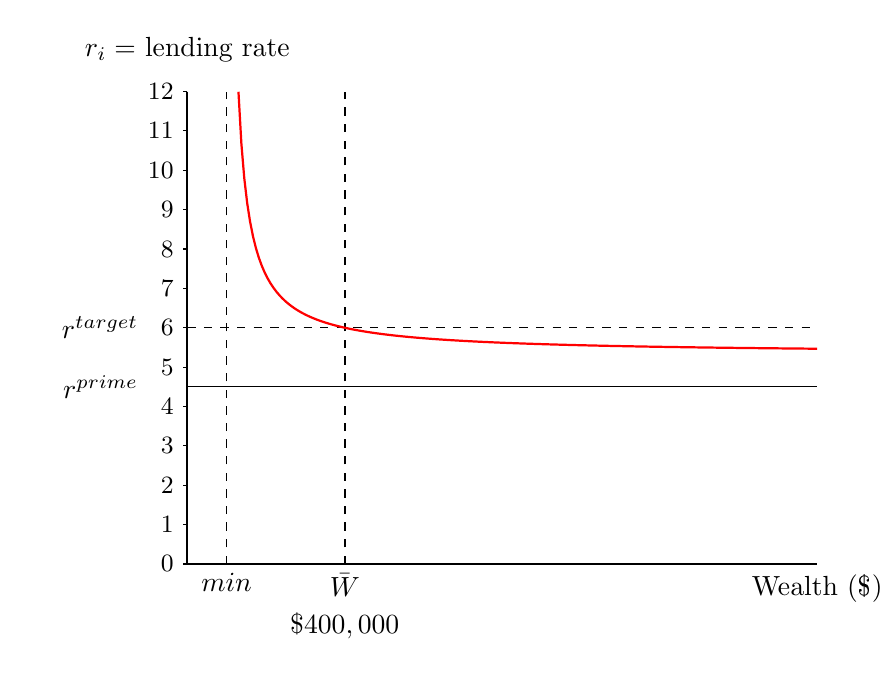
\begin{tikzpicture}[scale=.5].  %  Individual borrowing rate r\_i
%\def\bndmax{5}        %https://tex.stackexchange.com/questions/68462/filling-a-complex-region-with-tikz
%\def\bndmin{0.2}

\def \k {2}    % budget for rectangular hyperbola
\def \Wbar {4} % meam wealth in hundred thousands
\def \Wmin {1} % This sets the lower limit for lending in hundred thousands
\def \W {16}    % length  of x axis
\def \rbar {4.5} % N.B.:  this is r bar
\def \Y {12}     % height of y axis percent
\def \margin {1.5}
\def \target {\margin+\rbar} % target interest rate for bank
\def\bndmin {0.3} % This limits the function on the right so that it stays in the plotting frame
%\def \Wmin{(\B*\Wbar)/(\Y/\rbar-\A)} %function to keep in in bounds. NEEDS WORK
	
\tikzset{func/.style={thick}}	
\draw [thick] (0,\Y)node[above=.25cm]{$r_i=$ lending rate} -- (0,0)--(\W,0)node[below]{Wealth (\$)}node[below=.5cm] {};   	% Axes

\draw [thin] (0,\rbar) node[left=.5cm]{$r^{prime}$} -- (\W, \rbar);  	% % bank rate line
\draw [thin, dashed] (0,\target) node[left=.5cm]{$r^{target}$} -- (\W, \target);  	% % target rate line
\node at ( \Wbar, 0)[below=.5cm]{$\$400,000$};  
\foreach \yi in {0,...,\Y} \draw (0,\yi)--(-.1,\yi)node[left]{\small$\yi$};  %$ put the scale on the y axis

\draw [thick, dashed] (\Wbar, 0)node[below] {$\bar{W}$} --  (\Wbar, \Y);  	%. Wbar
\draw [thin, dashed]  (\Wmin, 0)node[below] {$min$} -- (\Wmin, \Y);  %minimum lending wealth

\draw[func,domain={\W-\Wmin}:\bndmin, red] plot [samples=200] (\x+\Wmin,{\target+\k/\x - \k/(\Wbar-\Wmin)});

\end{tikzpicture}


% \begin{tikzpicture}[scale=.5]
% %\def\bndmax{5}        %https://tex.stackexchange.com/questions/68462/filling-a-complex-region-with-tikz
% %\def\bndmin{0.2}
% \def \Y {10}  % height of y axis pecent
% \def \W {20}  % length  of x axis
% \def \Wbar {4} % jmeam wealth
% \def \omega {3} % N.B.:  this is r bar

% %Equation   \[ r_i = (A + .5 \frac{\bar{W}}{W_i})\omega\]
% \def \Wmin{.63}  %This sets the lower limit fo the 
% \def \Wmin{(\B*\Wbar)/(\Y/\omega-\A)} %function to keep in in bounds
	
% \tikzset{func/.style={thick}}	

% \draw [thick] (0,\Y)node[left=.5cm]{$r_i$} -- (0,0)--(\W,0)node[below]{Wealth};  	% Axes
% \draw [thick] (0,\omega)node[left=.5cm]{$\bar r$} -- (\W,\omega);  	% Axes
% \draw [thick,dashed] ( \Wbar,0)node[below=.5cm]{$\bar{W}$} -- (\Wbar,\Y);  	% Axes

% \foreach \yi in {0,...,\Y} \draw (0,\yi)--(-.1,\yi)node[left]{\small$\yi$};

% %     ORANGE
% % \def \A {1} \def \B {.8}
% % \draw[func,domain=\Wmin:\W, orange] plot [samples=200] (\x,{(\A/\x+\B*\X/\Wbar/\x)*\omega});
% % \def \A {1} \def \B {.1}
% % \draw[func,domain=\Wmin:\W, orange, dashed] plot [samples=200] (\x,{(\A+\B*\X/\Wbar/\x)*\omega});

% %     RED
% \def \A {1} \def \B {.8}
% \draw[func,domain=\Wmin:\W, red] plot [samples=200] (\x,{(\A+\B*\Wbar/\x)*\omega});
% \def \A {1} \def \B {.1}
% \draw[func,domain=\Wmin:\W, red, dashed] plot [samples=200] (\x,{(\A+\B*\Wbar/\x)*\omega});

% %.    BLUE
% \def \A {1} \def \B {.5}
% \draw[func,domain=\Wmin:\W, blue!90] plot [samples=200] (\x,{(\A+\B*\Wbar/\x)*\omega});
% %     GREEN
% \def \A {.8} \def \B {.8}
% \draw[func,domain=\Wmin:\W, green] plot [samples=200] (\x,{(\A+\B*\Wbar/\x)*\omega});
% %.    BLACK
% \def \A {.5} \def \B {.5}
% \draw[func,domain=\Wmin:\W, black] plot [samples=200] (\x,{(\A+\B*\Wbar/\x)*\omega});


% \draw [red,  thick](13, 9)--(15,9)node [right, black] {\small A=\ 1,\ B=0.8};
% \draw [red,  thick, dashed](13, 9.7)--(15,9.7)node [right, black] {\small A=\ 1,\ B=0.1};
% \draw [blue,  thick](13, 8.3)--(15,8.3)node [right, black] {\small A=\ 1,\ B=0.5};
% \draw [green, thick](13, 7.6)--(15,7.6)node [right, black] {\small A=.8, B=0.8};
% \draw [black, thick](13, 6.9)--(15,6.9)node [right, black] {\small A=.5, B=0.5};
% \end{tikzpicture}


\label{fig-capital-cost}
    \caption{Individual borrowing rate $r_i$ price of capital}
    \label{fig:Wealth-based}
    \end{figure}

The cost of capital differs for rich and poor. We tie the individual cost of capital %,  ${r}$, for agent $i$ 
to the lender's target rate $r^{target}$, and to individual wealth. Figure~\ref{fig-capital-cost} illustrates the cost of the borrowing model we implement, which is roughly consistent with the stylized facts about lenders. 
\begin{equation}
{r} = r^{target}+ K/(W-W_{min}) -K/(\bar W - W_{min})\label{eqn-interest-wealth-relationship}
\end{equation}
for $W>W_{min}$, where  $r^{target}$ is the bank's target rate of return,  $\bar{W}$ is mean wealth and $W_i$ is individual wealth, $W_{min}$ is the level of wealth the bank requires to lend at all, and $K$ is a parameter for the wealth-sensitivity of lending. The denominator in the last two terms is simply wealth above the lender's minimum. We assume that the wealthy are lower-risk borrowers and are given preference on rates. The final term ensures that the target rate is charged for borrowers with average wealth.


%The individual cost of capital,  ${r}$ for agent $i$ is tied to a prime rate, $\bar r$ or the bank's target rate, $r^{target}$, and and varies with individual wealth. %Figures~\ref{fig-borrowing-rate1} % and ref{fig-borrowing-rate1} 
%illustrates a  possible  cost-of-borrowing models 

% \begin{align}
%  {r} =  &  \left(A + B \frac{\bar{W}}{W_i}\right) \bar r       \label{eqn-incomeandr1}  \\
%  {r} =  &  \left(\bar r - A + B *\frac{\bar W}{W_i - C}\right) \label{eqn-incomeandr2}  \\
% \end{align}
% Where $\Bar{W}$ is mean wealth and $W_i$ is individual wealth. In Equation~\ref{eqn-incomeandr2},  A determines y-shift, B, the scale, and C the  x-shift for the curve.


\subsubsection{Declining principle}\label{sec:declining-principle}

Mortgages are renewed after $\mathbb{T}$ years. During that period some of the principle has been paid off. This is most important when a property is sold. The seller gets $P-M_{i,\mathbb{T}}$, where  $M_{i,\mathbb{T}}$ is its remaining mortgage.

% % {\color{red} 

% **** ADD BACK
% \textbf{Footnote on size of mortgage at renewal.}
% % \footnote{We would need to calculate the decline balance when  renewal came up to know what assets a person has. We need a function that gives us the size of the mortgage remaining at each renewal or at the time of sale, $M_{i,term}$, for each subsequent renewal. The  function depends on the mortgage renewal term, $\mathbb $, the number of terms $term$  that have passed since the purchase, the interest rate ${r}$ and the payment. Mortgages are usually intended to be paid off over, say,  $L=25$ years If we use $T=5$, there will be 4 renewals and the house will b =e paid off at the end of the fifth. Payments are larger than the interest, so the amount owed at the end of each month declines. At the end of month N it is

% % There is a standard formula for choosing the payment so that the mortgage it is paid off at the end of the mortgage life, $L$. Say $n$ is the number of monthly payments (for example 25*12=300) %https://en.wikipedia.org/wiki/Mortgage_calculator

% % \[payment= {r}^\mathbb{\mathbb{T}}M \left[\frac{(1+{r}^\mathbb{T}\mathbb{T})^n}{(1+{r}^\mathbb{T})^n-1} \right]\]
% % Where ${r}^\mathbb{T}$ is the interest rate compounded for $\mathbb{T}$ periods.
% % % \begin{align}
% % % M_{N*T}&=(1+r)^{N}M_0-p_{N}c\nonumber \\
% % % &{}=(1+r)^{N}P-{\frac {(1+r)^{N}-1}{(1+r)-1}}c \nonumber\\
% % % &{}=(1+r)^{N}P-{\frac {(1+r)^{N}-1}{r}}c
% % % \end{align}
% % % Amount owed at end of month N}
% % %}
% % }
% % }

% \textbf{We can assume is paid off the mortgage when we discuss retirement decisions. If as person works 40 years and buys a house by the 15th year they will have paid off their  mortgage and collect the entire price if they sell. }  

% When else will we need to consider this problem? If we let people buy a revenue property - then wealth includes $P-M$. Also if we let people die early, or allow them to change homes part way through a career- for family reasons.


\subsection{Bid price}\label{sec:bid-price}
A bidding process determines the realized market price, with bidders taking into account potential capital gains. In this section, we describe the formation of the maximum bid price that we use in the bidding model. The maximum \gls{bid price}, $P_{B,ij}^{max}$ %, where i and j refer to the individual and the property involved,\footnote{We suppress the $ij$ identifiers for the rest of this chapter. }  
is the value of a property to the owner or to a potential buyer. It will differ across individuals depending on their cost of capital, discount rates,  savings, and access to mortgage funding. The same equation used to calculate the bid price used to compute the \gls{reservation price}, the minimum price that an owner will sell a property for. 

The model distinguishes between two types of investment buyers, institutional buyers and homeowners buying an investment home. They use the same investment formula, but may have different values of the parameters determining their bid prices.

We first calculate the net present value of the purchase, then divide by the amount of capital employed, which we assume is simply the size of the down payment made at the beginning of the period. This gives us a rate of return.\footnote{An alternative approach would be to calculate an \gls{internal rate of return} (IRR), but the IRR is in general the solution to a polynomial and does not guarantee a single-valued result \cite{robinsonOptimalTerminationIRR1996}. Multiple real-valued  IRRs may arise;  complex-valued IRRs may arise;  the IRR is, in general, incompatible with the \gls{net present value} (NPV) in accept/reject decisions; the IRR ranking is, in general, different from the NPV ranking; the IRR criterion is not applicable with variable costs of capital. Ways to salvage the IRR as a usable criterion have been proposed that are consistent with our approach \cite{magniAverageInternalRate2010}.} The rate of return on the investment must exceed some required rate of return. This condition allows us to calculate the maximum bid that will satisfy that criterion.}
% We assume that agent may be  speculating on potential \glspl{capital gain} as well as on the \gls{use value} or net market rent they get from the property. We therefore treat the purchase as an investment decision and compute a rate of return, $v$, conditional on the price paid. This allows us to 
We then solve this for the maximum bid, $P_{max}^{bid}$ that achieves the desired rate of return. 


% The underlying value of a home is the capitalized value of the services it provides, which are perpetual.  Rents, however, depend on urban productivity and may change over time. Any expected increase in future rents capitalized into the market price of a home as a capital gain for the owner. Home prices should respond to expectations.

% As Horowitz \cite{horowitzBiddingModelsHousing1986} notes, a prospective buyer considering a vector of attributes of the property, including the seller's asking price and the property taxes, transaction costs, and financing costs at a specified price. The  potential buyer also is likely to have estimates of the maintenance costs and resale value of the house, although these may be highly subjective. All of these factors shape whether an investment is profitable. To make a comparison with alternative investments, it is necessary to compute a rate of return.

The agent who purchases makes a down payment, $D$ on a house for a price, $P_0$, and agrees to pay off a mortgage, $M$ with interest at the end of the mortgage period.  The purchaser  receives the increased price 
$P_T = (1 + \dot P)^\mathbb{T}P_0 =(1+\dot P_\mathbb{T})P_0 $, 
after a period $\mathbb{T}$, Where $\dot P$  is the expected annual rate of price increase and we define $\dot P^\mathbb{T}$
or $\dot P^{^\mathbb{T}}$ 
as the $\mathbb{T}$-period  price-growth rate. The agent also receives either the net market rental value of the property throughout the period, $\mathcal{R}_N$, or if the owner is also the resident, the locational rents. 
 
% With a price-growth rate of $\dot P$ per year, the growth over $T$ years is $(1+\dot P)^\mathbb{T}$, and  %and a 5 year mortgage period, 
% the expected price at the end of the period is:

% \[P_M^{Te}=P_0(1+\dot P)^\mathbb{T}\]

% If, for example price growth is 10\%, $\dot P= 0.1$, the {capital gain}, or growth, over a 5-year mortgage term is 0.61051 $\approx$ 60\% of the original price, $P_0$.

%The expected rate of price growth, $P_{M_j}^\epsilon$, is an estimate based on rents and past market behaviour. In our computational model we employ a regression model to generate an \gls{expected market price} based on past prices. The rate of price growth $\dot P$ we use in our model of investor behaviour is derived from the same regression model.




% TODO SOME REFERENCES - what are these? MOVE? \cite{anselinModernSpatialEconometrics2014, gelmanDataAnalysisUsing2006}.


 
\subsubsection{Rent and mortgage costs}
Both mortgage payments and net rent revenue can be calculated as sum of regular payments, each of which accumulates interest to the end of the mortgage period. This is called a ``uniform series compound amount.'' \cite{sullivanEngineeringEconomy2003} For net rent at the end of the mortgage renewal term we write
\begin{equation}
\mathcal{R}_{N, \mathbb{T}}= \frac{(1+r)\mathbb{^\mathbb{T}}-1}{r}\mathcal{R}_N.     
\end{equation}

The regular mortgage payment for each period is $rM=rmP_0$.\footnote{We assume that the regular payment covers only the interest and that the full mortgage is due at the end of the period.} Using the same calculation, the value of the mortgage payments is 
\begin{equation}
\mathcal{M}_{\mathbb{T}} = \frac{(1+r)^\mathbb{T}-1}{r}rmP_0. 
\end{equation}
Both these amounts are discounted by $\delta^\mathbb{T}$ to the present. % in our calculation.
 
\subsection{The value of an investment with price growth or interest}
 The model in this section is central to our agents' housing purchase decisions. It incorporates individual access to capital and capital costs, expected capital gains and property revenues.  
 
 For an agent, the value $V$ of a property investment over  $\mathbb{T}$ years is the capital gain, $P_{^\mathbb{T}}-P_{0}$, minus financing costs, plus net rent. % revenues.
% \[\mathcal{R}_{N, \mathbb{T}}=  \delta^\mathbb{T}\frac{(1+r)^\mathbb{T}-1}{r}\mathcal{R}_N  \]
% To keep the notation simple, let 
% \[\delta_r^\mathbb{T}=\delta^\mathbb{T}\frac{(1+r)^\mathbb{T}-1}{r}\]
% The present value of the mortgage repayment plus the accumulated interest be 
% \[\bar M^\mathbb{T}_r = \delta^\mathbb{T}\frac{(1+r)^\mathbb{T}-1}{r}\]
 We can write $V$ in terms of the purchase price, and several individual parameters: interest rate, share of the price that can be mortgaged and discount rate %\footnote{The down payment could be deducted in advance, but if the discount rate is equal to the interest rate it drops out completely.}
 
 \begin{align}
V &= \delta^\mathbb{T}\left( P_\mathbb{T}-P_0-\mathcal{M}_{\mathbb{T}}- M+ \mathcal{R}_{N, \mathbb{T}} \right)      \nonumber\\
&= \delta^\mathbb{T}\left( P_\mathbb{T}-P_0- \left(\frac{(1+r)^\mathbb{T}-1}{r}rmP_0\right)- M+ \mathcal{R}_{N, \mathbb{T}} \right)      \nonumber\\
&= \delta^\mathbb{T} \left(
\dot P_\mathbb{T} P_0 -\left((1+r)^\mathbb{T}-1\right)mP_0-mP_0
 +  \mathcal{R}_{N, \mathbb{T}} \right) 
%\label{first_sub}\nonumber
\\
  &= \delta^\mathbb{T} \left((\dot P_\mathbb{T} - (1+r)^\mathbb{T}m) P_0 + \mathcal{R}_{N, \mathbb{T}}\right),\label{eqn_investment_value}
\end{align}
where $\dot P_\mathbb{T}=\frac{P_\mathbb{T}-P_0 }{P_0}$  is the expected  change in the market price over the term of the mortgage as a fraction of the original price.
$V$ is the net present value of buying and selling after one mortgage renewal period of $\mathbb{T}$ years. %All rates are scaled to the length of the period to avoid the need for compounding calculations. 
% The function has four individualized parameters, $\delta$, $\dot p$, $r$, $m$. %, as well as any factors that affect the rent or other terms.


\subsubsection{Rate of return on investment}
We divide $V$ by the size of the down payment, $D=P_0-mP0$, to get the  rate of return  

\begin{align}
r^{return} =
  &= \frac{V}{D}  \nonumber \\
  &= \delta^\mathbb{T} \left((\dot P_\mathbb{T} - (1+r)^\mathbb{T})m \frac{P_0}{D} + \frac{\mathcal{R}_{N, \mathbb{T}}}{D}\right) \nonumber \\
%  &= \delta^\mathbb{T} \left((\dot P_\mathbb{T} - (1+r)^\mathbb{T})m \frac{P_0}{P_0-mP_0} + \frac{\delta_r^\mathbb{T}\mathcal{R}_{N, \mathbb{T}}}{P_0-mP_0}\right)\\
   &= \delta^\mathbb{T} \left((\dot P_\mathbb{T} - (1+r)^\mathbb{T})m \frac{P_0}{P_0-mP_0} + \frac{\mathcal{R}_{N, \mathbb{T}}}{P_0-mP_0}\right) \nonumber \\
  &= \frac{\delta^\mathbb{T}}{1-m} \left((\dot P_\mathbb{T} - (1+r)^\mathbb{T})m  + \frac{\mathcal{R}_{N, \mathbb{T}}}{P_0}\right).\label{eqn-property-investment-return1} 
\end{align}
Notice that the return depends on the price paid, $P_0$, which is determined in the market though competitive bidding.

\subsubsection{Capital gains tax}
The \gls{capital gains tax} is %one of the most interesting policy parameters to consider. It is 
a tax on the increase in value of a property that results form an increase in the price. The capital gains tax is a tax on speculative return on housing as an investment. In our model captures some or all of the expected gain from rising locational rents. We can introduce it in Equation~\ref{eqn-property-investment-return1} by multiplying $\dot P_\mathbb{T}$ by 1 minus the capital gains tax rate, representing the share of the capital gains that a buyer is permitted to keep. We allow the rate for occupant owners to differ from the rate for non-occupant owners.


\subsection{Criterion for investment}
Equation~\ref{eqn-property-investment-return1} provides a criterion for investors. %\footnote{Section~\ref{sec-extensions-conversion}, in Appendix~\ref{appendix-future-work}, discusses the potential for more detailed modelling of the land assembly and development process.} 
 Agents invest if  their expected return is greater than the target return they are seeking:
\begin{equation}
r^{target}\le r^{return} 
\label{eqn-property-investment-return2}
\end{equation}
For the bank R target is the prime rate plus a margin. For individuals it woulds be the the best alternative investment they have. It can be argued that  $r^{target}_i$ should be the long-term bond rate. We provisionally set $r^{target}_i=r^{prime}$.

\subsubsection{Maximum bid for investors}
Equation~\ref{eqn-property-investment-return2} combined with the rate of return calculation in Equation~\ref{eqn-property-investment-return1} are used to calculate a maximum bid price for investors for use in the bargaining model.
% Equation~\ref{eqn-return-on-investment} makes it clear that the estimated rate of return depends on subjective magnitudes,$\delta$ and $\dot P_M^e$, attributes of the property, $ \mathcal{R}_N$, and  individual financial position, $r$, $m$.
% 
%Buyers will not initially bid the maximum and sellers will generally set an asking price $P^{ask}$ higher than their reservation price $P_R$, so we build a simple bargaining process.
Buyers and sellers calculate the maximum amount they are willing to pay for a property.  Investors are not concerned with amenities, while residents are. %Since investors are concerned with the rent they can collect, however
Amenities enter through the net rent term for investors, to the extent that residents are willing to pay for amenity. Buyers differ in having individualized values for $r$, $\delta$, $m$, and $M$.%To simplify notation, we continue to omit  $i$ subscripts for each of these terms
\footnote{Transaction costs on the sale are omitted. They are actually large. We can easily add a term to  Equation~\ref{eqn:maximum-bid} to examine the effect of transaction costs.} % on the distribution of wealth.}

\begin{align}
r^{target}& \le \frac{\delta^\mathbb{T}}{1-m} \left((\dot P_\mathbb{T} - (1+r)^\mathbb{T})m  + \frac{\mathcal{R}_{N, \mathbb{T}}}{P_B^{max}}\right)\nonumber\\
\frac{(1-m)}{\delta^\mathbb{T}}r^{target} &\le \dot P_\mathbb{T} - (1+r)^\mathbb{T}m  +   \frac{\mathcal{R}_{N, \mathbb{T}}}{P_B^{max}} \nonumber\\
\frac{(1-m)r^{target}}{\delta^\mathbb{T}} - \dot P_\mathbb{T} + (1+r)^\mathbb{T}m &\le  \frac{\mathcal{R}_{N, \mathbb{T}}}{P_B^{max}}\nonumber\\
P_B^{max} &\le  \frac{\mathcal{R}_{N, \mathbb{T}}}{(1-m)r^{target}/\delta^\mathbb{T} - \dot P_\mathbb{T} + (1+r)^\mathbb{T}m}. \label{eqn:maximum-bid}
\end{align}
We call this  $i's$ maximum bid.\footnote{The denominator in Equation~\ref{eqn:maximum-bid} can be seen as an adjusted rate of return for capitalizing net rents, analogous to the value of $r$ in the standard capitalization formula.} 
It represents the maximum a buyer is willing to pay, the value of the stream of rent plus any capital gains. % It is also the most reasonable reservation price.%\footnote{In principle Equation~\ref{eqn:maximum-bid} could be calculated for all potential buyers and sellers for every property. In practice, only a subset of potential buyers and sellers are in the market at any time.} 
If the buyer intends to become a resident, the net rent term Equation~\ref{eqn:maximum-bid} is replaced by a housing-services-and-amenity term, which represents non-monetary income. % and is another form of locational rent. 

\subsubsection{A simple proxy for $\dot P_\mathbb{T}$}

The \gls{market price} or the price at which a property is exchanged on the market, $P_M$ will not be known in advance, nor will the future sale price.  In order to make decisions, agent $i$ must form an \glspl{expectation} or prediction $P_{M_i}^{\epsilon}$ of the as yet unrealized future market price. Case and Shiller observe that, ``People seem to form their expectations from past price movements rather than having any knowledge of fundamentals. \cite{caseThereBubbleHousing2003}. They further argue that the 1-year expectations are fairly well described as attenuated versions of lagged actual 1-year price changes. Our $\dot P_\mathbb{T}$ is a forecast or expectation by agents in the model of the change in price over a period $\mathbb{T}$.

Since our version of the \gls{Alonzo model} implies that house prices will rise by the capitalized value of an increase in the wage premium, a rational investor might use a forecast of the wage premium to develop a long-term forecast of house prices, and from that of $\dot P_\mathbb{T}$. %The specific value to use for $\die{\omega}{t}$ might depend on assumptions agents make about adjustment,  the variability of $P$, and the observability of $\omega$, but 
We will assume that agents simply observe the the most recent change in $\omega$  correctly and expect it to persist.\footnote{In principle, agents might form an expectation by observing past prices for each class of home. To mimic this process we could compute average price changes per period at each distance from the centre and use them to form a forecast for the mortgage period $\mathbb{T}$. }

In Equation~\ref{eqn_investment_value} we defined $\dot P$ as $\frac{P_\mathbb{T}-P_0}{P_0} $, where $\mathbb{T}$ indicates the. end of the mortgage period. $P_0$ is the warranted price, 
\[P_W =\frac{1}{r}\left[\omega - {dc} + \mathbb{A} + a\psi\nonumber  + a*b*\psi\right]\]
Only the wage premium changes in this analysis. A change in the wage premium that is expected to be permanent results in a change in the warranted price:  \[\die{P_W}{t} = \frac{1}{r}\die{\omega_t}{t}.\]
If we assume that the price will continue to change at the same rate over the mortgage term, the change is compounded, and we write

%P_W &=\frac{1}{r}\left[\omega - {dc} + \mathbb{A} + a\psi\nonumber  + a*b*\psi\right] \nonumber\\

%Only $\omega$ is expected to change over time, so  
%Since \[\dot P= \frac{\die{P_W}{t}}{P_T} \]


\begin{align}
\dot P  &= \frac{1}{r}\left[\left(\frac{\omega_t-\omega_0}{\omega_0}+1 \right)^\mathbb{T}-1\right], \nonumber\\
        &=\frac{1}{r}\left[\left(\frac{\omega_t}{\omega_0} \right)^\mathbb{T}-1\right]. \nonumber
\end{align}



\subsection{Illustrating constraints on the bid price} \label{sec:bids-and-reservation}
 
Buyers calculate their maximum bid based on value, but actual bids are constrained by the mortgage limits imposed by the bank illustrated in Figure~\ref{fig:dual-constraint} and the buyer's savings. The mortgage constraint may or may not bind, depending on the price of the final price. Figure~\ref{fig:savings-constraint} illustrates how these considerations affect the actual bid. 

We choose a price on the horizontal axis and project it up to the black dashed diagonal. Three lines show the levels of the constraints at that price.
% {\color{red}
%Purchasers may be financially constrained by the combination of mortgage availability and savings, as illustrated in Figure~\ref{fig:savings-constraint}. 
\begin{enumerate}
    \item The horizontal dashed line $P_B^{max}$ represents \textbf{the maximum the buyer is willing to pay}, as calculated in Equation~\ref{eqn:maximum-bid}, if the mortgage funding were available. No bid will be above this line. 

    \item The kinked thick red line combines the three conditions on the size of the mortgage imposed by the bank based on wealth and income and on the bank's equity requirement.
   
    \item The thick blue line, $min\left\{m_i P,\  M_{i}^{max}\right\}+ S $, represents the purchaser's combined financial constraints, determined by mortgage availability and savings. It is \textbf{the maximum the buyer is able to pay}.  No bid will be above this line either.
\end{enumerate}
 As a result the combined curve will be the constraint for buyers, and the requirement that the bid be below both the blue and black lines can be written

\begin{equation}
    Constrained\; P_{B} \le min \left\{P^{max}_B, min\left\{m_i P,\  M_{i}^{max}\right\}+ S \right\}.  \label{eqn:bid_diagonal}
\end{equation}

% \begin{align}
%     constrained\; P_B^{max} &\le min\left\{ P_B^{max} ,  \frac{M^{max}}{m} , \frac{S}{1-m}  \right\} \label{eqn:maximum-bid-restricted}
% \end{align}
% where $A^{net}$ is the net  amenity gain.



 \begin{figure}
    \centering
    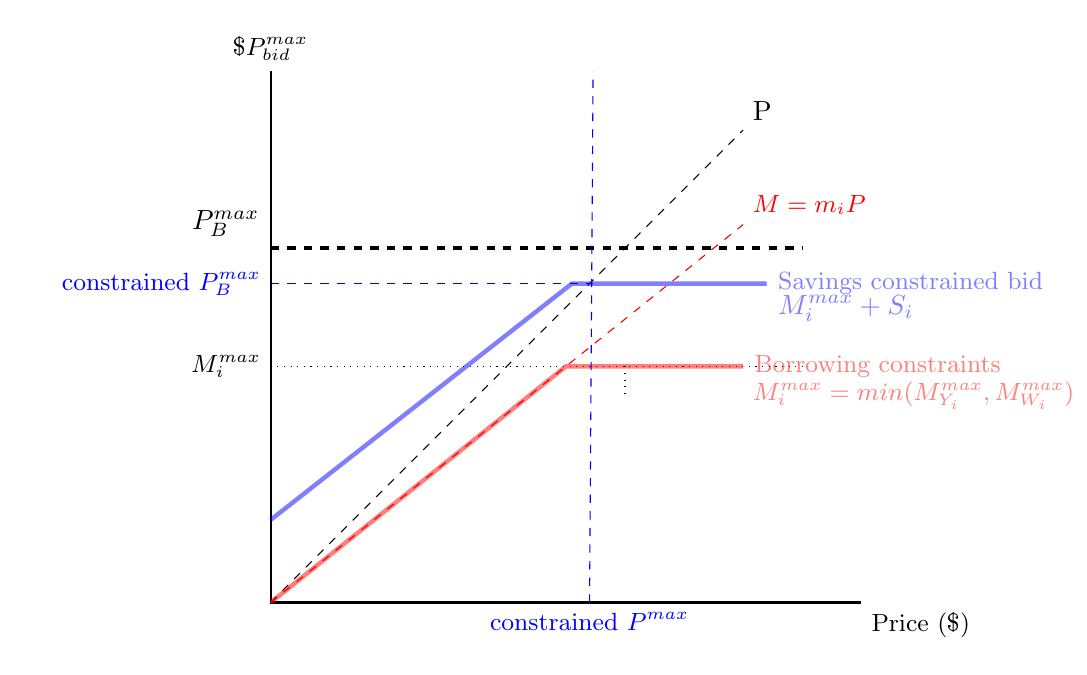
\begin{tikzpicture}	[scale=1.5]
%AXES
\draw[thick] (0,4.5)node[above]{\small \$$P^{max}_{bid}$ } --(0,0)--(5,0)node[below right]{\small Price (\$)};
%\node at (-.25, 3.5)[ rotate=90]{\small Mortgage, Price (\$)};
% M =Mi MAX
\draw[dashed] (0,0)--(4,4)node[above right]{P}; %{\small $P$};
\draw[dotted] (0,2)node[left]{\small $M_i^{max}$}--(4.5,2);%node[right, red]{\small $M = M_i^{max}$};
% M =mi MAX
%\draw[dotted,red, opacity=.5] (0,0)--(4,3.6)node[right]{\small $M = 0.9P$};
\draw[dashed, red] (0,0)--(4,3.2)node[above right]{\small $M = m_iP$};
% COMBINED MAX RED
\draw[ultra thick, red, opacity=.5] (0,0)--(2.5,2)--(4.0,2)node[right]{\small Borrowing constraints};
\node at (4.0,1.95)[below right, red, opacity=.5]{\small $M_i^{max}=min(M_{Y_i}^{max},M_{W_i}^{max})$ };

\draw[ultra thick, blue, opacity=.5] (0,.7)--(2.55,2.7)--(4.2,2.7)node[right, ]{\small Savings constrained bid}node[below right, ]{$M_i^{max}+S_i$};
% SAVINGS
%\draw[-latex] (4,2.05)node[below=5, right] {\small $Savings_i$}--(4,2.69);
% PMAX
% \draw[dashed, ] (3,0)node[below right] {$P_B^{max}$}--(3,4.5);%node[, right]{\small desired max bid};
 \draw[dashed,ultra thick] (0,3)node[above left] {$P_B^{max}$}--(4.5,3);%node[, right]{\small desired max bid};

\draw[dashed, blue, thin] (2.7,0)node[below] {\small constrained  $P^{max}$}--(2.73,4.5); %node[left, text width= 2cm]; %{\small };
\draw[blue, thin, dashed] (0,2.7)node[left] {\small constrained $P_B^{max}$ } --(2.73,2.7);
%node[left, text width= 2cm]{\small savings constrained bid};
\draw[dotted ] (3,2)--(3,1.72);
\end{tikzpicture}
    \caption{Desired bid  and savings + mortgage constrained bid}
    \label{fig:savings-constraint}
    % I removed a line saying Savings sub i in lower corner
    \end{figure}

%
%If you are on the sloped line, constrained by $m$, the price is

% my version
% \begin{equation}
%     P_{B} \le min\Big(  min(m_i P_{B,i}^{max},\ M^{max}_i)+ S_i,\  P_{B,i}^{max}\Big)
% \end{equation}


% HOW DO WE COMPUTE DELTA? 
% \begin{lstlisting}
%     def get_discount_factor(self):
%         """
        
%         The discount factor gives the present value of one dollar received at particular point in the future, given the date of receipt and the discount rate.
%         Delta is the subjective individual discount rate for agent
%         after one year. This will be close to the prime interest rate, r_i.
%         """  
%         self.r_discount= .07
%         delta = 1/ self.r_discount
%         delta_period_1 = 1 / (1 + r_discount) 
%         delta_mortgage_period = delta_period_1**self.mortgage_period
%         #sum_delta = (1 - delta_mortgage_period)/delta
%         #return sum_delta
%         # sum_delta = delta_mortgage_period * (1 - delta_mortgage_period)
% \end{lstlisting}

\subsection{The bargaining model} \label{sec:bargaining-model}
Buyers place bids and a sale occurs if there is a surplus created by the transaction, that is if the the buyer's maximum bid exceeds owner's \gls{reservation price}, the maximum the owner would pay to retain their own property. 
Bargaining models attempt to identify the way the surplus available from a transaction is divided between the parties involved. Possible divisions are described by the red line in Figure~\ref{fig:Nash-bargaining-game}.\footnote{The classic  formulation by John Nash %\cite{Nash_John% (1953-01-01). "Two-Person Cooperative Games". Econometrica. 21 (1): 128–140. doi:10.2307/1906951. JSTOR 1906951, The Nash equilibrium: A perspective. Charles A. Holt and Alvin E. RothAuthors Info & Affiliations March 15, 2004 101 (12) 3999-4002 https://doi.org/10.1073/pnas.0308738101} 
identifies  `\gls{disagreement point},' which which is the  lowest value each player will accept. The combination of reservation price and maximum bid together are the disagreement point for a two-person price bargaining game. Since paying for the house is a negative for the buyer, the scale on the vertical axis  in Figure~\ref{fig:Nash-bargaining-game} is reversed to generate a version of the most common Nash bargaining figure.} 

    \begin{figure}
        \centering
        
  \begin{tikzpicture}[scale=1.5]
%  \draw [gray, opacity=.7] (0,0) grid (7,7);
\draw [<->] (0,6) node[above]{$buyer$}-- (0,0)node[left]{0}node[below]{0} -- (6,0) node[below]{$Seller$};
\draw [red, thick ] (1,7)--(7,1);
\draw [red, line width=1mm] (3,5)--(5,3);
\draw [red, thick, fill= yellow, opacity=.5] (3,3)--(3,5) -- (5,3)--cycle;

% vertical
\draw [blue, dashed] (0,5)node[left]{50,000}--(5,5)node[below right]{will not pay more}--(5,0)node[below]{50,000};
\draw [blue, ] (0,3)node[left]{30,000}--(6,3)node[above right]{can not get more};
% Horizontal
%\draw [blue, dashed] (4,0)--(4,6)node[above right]{will not accept less};
\draw [blue, ] (3,0)node[below]{30,000}--(3,6)node[above right]{can not offer less};
%\draw [ ultra thick] (0,0)--(1.5,1.5)node[ right]{equal set};
%\draw [dashed] (1,1) --(2,1)-- (2,0);
%\draw [red, ultra thick, dashed] (0,0) --(2.4,1.2)node[above]{relative equal set};
%\node at (2,1)[below right, ]{$(max\ u_1,\ max\ u_2)$};
%\node at (3.5,3){Agreement set};\node at (3,3.5){\Large A};

\node at (3,3)[below left, text width=2.8cm, align=right]{\textbf{disagreement\newline point}};
\node[mark size=4pt,color=red] at (3,3) {\pgfuseplotmark{square*}};

\end {tikzpicture}


        \caption{The Nash bargaining game}
        \label{fig:Nash-bargaining-game}
    \end{figure}


In Figure~\ref{fig:Nash-bargaining-game} we imagine the seller values the property at \$30,000 (the reservation price) and the buyer values it at \$50,000 (the maximum bid price).  At any price above \$30,000 the seller is better off. At any price below \$50,000 (above -\$50,000 on the vertical axis) the buyer is better off. 
The set of acceptable bargains acceptable to both is above and to the right of the point labeled `disagreement point.' 

In principle the buyer could pay more than \$50,000 or the seller could accept a price below \$30,000, but neither would do so if they are rational. 
The thick red line segment, called the bargaining set, represents all the outcomes that are\begin{enumerate}
    \item Efficient, because the entire \$20,000 surplus is allocated to the players. 
    \item Feasible, because the players involved gain no more in total than the potential increase in value generated by the transaction.
    \item Rational because neither player has to accept an outcome that makes them worse off.
\end{enumerate}   

The bargaining processes will ideally lead to a point on that thick red line segment. In practice, some of the surplus is dissipated in the sale process, and some is absorbed by intermediaries. We ignore this refinement for the current version of the model. Differences in relative power will tip the outcome in favour of the stronger player.   Players who can afford to wait will get a larger share of the gain. Excess demand favours sellers. Low vacancy rates favour owners over tenants.   If there is a deal, it will still be at a price between the maximum bid and the reservation price, and in most cases probably somewhere near the midpoint. Sellers might reduce the asking price if the home fails to sell in the first period it is on the market.\footnote{Uncertainty adds further complications. Parties may not know each other's disagreement point. PartieS post asking prices greater than their reservation price or initial offers much lower than their true valuation.  
Negotiations often proceed through a series of offers and counteroffers.}\;\footnote{In an overheated housing market bid prices might exceed asking prices, but the price won't exceed the maximum expected profitable bid price, $P_B^{max*}$. We could elaborate the model by defining a measure of \gls{sellers' bargaining power} based on vacancies and expected prices.}   % Ariel Rubinstein \cite{rubinsteinPerfectEquilibriumBargaining1982} presented a convincing solution to the alternating offers model in a 1982 paper. His process converges to the Nash solution. 
% }
%  The higher asking price and lower bids are `cheap talk' (In game theory, cheap talk is communication between players that does not directly affect the payoffs of the game. % This is in contrast to signaling in which sending certain messages may be =


 


% \subsubsection{Maximum bids}
% The rate of return calculation in  Equation~\ref{eqn-property-investment-return1} combined with the investment criterion in Equation~\ref{eqn-property-investment-return2} identifies the maximum  that price that an investor can price offer for a property  and still maker sa profit.

% \begin{align}
% %r^{target}& \le \frac{\delta^\mathbb{T}}{1-m} \left(\dot P_\mathbb{T} - (1+r)^\mathbb{T})m  + \frac{\mathcal{R}_{N, \mathbb{T}}}{P_B^{max}}\right)\nonumber\\
% % (1-m)r^{target}/\delta^\mathbb{T} &\le \dot P_\mathbb{T} - (1+r)^\mathbb{T}m  +   \frac{\mathcal{R}_{N, \mathbb{T}}}{P_B^{max}} \\
% % (1-m)r^{target}/\delta^\mathbb{T} - \dot P_\mathbb{T} + (1+r)^\mathbb{T}m &\le  \frac{\mathcal{R}_{N, \mathbb{T}}}{P_B^{max}}\nonumber\\
% P_B^{max} &\le  \frac{\mathcal{R}_{N, \mathbb{T}}}{(1-m)r^{target}/\delta^\mathbb{T} - \dot P_\mathbb{T} + (1+r)^\mathbb{T}m} \label{eqn:maximum-bid}
% \end{align}

% We call this  $i's$ maximum bid.
% .\footnote{The denominator in Equation~\ref{eqn:maximum-bid} can be seen as an adjusted rate of return for capitalizing net rents, analogous to the value of $r$ in  the standard capitalization formula.} 
% It represents the value of the stream of rent plus any capital gains, and is therefore the most reasonable reservation price for sellers as well the most reasonable maximum offer for potential buyers. In principle it exists for all potential buyers and sellers for every property. In practice, only a subset of potential buyers and sellers are in the market at any time. 


\subsubsection{The many-to-one matching problem}
{The housing market is usually a many-to-many matching problem}: which property goes to which buyer? For each property that comes on the market, there will be a set of potential buyers with differing maximum bids. Some simplifications are available. In each sale, the bidder with the highest bid price among those currently bidding on that property will make the purchase.\footnote{For many reasons the process is likely to exhibit a good deal of randomness and inefficiency. For our purpose, the general messiness of the market is unlikely to do more than slow and blur results somewhat.} Since the highest bidder is competing with the second-highest bidder, we expect the final price to be equal to the second-highest maximum bid, shown as the star in figure~\ref{fig:auction-game}. 


    \begin{figure}
        \centering
        
\begin{tikzpicture}[scale=1]
%  \draw [gray, opacity=.7] (0,0) grid (7,7);
\draw [<->] (0,8.25) node[left, text width=1cm]{Buyer pays}-- (0,0)node[left]{0}node[below]{0} -- (8.25,0) node[below right, text width=1cm]{Seller gets};
\draw [red, thick, latex-latex ](1.5,5.5)node[below left, black, text width=1cm]{Feasible\\ set}-- (2,6)--(6.5,1.5)--(6,1);
\draw [red, line width=1mm] (3,5)--(5,3);
\draw [red, thick, fill= yellow, opacity=.5] (3,3)--(3,5) -- (5,3)--cycle;

% % vertical axis
\draw [dashed] (0,5) node[left] {-\$30,000} -- (3,5) ;
\draw [dashed] (0,3) node[left] {-\$50,000} -- (5.5,3) ;
\draw [dashed] (3,0) node[below]{ \$30,000} -- (3,5.5) ;
\draw [dashed] (5,0) node[below]{ \$50,000} -- (5,3) ;
\draw [dashed, thick, blue] (0,2) node[left] {-\$60,000} -- (7,2)
node [right,text width=2cm]{highest bid};

%  \draw[pattern=north west lines, distance=2mm,pattern color=red!30, draw=none] (0,0) rectangle (3,8);
%  \node[text width=2.5cm] at (1.5,7) {\small Seller will not accept less than \$30,000};

% \draw[pattern=north east lines, pattern color=green!60, draw=none] (0,0) rectangle (9,3);
% \node[text width=2.5cm]at (7,1.5)  {\small Buyer will not pay more than \$50,000};

\draw [ latex-latex, ultra thick](3.7,7)-- (3,7)--(3,3)--(7,3)node[right,text width=2cm]{second highest bid}--(7,3.7)node[above ]{Rational Set} ;
\draw [ latex-, thick, red](3.5,4.5)-- (4,5)--(5.5,5)node[right]{Bargaining Set} ;

\draw [ latex-, thick, red](2.5,5.5)-- (3.6,6.5)--(5.5,6.5)node[right]{Efficient Set} ;%name

%\draw [ latex-, thick, red](3.5,4.5)-- (4,5)--(5.5,5)node[right]{Bargaining Set} ;

%\draw [dashed] (1,1) --(2,1)-- (2,0);
%\draw [red, ultra thick,3 dashed] (0,0) --(2.4,1.2)node[above]{relative equal set};
%\node at (2,1)[below right, ]{$(max\ u_1,\ max\ u_2)$};
%\node at (3.5,3){Agreement set};\node at (3,3.5){\Large A};

\node at (3,3)[left, text width=1.8cm, align=right]{\textbf{\tiny Disagreement\newline point}};

\node[mark size=4pt,color=red] at (3,3) 
{\pgfuseplotmark{square*}};

\node[mark size=8pt,color=blue] at (5,3) 
{\pgfuseplotmark{10-pointed star}};

\draw;
\end {tikzpicture}
        \caption{Auction with a second, higher bid}
        \label{fig:auction-game}
    \end{figure}

%.\footnote{We could allow potential buyers  to approach potential sellers who have not listed with an offer and allow worker-owners to consider retiring early or becoming tenants if an offer is attractive.  This is only likely if speculative pressures are strong. It may require having multiple institutional buyers to make offers more competitive. In that case, initial offers will be closer to the maximum bid price, tending to pull prices up and benefit potential sellers.}  
When there is one bidder, we will employ a simple rule for splitting the gain from trade. Both simplifications are grounded in standard bargaining theory.

 
    \begin{figure}[!thb]
    \centering
    \begin{tikzpicture}
%\draw[step=0.5cm,color=gray] (0,-3) grid (8,7);
\node [above](Bank)at (1,7) {Bank};
\node [above](Buyers)at (5,7) {Buyers $i$};
\node [above](Seller)at (7,7) {Seller};

\draw[ultra thick, -latex](Bank)--++(0,-1.5)node[below]{$P_B^{max}$};
\draw[ultra thick, -latex](Buyers)--++(0,-1.5)node[below]{$P_i^{max}$};
\draw[ultra thick, blue!60,-latex](Seller)--++(0,-1.5)node[below]{$P_R$};

\node[above, red, text width=1.55cm, align=center]at (3,5){Select two highest bids};

\begin{scope}[shift={(0,-1)}]
\draw[ultra thick](1,6.)--(5,6.0); % Bar
\draw[ultra thick, blue!60,-latex](7,6.2)--++(0,-1)--++(-4,0)node[left, red]{Compare};  %Pass P_R to if-then
\draw[ultra thick, -latex](3,6)--++(0,-1.5)--++(-2.,-.5);% down and left
\draw[ultra thick, -latex](3,5)--++(0,-1)node[below, text width=1.5cm, align=center]{None above {$P_R$} };%
\draw[ultra thick, -latex](3,5)--++(0,-.5)--++(2.2,-.5)node[below, text width=1.cm, align=center]{One above {$P_R$} };
% down and Right

\draw[ultra thick, -latex](.1,2.5)node[above, text width=2.cm, align=center]{Two or more above {$P_R$} }--++(0,-.75)node[below, text width=3cm, align=center]{Auction: price is second highest $P_i^{max}$, house goes to highest bidder};

\draw[ultra thick, -latex](3,2.5)--++(0,-.75)node[below, text width=2cm, align=center]{No sale};

\draw[ultra thick, -latex](5.5,2.5)--++(0,-.75)node[below, text width=2cm, align=center]{Bargain: price is power-modified mean};
\end{scope}

\end{tikzpicture}
    \caption{The bargaining model and price determination}
    \label{fig:Bargaining}
    \end{figure}



\subsubsection{The bargaining process}
We have now identified a set of bids and a reservation price for each property on the market that must be converted to a price for that property using the bargaining rule. 
The bargaining  mechanism then simply has to compare the maximum bid price $P_B$ with the seller's reservation price. If the $P_B^{max}>P_R$, a deal that is between the two values is possible. Otherwise, the transaction does not proceed.
If a bargain is possible, the rule is simple: 
\begin{enumerate}
    \item If there is only one maximum bid above the reservation price, split the difference between the bid and the reservation price evenly.\footnote{It is fairly simple if perhaps not very revealing to incorporate relative power. % as described in Footnote~\ref{fn:relative-power}.
    }
    If $P_B^{max}>P_R$,  the bargaining rule selects a value 
    \[P = xP_B^{max}+(1-x)P_R, \ \ \ x\in [0\dots 1] \]
where $x$ is typically 0.5.
    \item If there are two or more maximum bids above the reservation price, the property goes to the highest and since the bids are the maximum the buyers would pay under any circumstances, the price is set a the second highest bid in order to reflect the tightness of the market.\footnote{This is an application of Vickrey \gls{second-price auction} theory\cite{levinAuctionTheory2004}.} 

\end{enumerate}
 
% \[P^{ask}>P_M^e> 0.95 P^r\]
% Otherwise
% \[P^{ask}> 1.10P^r>P_M^e\]
% If no offer exceeds the reservation price, no sale is made.

% Once an owner reached retirement age, if no sale is made the reservation price is reduced for the next cycle.
% If no sale is made the owner considers becoming a landlord. if the present value of net rent is above the reservation price, the owner rents out the home. 


\section{Linking financialization and urban productivity}
% {\color{red}We model a relationship between productivity and agglomeration. }
As we point out in Chapter~\ref{chapter-tramsmission} there are numerous channels through which financialization might affect the productivity of the city. The available literature does not tell us which channels are active,  and which, if any, have a significant effect. Our goal in modelling is to establish whether or not linkages are likely to have significant effects on the economy. If our model establishes that the effects are potentially significant, it might encourage researchers to explore this neglected area in urban economics.

To introduce the potential effect of financialization and ownership as simply as possible, we rewrite $A$ from the basic model ``as:\[ A= A_0 + effectiveness*share * rent*\]
where $A_0$ represents outside or general factors contributing to productivity, $0<effectiveness<1$ is how much the local share of rents matters, and  $share*rent$ stands for the share of the urban locational rents captured by residents and contributing to local productivity. That there are local factors is indicated by the variability of estimates of $A$ in empirical studies.\footnote{See Chapter~\ref{chapter-tramsmission} Subsection~\ref{sec-fig-residuals} for references and an illustration.} 
The share term is itself a composite of the actual land-ownership share of residents determined by the housing market and the propensity to invest locally.

In the class of models we draw on, the scale parameter $A$ controls the overall productivity. It might capture a range productivity-enhancing effects: the contribution of urban infrastructure (including transportation infrastructure), technology, ownership ratios, participation by residents, local investment in productive capital, regulatory structure, the presence of local universities, the skill level of the supporting workforce, the complexity of supply chains, or other factors. None of these are explicit inputs in our model in the way technology is in some of the growth literature described in Chapter~\ref{chapter-growth}.\footnote{Public inputs like the transportation system do not appear directly any of the models.} 
Missing explanatory variables are likely to inflate the residuals in estimates of $A$.
% The channels we discussed in  Chapter~\ref{chapter-tramsmission}  all have their influence on the \gls{Alonzo-Jacobs cycle} in our model, either through a reduction in the inputs to production, labour and capital, or by changing parameters  $A$, $\alpha$, $\beta$, or $\gamma$ of the production function. 
It is likely to be difficult to disentangle influences on the parameters empirically, this simple model makes it possible to study the effect of a range of linkages without. % Their effects on productivity are all positive. They are each likely to have several components, including common components, and measurement at the level of a city would involve aggregating many firms in many industries.     

 
\section{Summary}
In this chapter we developed the rules that agents in our agent-based model follow. In doing this we have defined variables and institutional features, and developed a description of the bargaining process behind all of the adjustments. The formulae developed here are implemented in the python simulation model. % In the second part of this chapter, we documented the agent based modeling code using the ODD standard.  
Appendix~\ref{appendix-parameters} contains the parameter values used for the model.  % Details of the adjustment speeds and parameter setting are not discussed here because they have to be `tuned'. The parameter space of the model is large, and cities only exist in a sub-region of the space. For example, if the marginal product of labour is too low, cities cannot exist. If it is too high the city explodes. We have identified a region with plausible values in which city behaviour corresponds to what we know about the evolution of cities. 

 We use equilibrium conditions for competitive labour markets to bypass the complex and partially understood wage-setting process. We apply a standard theoretical result from the theory of the firm, that workers are paid their \gls{marginal value-product}. We ground our approach in recent research that has derived and estimated an aggregate urban production function consistent with modern \gls{neoclassical growth theory}.\footnote{We are not aware of other research that has taken this step yet.} Our augmented representative firm determines the urban wage premium that drives city growth. We assume that, since housing and labour markets can adjust more quickly than urban productivity, the production sector responds continuously to the slower movement of population and productivity. % need to reference? 
%We employ \gls{equilibrium reasoning} in the housing and investment process. '
We also assume investors behave rationally in that they estimate the potential returns on their investments and seek the highest returns they can get. They calculate an offer price in each transaction based on several factors: land rents, expected price changes, their price of capital and discounting rate, and other information available to them. We do not, however, impose an equilibrium on the housing market.

The relationships set out in this chapter are theoretically grounded and realistic. They allow us to implement the three sub-models described in the introduction to this thesis in code. The resulting simulation model lets us demonstrate some implications of standard urban economic theory that were plausible a-priori, but that have not been formally demonstrated before.  



\end{document}